\chapter{Stimuli Selection}
\label{ch:3}

\section{Introduction}

The current study aims to investigate native (L1) English speakers’ accentedness judgment on non-native (L2) English speech samples. To this end, 100 L2 audio speech samples served as stimuli for two perception studies. These two studies are discussed in Chapters 4 and 5. This chapter describes how the stimuli were selected. 

The 100 L2 speech samples were selected from the Speech Accent Archive (SAA: \citealp{Weinberger_saa_2019}). Audio samples in the SAA are phonetically transcribed by trained phoneticians using the International Phonetic Alphabet (i.e., IPA). These transcriptions reflect the transcribers’ perception. The 100 L2 speech samples were selected primarily based on their respective IPA transcriptions. Although care has been taken by the SAA personnel in providing relatively reliable transcriptions, inaccuracies could still exist. Therefore, the current study conducted acoustic analysis on the samples to further evaluate the reliability of the IPA transcriptions. 

In addition to the 100 L2 speech samples, speech samples from 50 L1 speakers of American English were also extracted from the SAA to evaluate the acoustic difference between L1 and L2 speech samples. Mean acoustic measurements of these 50 L1 speech samples were used as an approximation for native speaker norms. If the acoustic difference between an L2 speech segment and its native speaker norm could be captured by the IPA transcription for the L2 speech segment, then the IPA transcription is considered reliable and is used in the current study. 

Some of the acoustic measurements described in this chapter were further utilized in Experiment 2 (Chapter 5) to see how they correlate with perceived accentedness.  It should be noted that acoustic correlates of a phoneme are numerous and could vary depending on adjacent phonological contexts and sometimes extra-linguistic factors such as age \citep{Holt_2010}. Consequently, a few acoustic measurements cannot fully capture all of the features of a phoneme. To avoid the complexity of acoustics-to-phoneme mapping, the current study selected the stimuli primarily based on the IPA transcriptions, which are reflective of perception. The acoustic analysis described in this chapter serves mainly to verify the IPA transcriptions. The following section describes how stimuli selection and acoustic verification were carried out. 

\section{Corpus}

The 100 L2 stimuli are short two-word speech samples selected from the SAA. The SAA, as of June 2019, consists of 2786 audio speech samples produced by both L1 and L2 English speakers. All samples consist of speakers reading the sample paragraph given below:

\bigskip
\noindent \textbf{The ``Stella" Passage:}

\noindent \textit{Please call Stella. Ask her to bring these things with her from the store. Six spoons of fresh snow peas, five thick slabs of blue cheese, and maybe a snack for her brother Bob. We also need a small plastic snake, and a big toy frog for the kids. She can scoop these things into three red bags, and we will go meet her Wednesday at the train station.}
\bigskip

The speakers also provided their demographic information (e.g., age, gender, native language, age of English onset, learning style, current and former residence, etc.), which is publicly available on the SAA website. The speech samples were all digitally recorded by trained experimenters in the acoustic lab at George Mason University or somewhere else where the speakers and the experimenters deemed suitable. Only CD-quality (16-bit/44kHz) recordings are included in the archive. Low quality recordings are not accepted \citep{Weinberger_2011}.

The audio samples were narrowly transcribed using the IPA by at least three transcribers. The transcribers were phonetically trained graduate students at George Mason University. The IPA transcriptions were reached by the consensus of at least three people. All transcriptions were vetted and made available online by the administrator (i.e., Dr. Steven Weinberger) of the SAA. 

It should be mentioned that speech samples in the SAA were not transcribed by the same group of transcribers. Although most of the transcribers are L1 speakers of American English, some of them are international students whose native language is not English. Dr. Weinberger administered quality control by training all the transcribers through a semester-long, graduate-level phonetics class. Transcribers were instructed to follow the same guideline when transcribing the speech samples. To improve accuracy and resolve disagreements among the transcribers, speech processing software such as PRAAT \citep{Boersma_2015} or Audacity \citep{Mazzoni_2000} were often used to analyze benchmark acoustic signals. Around 1300 speech samples have been transcribed and are available online. An example is given below:

\bigskip
\noindent [pʰli:z kɔ:l stɛla ɛsk ɜ˞ tu bɹɪ̃ŋ ðɪ θɪ̃ŋs wɪθ hɜɹ fɹɔ̃m θə stɔ:ɹ sɪks ɪ̆spũ:nz ɔf fɹɛʃ snoʊ pʰi:z faɪf θɪk slɛ:bz̥ ɔv blu: tʃi:z ɛ̃n meɪbi ə snɛ̃:k fɔɹ hɛɹ bɹʌðəɹ bɑ:b̚ wi ɔlso nid̥ ə smɔ:l plɛ̞:stɪk sneɪk ɛ̃n ə bik t̪ɔɪ fɹɑ:ɡ fɔr ðə kɪ:ts ʃi kɛ̃n sku:p̺ ði:z θĩnks ɪ̃ntu θɹɪ ɹɪd bɛɡz ɛ̃n wi wɪl ɡoʊ mi:t hɛɹ wẽnɪzdeɪ æ d̪ə tɹeĩn steɪʃə̃n] (SAA: arabic23)
\bigskip

The vetted IPA transcriptions in the SAA were previously utilized by researchers in computational linguistics (e.g., \citealp{Frost_2013, Minematsu_2014}) and second language acquisition (e.g., \citealp{Klein_2011}). Recently, \citet{Weinberger_2019} recruited an additional 67 phonetically trained transcribers to transcribe a selection of audio clips from the archive. The results show that 72\% of the 67 participants’ transcriptions matched the vetted ones, lending support to the reliability of the vetted transcriptions. 

\section{Types of Stimuli}

The 100 L2 speech samples for the current study were selected based on the vetted transcriptions available in the SAA. These samples were further grouped into four types based how they differ from their L1 target productions. This section describes the determination of L1 target productions, and the four types of stimuli used by the current study.

\subsection{L1 Target Productions}

The L1 target productions were defined as the most common L1 productions. Such a treatment was based on the assumption that L1 American English listeners would all be familiar with the most common L1 productions and consequently rate them as native-like. To find the most common L1 productions, the current study surveyed productions from 100 L1 speakers of American English in the SAA (See Appendix A for demographic information). The most common productions among these speakers were considered L1 target productions. For example, 90\% of the L1 productions for the word ``\textit{thick}" are [θɪk]. [θɪk] was therefore chosen as the L1 target production for “\textit{thick}.” IPA transcriptions of these L1 American English speakers were also used to build a computational model to approximate English phonetic and phonological grammar. Chapter 6 discusses the model in detail.

For the two perception experiments, the current study selected 100 L2 speech samples as stimuli. L2 speech samples that were transcribed the same as their L1 target production (e.g., [θɪk] for ``\textit{thick}") were termed the “match” stimuli, meaning that the L2 productions match their L1 target productions. L2 productions that do not match their L1 target productions were termed the “mismatch” stimuli.  Some of the mismatch stimuli are not unique to L2 speakers of English. For example, some L1 speakers pronounce ``\textit{thick}" as [tɪk] according to data on the SAA. Since [tɪk] does not match the L1 target [θɪk],  [tɪk] was nevertheless termed as a mismatch stimulus. Presumably, the mismatch stimuli that are observed in L1 speech data would be judged as less accented. The “mismatch” that are not observed in L1 speech data (e.g., pronouncing “\textit{ask}” as [æskə]) would be judged as more accented. 


\subsection{Four Types of Stimuli}

The mismatch stimuli were further divided into three groups based on three types of mismatches, namely, stimuli with consonant mismatches (e.g., [tɪk] for “\textit{thick}”), stimuli with vowel mismatches (e.g., [θik] for “\textit{thick}”), and stimuli with syllable structure mismatches (e.g., [faɪvə] for “\textit{five}”). Therefore, the 100 stimuli were divided into four types (i.e., the match type and the three types of mismatches). 

Table \ref{table:tos} illustrates the four types of stimuli. IPA transcriptions in the match stimuli column represent the most common L1 pronunciations for the five phonological contexts. 25 of the 100 L2 stimuli were transcribed the same as the IPA transcriptions listed in the match column. These 25 L2 speech samples were called the match stimuli \footnote{[æsk (h)əɹ] in the match column means that both [æsk əɹ] and [æsk həɹ] are equally common in the SAA.}. The remaining 75 are mismatch stimuli. They differ from the match stimuli by only one phonetic element. For example, stimulus [faɪv tɪk] differs from its corresponding match stimulus [faɪv θɪk] by only one consonant (i.e., [θ]$\rightarrow$[t]). Stimulus [faɪv tɪk] therefore contains only one consonant mismatch. Among the 75 mismatch stimuli, 25 contain only one consonant mismatch (five stimuli for each context), 25 contain only one vowel mismatch (five stimuli for each context), and 25 contain only one syllable structure mismatch (five stimuli for each context). 

\begin{table}[!h]
  \figSpace
  \centering
  \caption{Types of Stimuli}
\label{table:tos}
    \begin{tabular}{p{5.2em}llll}
    \toprule
    Context & \multicolumn{1}{p{5.2em}}{Match} & \multicolumn{1}{p{5em}}{Consonant\quad Mismatch} & \multicolumn{1}{p{5em}}{Vowel\quad Mismatch} & \multicolumn{1}{p{5em}}{Syllable Mismatch} \\
    \midrule
    \textit{please call} &[pʰliz kʰɑl] &[\textbf{p}liz kʰɑl]&[pʰliz kʰ\textbf{o}l]&[pʰ\textbf{ə}liz kʰɑlˠ]\\
        \textit{ask her} &[æsk (h)əɹ] &[æsk hə\textbf{r}]&[\textbf{ɑ}sk həɹ]&[æs\underline{ } həɹ]\\
        \textit{six spoons} &[sɪks spunz] &[sɪks spun\textbf{ʃ}]&[s\textbf{i}ks spunz]&[sɪks \textbf{ə}spunz]\\
        \textit{five thick} &[faɪv θɪk]&[faɪv \textbf{t}ɪk] &[f\textbf{a}v θɪk]&[faɪv\textbf{ə} θɪk]\\
        \textit{small plastic} &[smɑl pʰlæstɪk]&[smɑ\textbf{ɭ} pʰlæstɪk]&[smɑl pʰlæst\textbf{i}k]&[smɑl pʰlæs\underline{ }ɪk] \\
    \bottomrule
    \end{tabular}%
    \figSpace
\end{table}%

\section{Acoustic Comparisons}

The 100 L2 stimuli represented 11 types of consonant mismatches, five types of vowel mismatches and two types of syllable structure mismatches. The stimuli were chosen mainly based on the IPA transcriptions available in the SAA. In order to verify the IPA transcriptions, acoustic analyses were carried out to compare benchmark measurements between the L1 and L2 speech samples. The aim of the following acoustic analysis is to verify whether acoustic differences between an L2 stimulus and its corresponding L1 speech samples can be captured by the IPA transcription of the L2 stimulus. For example, if an L2 segment was transcribed as an aspirated [pʰ], while its corresponding L1 productions are the non-aspirated [p]s. The [ʰ] symbols suggests that the L2 segment has a longer voice onset time (VOT) than the L1 [p]s. To verify whether the [pʰ] was correctly transcribed, the current study measures the duration of the L2 VOT and the mean VOT of L1 [p]s. If the L2 VOT is indeed longer than the mean L1 VOT, then the current study accepts [pʰ] as a correct transcription for the L2 segment.  

L1 English speech samples from the SAA were selected for the determination of what might constitute native speaker pronunciation norms. The speech samples were produced by 50 L1 speakers of American English. They were from 21 states in the continental U.S., ages from 18 to 79 (M=39.67, SD=16.62). 25 of them are male, the other 25 are female. Detailed demographic information of these 50 L1 speakers is listed in Appendix A.  

A large body of previous research has demonstrated that phonemic categories are distinguished
by multiple acoustic cues (e.g., Lisker, 1986; Toscano and McMurray, 2010). For example, VOT, pitch of the following vowel, and other 14 kinds of acoustic cues could be responsible for the distinction between /pa/ and /ba/ (Lisker, 1986). The current study opts to focus on the primary and most robust cues as identified by previous speech perception research, while fully acknowledging that other phonetic cues could also affect speech perception.


\subsection{Segmentation}

All the L1 and L2 speech samples were first segmented. The intensity of the speech samples was normalized to 75dB using PRAAT. Initial phoneme segmentation of the speech samples was performed with the Montreal Forced Aligner \citep{McAuliffe_2017}. This is a newly developed neural network-based aligner that is comparable to human annotators and provides better performance than the traditional Penn Phonetics Lab Forced Aligner \citep{Yuan_2008}. Errors or inaccuracies discovered in the auto-segmentation were manually corrected. Relevant acoustic measurements were extracted via a PRAAT script for further analysis. Figure \ref{fig:seg} illustrates the results of the automated alignment, where the top row displays information of the spectrogram and formants and the second row from the top displays pitch (dotted line) and intensity (solid line) contours. The third row from the top represents phone boundaries using the Arpabet symbols and the bottom row shows word boundaries.

\begin{figure}[ht]
  \figSpace
    \centering
	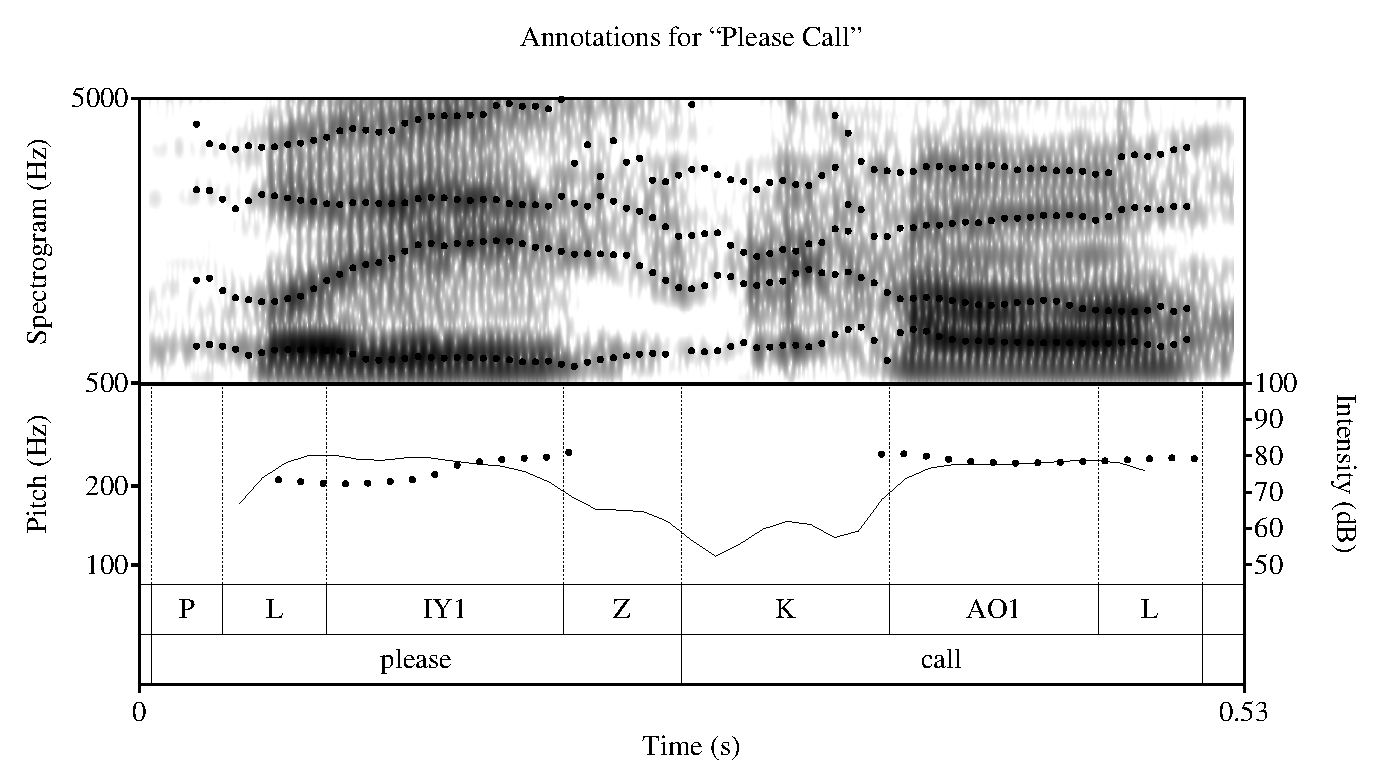
\includegraphics[width=0.8\textwidth]{figures/seg.eps}
    \caption{Illustration of Auto-segmentation}
    \label{fig:seg}
  \figSpace
\end{figure}

\subsection{Plosives}

Six L2 speech samples selected by the current study contained plosive-related mismatches as indicated by their respective IPA transcriptions. The following describes how the mismatches were verified by acoustic measurements. Duration of voice onset time (VOT) was used as the benchmark acoustic measurement for plosives. VOT duration of L2 segments and mean VOT duration of L1 segments were measured. 

VOT is defined as the interval between the onset of a plosive burst and the onset of the following vocalic onset. There are numerous claims that VOT directly affects accentedness perception \citep{Major_1987, Riney_1999}. Six L2 stimuli were therefore selected to verify these claims made in previous research. Following the practice of \citet{Chodroff_2017}, the beginning of the VOT was placed at the beginning of a plosive burst release; and the endpoint was placed at the beginning of periodicity in the waveform or a visible pitch track, whichever came first. VOT labeling was initially achieved in PRAAT with the AutoVOT plugin \citep{Keshet_2014}. Labeling errors were manually corrected in PRAAT based on waveforms and spectrograms. 

Contexts “\textit{please call},” “\textit{small plastic}” and “\textit{six spoons}” were used for the investigation of VOT-related consonant mismatches. Six L2 speech samples that were identified as having VOT-related mismatches were extracted for analysis. Two speech samples involved VOT-shortening on [kʰ] in the word “call,” one speech sample involves VOT-shortening on [pʰ] in the word “please,” one speech sample involves VOT-shortening on [pʰ] in the word “\textit{plastic},” two speech sample involve VOT-lengthening on [p] in the word “\textit{spoons}.” In addition to the L2 speech samples, VOTs of 50 L1 speech samples were measured for comparison. 

Table \ref{table:vot} illustrates the type of VOT-related consonant mismatches and the contexts where they occurred. Every row in Table \ref{table:vot} represents the VOT of a plosive segment. The mismatch column lists the type of VOT-related mismatches and the segments involved. The L2 VOT column contains durational measurements of the six L2 VOTs. L2 VOTs were converted to z-scores with regard to L1 English VOT means and standard deviations (SD). A z-score represents how many standard deviations an L2 VOT mean is from the mean L1 VOTs. A positive z-score means an L2 VOT is longer than the mean L1 VOT, while a negative z-score means an L2 VOT is shorter than the mean L1 VOT.

For example, the first row of Table \ref{table:vot} shows that an L2 stimulus “\textit{please call}” involves the de-aspiration of [kʰ] in the word “call.” The L2 segment [k] has a VOT of 33.01 milliseconds (ms). Calculation based on 50 L1 American English productions of “\textit{please call}” shows that the mean VOT of L1 [kʰ]s is 52.78 ms with a standard deviation of 13.71 ms. The z-score shows that the L2 VOT is 1.44 standard deviations below the L1 mean. 

\begin{table}[!h]
  \figSpace
  \centering
  \caption{L1 and L2 VOT Comparisons}
\label{table:vot}
    \begin{tabular}{llrrr}
    \toprule
   Contexts & Mismatches & L2 VOT (ms) & L1 (English) VOT (ms) & Z \\
    \midrule
    \textit{please call} & [kʰ]$\rightarrow$[k] & 33.01 & M=52.78; SD=13.71 & -1.44 \\
    \textit{please call} & [kʰ]$\rightarrow$[k] & 21.26 & M=52.78; SD=13.71 & -2.30 \\
    \textit{please call} & [pʰ]$\rightarrow$[p] & 10.05 & M=62.50; SD=18.06 & -2.91 \\
    \textit{small plastic} & [pʰ]$\rightarrow$[p] & 20.86 & M=62.84; SD=15.53 & -2.70 \\
    \textit{six spoons} & [p]$\rightarrow$[pʰ] & 45.33 & M=14.46; SD=7.15 & +4.32 \\
    \textit{six spoons} & [p]$\rightarrow$[pʰ] & 68.53 & M=14.46; SD=7.15 & +7.56 \\
    \bottomrule
    \end{tabular}%
  \figSpace
\end{table}%


As shown in Table 3.2, the shortened VOTs are indeed shorter than the L1 means, while the lengthened VOTs are indeed longer than the L1 means. Therefore, VOT differences between the L1 and L2 speech samples were successfully captured by the IPA transcriptions of the L2 speech sam- ples. These L2 speech samples were therefore chosen to represent VOT-related phonetic mismatches in L2 speech.

\subsection{Fricatives} 

Seven L2 stimuli were selected to investigate the perceptual accentedness of fricative-related mismatches. Four stimuli involve replacing L1 fricatives with other fricatives (e.g., [z]$\rightarrow$[s], [θ]$\rightarrow$[f]). Three stimuli involve replacing the interdental fricative /θ/ with /t/. The seven stimuli are listed in Table \ref{table:cog}. Analysis in this session concerns three types of benchmark acoustic signals, namely, Center of Gravity, pitch context, and noise ratio. These acoustic signals were selected to approximate differences in place and manner of articulation.

\subsubsection{Center of Gravity}

Previous research on the acoustic correlates of English fricatives has discovered that the Center of Gravity (COG) of fricatives is a reliable cue for place of articulation \citep{Jongman_2000}. COG is a measurement of energy concentration. Energy of a speech sound, as measured by amplitude, could be concentrated in either the higher frequencies or the lower frequencies of the sound. A smaller COG implies that the energy of a sound is concentrated in the lower frequencies. 

As a measurement for place of articulation, COG value decreases as place of articulation moves further back in the oral cavity. For example, alveolar fricatives (e.g., /s/ and /z/) have lower COGs than dental fricatives (e.g., /θ/ and /ð/), whose COGs are lower than labiodental fricatives (e.g., /f/ and /v/) (Jongman et al., 2000). Although COG is traditionally thought of as a cue for place of articulation, \citet{Jongman_2000} reported that COG is also a good indicator for voicing, with voiceless English fricatives having significantly higher COGs than their voiced counterparts. Table \ref{table:cog} lists the COGs of segments in the seven L2 and L1 stimuli selected by the current study.

% Table generated by Excel2LaTeX from sheet 'cog'
\begin{table}[h]
  \figSpace
  \centering
  \caption{L1 and L2 COG Comparisons}
\label{table:cog}
    \begin{tabular}{llrlr}
    \toprule
    Contexts & Mismatches & L2 COG (Semitone) & L1 COG (Semitone)&Z \\
    \midrule
    \textit{please call} & [z]$\rightarrow$[s] & 77.68 & M=71.14; SD=5.31 & +1.23 \\
    \textit{small plastic} & [s]$\rightarrow$[z] & 64.39 & M=71.30; SD=7.28 & -0.95 \\
    \textit{five thick} & [θ]$\rightarrow$[f] & 73.77 & M=64.37; SD=11.40 & +0.82 \\
    \textit{six spoons} & [z]$\rightarrow$[ʃ] & 71.10  & M=64.56; SD=8.86 & +0.73 \\
\textit{five thick}& [θ]$\rightarrow$[t̪] & 59.63 & M=64.37; SD=11.40 & -0.42 \\
\textit{five thick}& [θ]$\rightarrow$[t̪] & 63.27 & M=64.37; SD=11.40 & -0.10 \\
  \textit{five thick}& [θ]$\rightarrow$[t̪] & 42.63 & M=64.86; SD=9.71 & -2.29 \\
    \bottomrule
    \end{tabular}%
  \figSpace
\end{table}%

Every row of Table \ref{table:cog} shows the COGs of an L2 segment and the corresponding mean L1 COG value. For example, the first L2 stimulus is “\textit{please call}.” The coda of “\textit{please}” was transcribed as [s]. The L2 production therefore involves the devoicing of the [z] in “\textit{please}” (i.e., [z]$\rightarrow$[s]). The COG of the L2 segment [s] is 77.68 semitones, while its corresponding L1 segment [z] has a mean COG of 71.14 semitones with a standard deviation of 5.31. The L2 segment [s] is thus 1.23 standard deviations above the mean. This result is consistent with previous claims that COGs of voiceless fricatives are higher than COGs of their voiced counterparts. Therefore, the [s] was accepted by the current study as a correct transcription.

The second L2 stimulus “\textit{small plastic}” replaced the [s] in “\textit{small}” with a voiced [z]. The COG of this L2 segment [z] is lower than the mean COG of the corresponding L1 [s]s. This finding is also consistent with previous research, which showed that voiced fricatives have lower COGs than voiceless fricatives \citep{Jongman_2000}. Acoustic measurements for the third stimulus  show that the L2 segment [f] has a higher COG than its L1 target segment /θ/, which is consistent with previous findings that COG value increases as the place of articulation moves further front in the oral cavity \citep{Jongman_2000}. Given these results, the IPA transcriptions for the first three stimuli in Table \ref{table:cog} were considered accurate by the current study. The difference between the remaining four L2 stimuli and their corresponding L1 productions cannot be explained via the COG measurement. The following section discusses two additional acoustic measurements that could capture the difference between the remaining four L2 stimuli and their corresponding L1 productions.  

\subsubsection{Pitch Context}

The fourth L2 stimulus “\textit{six spoons}” changed the final consonant in “\textit{spoons}” from [z] to [ʃ]. The COG of the voiceless L2 segment [ʃ] is higher than the mean COG of its target L1 segment [z]. Previous research claimed that the COG of the post-alveolar fricative [ʃ] should be lower than both alveolar fricatives /s/ and /z/ \citep{Jongman_2000}. Based on the COG measurement, [ʃ] is perhaps not a correct transcription. However, acoustic correlates of English phonemes are multidimensional. COG values alone cannot explain why the final consonant of “\textit{spoons}” was transcribed as [ʃ]. 

In addition to COG values. the perception of /s/ and /ʃ/ could be affected by the pitch values of the preceding segments \citep{Niebuhr_2017}. Specifically, /s/ is more likely to be perceived as /ʃ/ when its preceding segment carries a higher pitch. In other words, the final consonant in “\textit{spoons}” could be an /s/, but was perceived and transcribed as [ʃ] because the penultimate segment /n/ carries a relatively higher pitch. To investigate whether the preceding pitch context of the final consonant in “\textit{spoons}” potentially affected transcribers’ perceptions, pitch values of the /n/s were extracted in PRAAT. Pitch values were extracted at the location of the energy peak in the amplitude spectrum, using methods described in \citet{De_Jong_2009}. Pitch values were converted to semitones relative to 100 Hertz to approximate the non-linear mapping between Hertz values and human perception. 

The L2 stimulus “\textit{six spoons}” was produced by a male Lamaholot speaker. The [n] of the L2 stimulus carries a pitch of 20.98 semitones. To calculate pitch values of the natively produced /n/s, productions of 25 male L1 American English speakers were similarly processed in PRAAT. Results showed L1 male speakers’ productions of the /n/ carry a mean pitch of 14.93 semitones, with the standard deviation of 3.27 semitones. The L2 /n/ thus indeed carries a relatively higher pitch than mean pitch values of the L1 /n/s. Therefore, there is a reason to believe that the pitch value of the penultimate consonant [n] in the L2 production of “\textit{spoons}” affected transcribers’ perception of the final consonant. This finding does not necessarily imply that the IPA transcriptions of the L2 stimulus are incorrect, but affirms the fact that acoustic correlates of phonemes are multidimensional. Therefore, the current study accepted the [ʃ] as a correct transcription.

\subsubsection{Noise Ratio}

In addition to the four stimuli analyzed above, there are three stimuli that involve the replacement of the dental fricative /θ/ with a dentalized [t̪]. As discussed above, COGs increase as the place of articulation moves farther front in the oral cavity. Therefore, dental [θ]s should have higher COGs than [t̪]s. Table \ref{table:cog} shows that the mean L1 COG of [θ]s is indeed higher than COGs of the [t̪]s. However, the difference between /θ/ and /t/ lies primarily on their respective manners of articulation, which is not captured by COG measurements. To inspect whether the [t̪]s are reliable transcriptions, the current study opted to use noise ratio to investigate the manner difference between fricative and plosive consonants.

Plosive consonants, such as the alveolar /t/, consist of a silent closure interval, which is followed by a frication noise burst and an interval of aspiration noise. Fricative consonants, such as /θ/, also consist of a silent closure interval, which is followed by a period of friction noise. The longer the closure interval, the more likely a fricative is perceived as an affricate \citep{Dorman_1980}. The shorter the duration of friction noise, the more likely a fricative is perceived as a plosive \citep{Dorman_1980}. 

To investigate durational measurements of the American English /θ/, the same 50 American English speakers’ productions of “\textit{five thick}” were used. Male and female samples were analyzed separately, because frication noise of females tends to be shorter than males \citep{Jongman_2000}. 

A possible confounding factor of durational measurements is speech rate. Intervals of closure and frication noise might be shortened in fast speech. In slow speech, the intervals could be lengthened. To control for speech rate, noise ratios were calculated. Noise ratios were defined as the ratio of fricative noise duration over the duration of the whole word \citep{Jongman_2000}. Word duration was defined as the interval between the onset of the frication to the end of the word. Closure intervals were not included in the total duration of a word, because the L1 and L2 segments are word initial. It is difficult to distinguish closure intervals of word-initial segments from speech pauses between words. Tabel \ref{table:nr} illustrates the noise ratios of the L1 and L2 segments.

% Table generated by Excel2LaTeX from sheet 'noise'
\begin{table}[!h]
  \figSpace
  \centering
  \caption{L1 and L2 Noise Ratio Comparisons}
\label{table:nr}
    \begin{tabular}{lllrr}
    \toprule
    Phrases & Gender & Mismatches & L2 Noise Ratio & L1 Noise Ratio \\
    \midrule
    \textit{five thick} & male  &  [θ]$\rightarrow$[t̪] & 0.17  & 0.25 \\
   \textit{five thick} & male  & [θ]$\rightarrow$[t̪] & 0.15  & 0.25 \\
   \textit{five thick} & female & [θ]$\rightarrow$[t̪] & 0.16  & 0.20 \\
    \bottomrule
    \end{tabular}%
  \figSpace
\end{table}%

The mean noise ratio for male L1 speakers is 0.25 (SD=0.06), and the mean noise ratio for female L1 speakers is 0.20 (SD=0.08). For the three L2 stimuli that replaced /θ/ with [t] or [t̪], noise durations were defined as the duration of the release burst and the aspiration noise. Word durations were defined as the interval from the onset of the release burst to the end of a word. As shown in Table \ref{table:nr}, the noise ratios for [t̪]s are 0.17, 0.15, and 0.16 respectively. In other words, L1 [θ]s, in general, have a longer frication noise duration than the noise durations (i.e. burst and aspiration noise) of the three corresponding L2 segments. Since shorter noise duration of a segment increases the chance for it to be perceived as a plosive consonant \citep{Jongman_1989}, there is reason to believe that the three L2 segments were transcribed correctly. These L2 stimuli were therefore accepted by the current study as representatives of /θ/-stopping (i.e., /θ/$\rightarrow$/t/). 

\subsection{Liquids}

In addition to plosives and fricatives, the current study also aims to investigate the accentedness of liquid productions in L2 speech. L2 speech involving the alternation between /ɹ/ and /l/ was often perceived by L1 American English listeners as very accented \citep{Riney_2005}. Eight L2 speech samples were selected to investigate the accentedness of syllable final /l/s and /ɹ/s. Based on findings in previous research, the degree of /l/-velarization was approximated by the difference between F1 and F2 \citep{Riney_2005} values. The degree of /ɹ/-rhoticity was approximated by the difference between F2 and the third formant frequencies (F3) \citep{Ohala_2001}. The F1, F2, and F2 values were extracted at the energy peak in the amplitude spectrum of the liquids.The following section discusses the analysis on L1 and L2 liquid productions in the phonological contexts of “\textit{small plastic}” and “\textit{ask her}.”

\subsubsection{Formant Information of L1 Liquids}

Previous acoustic research has shown that the velarization of the English word-final /l/ causes an increase in F1 and a decrease in F2, with respect to non-velarized /l/s \citep{Riney_2005}. Previous literature on world-final /ɹ/ often associates rhoticity with the lowering of F3. In addition to the English  /ɹ/s, low F3 for rhoticity was shown to hold for Malayalam rhotic trills, Toda trills, Tamil retroflex /ɭ/ and Hindi retroflex plosives \citep{Ohala_2001}. Indeed, the difference between F2 and F3 has been recommended as a reliable acoustic cue for automated measurement of rhotics \citep{Campbell_2018}. The current study therefore operationalized rhoticity by taking the difference between F2 and F3. 

The labeling of liquid segments was achieved via the Montreal Forced Aligner with manual adjustments afterwards. The beginning of a word-final liquid was set at the start of the F2 transition, while the end of a word-final liquid was set at the beginning of a pause between words or the following segment (whichever occurred first). F1, F2 and F3 values of each liquid were then extracted with PRAAT at the location of the energy peak in the amplitude spectrum, using methods described in \citep{De_Jong_2009}. Formant frequencies were then converted to semitones relative to 100 Hertz. 

Figure \ref{fig:l1_liquid} demonstrates the spectral information of word-final /l/s and /ɹ/s produced by the 50 native speakers of American English, where the bold phonetic symbols represent the means and the shaded areas represent one standard deviation around the means. The small gray symbols represent productions of the 50 native speakers of American English. Male and female productions were presented separately, because male voice frequencies are generally lower than female voice frequencies. In general, the /ɹ/s show a relatively smaller F3-F2 difference, demonstrating that the English word-final /ɹ/s are more rhotic than word-final /l/s. The word-final /l/s show a relatively small F2-F1 difference, demonstrating that the word-final /l/s have a higher degree of velarization than word-final /ɹ/s. 

\begin{figure}[h]
  \figSpace
    \centering
        \input{figures/chp3/liq1.tex}
	%\includegraphics[width=0.75\textwidth]{figures/liquids_native.png}
    \caption{Formant Information of L1 Liquids}
    \label{fig:l1_liquid}
  \figSpace
\end{figure}

\subsubsection{Formant Information of L2 Liquids}

Eight L2 speech samples were selected based on the vetted transcriptions, five of which involved the replacing of English word-final /ɹ/ with a trill /r/; the remaining three were /l/-related variations: two of the three replaced English word-final /l/ with a retroflexed /ɭ/, the third replaced /l/ with a flap /ɾ/. Labeling of L2 segments followed the same method as mentioned above. F1, F2, and F3 values were similarly extracted with PRAAT. Figure \ref{fig:l2_liquid} demonstrates the spectral information of both the L1 and L2 segments, while the phonetic symbols with a gray background represent L1 segments and the phonetic symbol without background represent the eight L2 segments. 

As Figure \ref{fig:l2_liquid} shows, both of the retroflexed [ɭ]s have a relatively smaller F3-F2 difference than English [l]s, showing that the [ɭ]s are likely to be more rhotic than their L1 counterparts. The L2 /r/s, on the other hand, have a relatively larger F3-F2 difference than the L1 /ɹ/s, showing that the L2 /r/s are less rhotic than their L1 counterparts. The eight L2 speech samples were therefore considered as correctly transcribed. They were consequently chosen to represent L2 liquid mismatches.

\begin{figure}[h]
  \figSpace
    \centering
            % Created by tikzDevice version 0.12.3 on 2019-11-29 00:11:10
% !TEX encoding = UTF-8 Unicode
\begin{tikzpicture}[x=1pt,y=1pt]
\definecolor{fillColor}{RGB}{255,255,255}
\path[use as bounding box,fill=fillColor,fill opacity=0.00] (0,0) rectangle (361.35,289.08);
\begin{scope}
\path[clip] (  0.00,  0.00) rectangle (361.35,289.08);
\definecolor{drawColor}{RGB}{255,255,255}
\definecolor{fillColor}{RGB}{255,255,255}

\path[draw=drawColor,line width= 0.6pt,line join=round,line cap=round,fill=fillColor] (  0.00,  0.00) rectangle (361.35,289.08);
\end{scope}
\begin{scope}
\path[clip] ( 31.71, 30.69) rectangle (191.03,267.01);
\definecolor{fillColor}{RGB}{255,255,255}

\path[fill=fillColor] ( 31.71, 30.69) rectangle (191.03,267.01);
\definecolor{drawColor}{gray}{0.92}

\path[draw=drawColor,line width= 0.3pt,line join=round] ( 31.71, 57.80) --
	(191.03, 57.80);

\path[draw=drawColor,line width= 0.3pt,line join=round] ( 31.71,108.00) --
	(191.03,108.00);

\path[draw=drawColor,line width= 0.3pt,line join=round] ( 31.71,158.20) --
	(191.03,158.20);

\path[draw=drawColor,line width= 0.3pt,line join=round] ( 31.71,208.39) --
	(191.03,208.39);

\path[draw=drawColor,line width= 0.3pt,line join=round] ( 31.71,258.59) --
	(191.03,258.59);

\path[draw=drawColor,line width= 0.3pt,line join=round] ( 52.12, 30.69) --
	( 52.12,267.01);

\path[draw=drawColor,line width= 0.3pt,line join=round] ( 93.62, 30.69) --
	( 93.62,267.01);

\path[draw=drawColor,line width= 0.3pt,line join=round] (135.11, 30.69) --
	(135.11,267.01);

\path[draw=drawColor,line width= 0.3pt,line join=round] (176.60, 30.69) --
	(176.60,267.01);

\path[draw=drawColor,line width= 0.6pt,line join=round] ( 31.71, 32.70) --
	(191.03, 32.70);

\path[draw=drawColor,line width= 0.6pt,line join=round] ( 31.71, 82.90) --
	(191.03, 82.90);

\path[draw=drawColor,line width= 0.6pt,line join=round] ( 31.71,133.10) --
	(191.03,133.10);

\path[draw=drawColor,line width= 0.6pt,line join=round] ( 31.71,183.30) --
	(191.03,183.30);

\path[draw=drawColor,line width= 0.6pt,line join=round] ( 31.71,233.49) --
	(191.03,233.49);

\path[draw=drawColor,line width= 0.6pt,line join=round] ( 72.87, 30.69) --
	( 72.87,267.01);

\path[draw=drawColor,line width= 0.6pt,line join=round] (114.36, 30.69) --
	(114.36,267.01);

\path[draw=drawColor,line width= 0.6pt,line join=round] (155.86, 30.69) --
	(155.86,267.01);
\definecolor{drawColor}{RGB}{190,190,190}

\node[text=drawColor,text opacity=0.80,anchor=base,inner sep=0pt, outer sep=0pt, scale=  1.14] at (173.47,155.07) {ɹ};

\node[text=drawColor,text opacity=0.80,anchor=base,inner sep=0pt, outer sep=0pt, scale=  1.14] at (181.98, 99.49) {ɹ};

\node[text=drawColor,text opacity=0.80,anchor=base,inner sep=0pt, outer sep=0pt, scale=  1.14] at (145.61,187.13) {ɹ};

\node[text=drawColor,text opacity=0.80,anchor=base,inner sep=0pt, outer sep=0pt, scale=  1.14] at (160.08,131.65) {ɹ};

\node[text=drawColor,text opacity=0.80,anchor=base,inner sep=0pt, outer sep=0pt, scale=  1.14] at (122.10,173.96) {ɹ};

\node[text=drawColor,text opacity=0.80,anchor=base,inner sep=0pt, outer sep=0pt, scale=  1.14] at (179.05,120.17) {ɹ};

\node[text=drawColor,text opacity=0.80,anchor=base,inner sep=0pt, outer sep=0pt, scale=  1.14] at (155.79,175.41) {ɹ};

\node[text=drawColor,text opacity=0.80,anchor=base,inner sep=0pt, outer sep=0pt, scale=  1.14] at (183.01,170.11) {ɹ};

\node[text=drawColor,text opacity=0.80,anchor=base,inner sep=0pt, outer sep=0pt, scale=  1.14] at (158.45, 62.95) {ɹ};

\node[text=drawColor,text opacity=0.80,anchor=base,inner sep=0pt, outer sep=0pt, scale=  1.14] at (159.07,129.23) {ɹ};

\node[text=drawColor,text opacity=0.80,anchor=base,inner sep=0pt, outer sep=0pt, scale=  1.14] at (162.33,128.61) {ɹ};

\node[text=drawColor,text opacity=0.80,anchor=base,inner sep=0pt, outer sep=0pt, scale=  1.14] at (156.64, 82.87) {ɹ};

\node[text=drawColor,text opacity=0.80,anchor=base,inner sep=0pt, outer sep=0pt, scale=  1.14] at (151.22,116.87) {ɹ};

\node[text=drawColor,text opacity=0.80,anchor=base,inner sep=0pt, outer sep=0pt, scale=  1.14] at (155.93,107.34) {ɹ};

\node[text=drawColor,text opacity=0.80,anchor=base,inner sep=0pt, outer sep=0pt, scale=  1.14] at (156.00,116.52) {ɹ};

\node[text=drawColor,text opacity=0.80,anchor=base,inner sep=0pt, outer sep=0pt, scale=  1.14] at (163.24, 80.75) {ɹ};

\node[text=drawColor,text opacity=0.80,anchor=base,inner sep=0pt, outer sep=0pt, scale=  1.14] at (164.70,139.50) {ɹ};

\node[text=drawColor,text opacity=0.80,anchor=base,inner sep=0pt, outer sep=0pt, scale=  1.14] at (162.53,105.34) {ɹ};

\node[text=drawColor,text opacity=0.80,anchor=base,inner sep=0pt, outer sep=0pt, scale=  1.14] at (171.49,174.14) {ɹ};

\node[text=drawColor,text opacity=0.80,anchor=base,inner sep=0pt, outer sep=0pt, scale=  1.14] at (169.28,196.18) {ɹ};

\node[text=drawColor,text opacity=0.80,anchor=base,inner sep=0pt, outer sep=0pt, scale=  1.14] at (161.48, 78.85) {ɹ};

\node[text=drawColor,text opacity=0.80,anchor=base,inner sep=0pt, outer sep=0pt, scale=  1.14] at (148.83,117.05) {ɹ};

\node[text=drawColor,text opacity=0.80,anchor=base,inner sep=0pt, outer sep=0pt, scale=  1.14] at (161.35,147.57) {ɹ};

\node[text=drawColor,text opacity=0.80,anchor=base,inner sep=0pt, outer sep=0pt, scale=  1.14] at (160.01, 88.93) {ɹ};

\node[text=drawColor,text opacity=0.80,anchor=base,inner sep=0pt, outer sep=0pt, scale=  1.14] at (162.13, 37.51) {ɹ};

\node[text=drawColor,text opacity=0.80,anchor=base,inner sep=0pt, outer sep=0pt, scale=  1.14] at (172.85,112.33) {ɹ};

\node[text=drawColor,text opacity=0.80,anchor=base,inner sep=0pt, outer sep=0pt, scale=  1.14] at (171.66,130.14) {ɹ};

\node[text=drawColor,text opacity=0.80,anchor=base,inner sep=0pt, outer sep=0pt, scale=  1.14] at (169.93, 72.60) {ɹ};

\node[text=drawColor,text opacity=0.80,anchor=base,inner sep=0pt, outer sep=0pt, scale=  1.14] at (133.66,135.45) {ɹ};

\node[text=drawColor,text opacity=0.80,anchor=base,inner sep=0pt, outer sep=0pt, scale=  1.14] at (181.08,186.81) {ɹ};

\node[text=drawColor,text opacity=0.80,anchor=base,inner sep=0pt, outer sep=0pt, scale=  1.14] at (177.43, 45.11) {ɹ};

\node[text=drawColor,text opacity=0.80,anchor=base,inner sep=0pt, outer sep=0pt, scale=  1.14] at (183.79,145.30) {ɹ};

\node[text=drawColor,text opacity=0.80,anchor=base,inner sep=0pt, outer sep=0pt, scale=  1.14] at (160.01, 41.39) {ɹ};

\node[text=drawColor,text opacity=0.80,anchor=base,inner sep=0pt, outer sep=0pt, scale=  1.14] at (152.51, 80.21) {ɹ};

\node[text=drawColor,text opacity=0.80,anchor=base,inner sep=0pt, outer sep=0pt, scale=  1.14] at (155.79,116.16) {ɹ};

\node[text=drawColor,text opacity=0.80,anchor=base,inner sep=0pt, outer sep=0pt, scale=  1.14] at (124.01,122.19) {ɹ};

\node[text=drawColor,text opacity=0.80,anchor=base,inner sep=0pt, outer sep=0pt, scale=  1.14] at (161.54,110.45) {ɹ};

\node[text=drawColor,text opacity=0.80,anchor=base,inner sep=0pt, outer sep=0pt, scale=  1.14] at (177.16,117.75) {ɹ};

\node[text=drawColor,text opacity=0.80,anchor=base,inner sep=0pt, outer sep=0pt, scale=  1.14] at (168.09,135.16) {ɹ};

\node[text=drawColor,text opacity=0.80,anchor=base,inner sep=0pt, outer sep=0pt, scale=  1.14] at (165.02,111.96) {ɹ};

\node[text=drawColor,text opacity=0.80,anchor=base,inner sep=0pt, outer sep=0pt, scale=  1.14] at (164.51, 88.69) {ɹ};

\node[text=drawColor,text opacity=0.80,anchor=base,inner sep=0pt, outer sep=0pt, scale=  1.14] at (164.38,111.96) {ɹ};

\node[text=drawColor,text opacity=0.80,anchor=base,inner sep=0pt, outer sep=0pt, scale=  1.14] at (157.55,182.43) {ɹ};

\node[text=drawColor,text opacity=0.80,anchor=base,inner sep=0pt, outer sep=0pt, scale=  1.14] at (172.46, 81.28) {ɹ};

\node[text=drawColor,text opacity=0.80,anchor=base,inner sep=0pt, outer sep=0pt, scale=  1.14] at (170.10, 81.02) {ɹ};

\node[text=drawColor,text opacity=0.80,anchor=base,inner sep=0pt, outer sep=0pt, scale=  1.14] at (168.80,176.40) {ɹ};

\node[text=drawColor,text opacity=0.80,anchor=base,inner sep=0pt, outer sep=0pt, scale=  1.14] at (178.11,187.68) {ɹ};

\node[text=drawColor,text opacity=0.80,anchor=base,inner sep=0pt, outer sep=0pt, scale=  1.14] at (162.79, 66.81) {ɹ};

\node[text=drawColor,text opacity=0.80,anchor=base,inner sep=0pt, outer sep=0pt, scale=  1.14] at (133.37,215.53) {l};

\node[text=drawColor,text opacity=0.80,anchor=base,inner sep=0pt, outer sep=0pt, scale=  1.14] at (148.28,216.83) {l};

\node[text=drawColor,text opacity=0.80,anchor=base,inner sep=0pt, outer sep=0pt, scale=  1.14] at (123.68,237.04) {l};

\node[text=drawColor,text opacity=0.80,anchor=base,inner sep=0pt, outer sep=0pt, scale=  1.14] at ( 88.20,233.73) {l};

\node[text=drawColor,text opacity=0.80,anchor=base,inner sep=0pt, outer sep=0pt, scale=  1.14] at (170.97,198.08) {l};

\node[text=drawColor,text opacity=0.80,anchor=base,inner sep=0pt, outer sep=0pt, scale=  1.14] at (154.57,229.58) {l};

\node[text=drawColor,text opacity=0.80,anchor=base,inner sep=0pt, outer sep=0pt, scale=  1.14] at (111.03,235.02) {l};

\node[text=drawColor,text opacity=0.80,anchor=base,inner sep=0pt, outer sep=0pt, scale=  1.14] at (125.22,235.24) {l};

\node[text=drawColor,text opacity=0.80,anchor=base,inner sep=0pt, outer sep=0pt, scale=  1.14] at ( 78.42,225.01) {l};

\node[text=drawColor,text opacity=0.80,anchor=base,inner sep=0pt, outer sep=0pt, scale=  1.14] at ( 75.65,238.71) {l};

\node[text=drawColor,text opacity=0.80,anchor=base,inner sep=0pt, outer sep=0pt, scale=  1.14] at ( 44.20,230.92) {l};

\node[text=drawColor,text opacity=0.80,anchor=base,inner sep=0pt, outer sep=0pt, scale=  1.14] at ( 79.05,242.92) {l};

\node[text=drawColor,text opacity=0.80,anchor=base,inner sep=0pt, outer sep=0pt, scale=  1.14] at ( 45.54,247.80) {l};

\node[text=drawColor,text opacity=0.80,anchor=base,inner sep=0pt, outer sep=0pt, scale=  1.14] at ( 95.33,207.56) {l};

\node[text=drawColor,text opacity=0.80,anchor=base,inner sep=0pt, outer sep=0pt, scale=  1.14] at ( 78.00,224.08) {l};

\node[text=drawColor,text opacity=0.80,anchor=base,inner sep=0pt, outer sep=0pt, scale=  1.14] at ( 94.33,223.26) {l};

\node[text=drawColor,text opacity=0.80,anchor=base,inner sep=0pt, outer sep=0pt, scale=  1.14] at (109.68,229.92) {l};

\node[text=drawColor,text opacity=0.80,anchor=base,inner sep=0pt, outer sep=0pt, scale=  1.14] at ( 89.47,204.64) {l};

\node[text=drawColor,text opacity=0.80,anchor=base,inner sep=0pt, outer sep=0pt, scale=  1.14] at (127.27,224.75) {l};

\node[text=drawColor,text opacity=0.80,anchor=base,inner sep=0pt, outer sep=0pt, scale=  1.14] at (151.15,244.11) {l};

\node[text=drawColor,text opacity=0.80,anchor=base,inner sep=0pt, outer sep=0pt, scale=  1.14] at ( 76.51,242.83) {l};

\node[text=drawColor,text opacity=0.80,anchor=base,inner sep=0pt, outer sep=0pt, scale=  1.14] at (117.51,222.58) {l};

\node[text=drawColor,text opacity=0.80,anchor=base,inner sep=0pt, outer sep=0pt, scale=  1.14] at ( 86.72,220.08) {l};

\node[text=drawColor,text opacity=0.80,anchor=base,inner sep=0pt, outer sep=0pt, scale=  1.14] at ( 64.36,212.99) {l};

\node[text=drawColor,text opacity=0.80,anchor=base,inner sep=0pt, outer sep=0pt, scale=  1.14] at (103.60,224.70) {l};

\node[text=drawColor,text opacity=0.80,anchor=base,inner sep=0pt, outer sep=0pt, scale=  1.14] at ( 94.16,223.77) {l};

\node[text=drawColor,text opacity=0.80,anchor=base,inner sep=0pt, outer sep=0pt, scale=  1.14] at ( 60.70,231.92) {l};

\node[text=drawColor,text opacity=0.80,anchor=base,inner sep=0pt, outer sep=0pt, scale=  1.14] at (158.93,212.47) {l};

\node[text=drawColor,text opacity=0.80,anchor=base,inner sep=0pt, outer sep=0pt, scale=  1.14] at (135.10,220.72) {l};

\node[text=drawColor,text opacity=0.80,anchor=base,inner sep=0pt, outer sep=0pt, scale=  1.14] at (142.51,191.74) {l};

\node[text=drawColor,text opacity=0.80,anchor=base,inner sep=0pt, outer sep=0pt, scale=  1.14] at ( 96.48,237.17) {l};

\node[text=drawColor,text opacity=0.80,anchor=base,inner sep=0pt, outer sep=0pt, scale=  1.14] at (104.19,235.38) {l};

\node[text=drawColor,text opacity=0.80,anchor=base,inner sep=0pt, outer sep=0pt, scale=  1.14] at ( 99.82,231.96) {l};

\node[text=drawColor,text opacity=0.80,anchor=base,inner sep=0pt, outer sep=0pt, scale=  1.14] at ( 70.69,245.98) {l};

\node[text=drawColor,text opacity=0.80,anchor=base,inner sep=0pt, outer sep=0pt, scale=  1.14] at ( 38.95,252.35) {l};

\node[text=drawColor,text opacity=0.80,anchor=base,inner sep=0pt, outer sep=0pt, scale=  1.14] at (106.78,209.41) {l};

\node[text=drawColor,text opacity=0.80,anchor=base,inner sep=0pt, outer sep=0pt, scale=  1.14] at (153.10,215.87) {l};

\node[text=drawColor,text opacity=0.80,anchor=base,inner sep=0pt, outer sep=0pt, scale=  1.14] at ( 64.61,232.48) {l};

\node[text=drawColor,text opacity=0.80,anchor=base,inner sep=0pt, outer sep=0pt, scale=  1.14] at (137.81,239.88) {l};

\node[text=drawColor,text opacity=0.80,anchor=base,inner sep=0pt, outer sep=0pt, scale=  1.14] at (114.15,223.26) {l};

\node[text=drawColor,text opacity=0.80,anchor=base,inner sep=0pt, outer sep=0pt, scale=  1.14] at (115.16,232.29) {l};

\node[text=drawColor,text opacity=0.80,anchor=base,inner sep=0pt, outer sep=0pt, scale=  1.14] at ( 87.46,233.78) {l};

\node[text=drawColor,text opacity=0.80,anchor=base,inner sep=0pt, outer sep=0pt, scale=  1.14] at (128.84,208.05) {l};

\node[text=drawColor,text opacity=0.80,anchor=base,inner sep=0pt, outer sep=0pt, scale=  1.14] at (137.07,219.10) {l};

\node[text=drawColor,text opacity=0.80,anchor=base,inner sep=0pt, outer sep=0pt, scale=  1.14] at (133.56,238.75) {l};

\node[text=drawColor,text opacity=0.80,anchor=base,inner sep=0pt, outer sep=0pt, scale=  1.14] at (121.30,230.16) {l};

\node[text=drawColor,text opacity=0.80,anchor=base,inner sep=0pt, outer sep=0pt, scale=  1.14] at ( 85.02,194.53) {l};
\definecolor{drawColor}{RGB}{0,0,0}
\definecolor{fillColor}{RGB}{190,190,190}

\path[draw=drawColor,line width= 0.3pt,line join=round,line cap=round,fill=fillColor] (105.21,221.86) --
	(112.36,221.86) --
	(112.29,221.86) --
	(112.58,221.88) --
	(112.86,221.93) --
	(113.13,222.04) --
	(113.38,222.18) --
	(113.61,222.37) --
	(113.80,222.58) --
	(113.96,222.83) --
	(114.07,223.10) --
	(114.14,223.38) --
	(114.17,223.67) --
	(114.17,223.67) --
	(114.17,237.84) --
	(114.17,237.84) --
	(114.14,238.12) --
	(114.07,238.41) --
	(113.96,238.67) --
	(113.80,238.92) --
	(113.61,239.14) --
	(113.38,239.32) --
	(113.13,239.47) --
	(112.86,239.57) --
	(112.58,239.63) --
	(112.36,239.64) --
	(105.21,239.64) --
	(105.43,239.63) --
	(105.14,239.64) --
	(104.85,239.61) --
	(104.57,239.52) --
	(104.31,239.40) --
	(104.07,239.23) --
	(103.86,239.03) --
	(103.68,238.80) --
	(103.55,238.54) --
	(103.45,238.27) --
	(103.41,237.98) --
	(103.40,237.84) --
	(103.40,223.67) --
	(103.41,223.81) --
	(103.41,223.52) --
	(103.45,223.24) --
	(103.55,222.96) --
	(103.68,222.70) --
	(103.86,222.47) --
	(104.07,222.27) --
	(104.31,222.10) --
	(104.57,221.98) --
	(104.85,221.90) --
	(105.14,221.86) --
	cycle;
\end{scope}
\begin{scope}
\path[clip] ( 31.71, 30.69) rectangle (191.03,267.01);
\definecolor{drawColor}{RGB}{0,0,0}

\node[text=drawColor,anchor=base,inner sep=0pt, outer sep=0pt, scale=  1.5] at (108.78,224.87) {l};
\definecolor{fillColor}{RGB}{190,190,190}

\path[draw=drawColor,line width= 0.3pt,line join=round,line cap=round,fill=fillColor] (159.31,110.62) --
	(168.40,110.62) --
	(168.33,110.62) --
	(168.62,110.64) --
	(168.91,110.69) --
	(169.18,110.80) --
	(169.43,110.94) --
	(169.65,111.13) --
	(169.85,111.34) --
	(170.00,111.59) --
	(170.12,111.86) --
	(170.19,112.14) --
	(170.21,112.43) --
	(170.21,112.43) --
	(170.21,126.59) --
	(170.21,126.59) --
	(170.19,126.88) --
	(170.12,127.17) --
	(170.00,127.43) --
	(169.85,127.68) --
	(169.65,127.90) --
	(169.43,128.08) --
	(169.18,128.23) --
	(168.91,128.33) --
	(168.62,128.39) --
	(168.40,128.40) --
	(159.31,128.40) --
	(159.53,128.39) --
	(159.24,128.40) --
	(158.95,128.37) --
	(158.67,128.28) --
	(158.41,128.16) --
	(158.17,127.99) --
	(157.96,127.79) --
	(157.78,127.56) --
	(157.65,127.30) --
	(157.56,127.03) --
	(157.51,126.74) --
	(157.50,126.59) --
	(157.50,112.43) --
	(157.51,112.57) --
	(157.51,112.28) --
	(157.56,112.00) --
	(157.65,111.72) --
	(157.78,111.46) --
	(157.96,111.23) --
	(158.17,111.03) --
	(158.41,110.86) --
	(158.67,110.74) --
	(158.95,110.66) --
	(159.24,110.62) --
	cycle;
\end{scope}
\begin{scope}
\path[clip] ( 31.71, 30.69) rectangle (191.03,267.01);
\definecolor{drawColor}{RGB}{0,0,0}

\node[text=drawColor,anchor=base,inner sep=0pt, outer sep=0pt, scale=  1.5] at (163.86,113.63) {ɹ};
\definecolor{fillColor}{RGB}{255,255,255}

%\path[draw=drawColor,line width= 0.0pt,line join=round,line cap=round,fill=fillColor] (161.05,174.84) --
	(179.62,174.84) --
	(179.55,174.84) --
	(179.84,174.85) --
	(180.12,174.91) --
	(180.40,175.02) --
	(180.65,175.16) --
	(180.87,175.34) --
	(181.07,175.56) --
	(181.22,175.81) --
	(181.33,176.08) --
	(181.40,176.36) --
	(181.43,176.65) --
	(181.43,176.65) --
	(181.43,190.81) --
	(181.43,190.81) --
	(181.40,191.10) --
	(181.33,191.39) --
	(181.22,191.65) --
	(181.07,191.90) --
	(180.87,192.12) --
	(180.65,192.30) --
	(180.40,192.45) --
	(180.12,192.55) --
	(179.84,192.61) --
	(179.62,192.62) --
	(161.05,192.62) --
	(161.26,192.61) --
	(160.97,192.62) --
	(160.69,192.58) --
	(160.41,192.50) --
	(160.14,192.38) --
	(159.90,192.21) --
	(159.69,192.01) --
	(159.52,191.78) --
	(159.38,191.52) --
	(159.29,191.25) --
	(159.25,190.96) --
	(159.24,190.81) --
	(159.24,176.65) --
	(159.25,176.79) --
	(159.25,176.50) --
	(159.29,176.22) --
	(159.38,175.94) --
	(159.52,175.68) --
	(159.69,175.45) --
	(159.90,175.25) --
	(160.14,175.08) --
	(160.41,174.96) --
	(160.69,174.88) --
	(160.97,174.84) --
	cycle;
\end{scope}
\begin{scope}
\path[clip] ( 31.71, 30.69) rectangle (191.03,267.01);
\definecolor{drawColor}{RGB}{0,0,0}

\node[text=drawColor,anchor=base,inner sep=0pt, outer sep=0pt, scale=  1.5] at (170.33,177.85) {r};

%\path[draw=drawColor,line width= 0.0pt,line join=round,line cap=round] (167.41,190.50) --
	(179.30,190.50) --
	(179.23,190.50) --
	(179.52,190.51) --
	(179.80,190.57) --
	(180.08,190.67) --
	(180.33,190.82) --
	(180.55,191.00) --
	(180.75,191.22) --
	(180.90,191.47) --
	(181.02,191.73) --
	(181.09,192.02) --
	(181.11,192.31) --
	(181.11,192.31) --
	(181.11,206.47) --
	(181.11,206.47) --
	(181.09,206.76) --
	(181.02,207.04) --
	(180.90,207.31) --
	(180.75,207.56) --
	(180.55,207.77) --
	(180.33,207.96) --
	(180.08,208.10) --
	(179.80,208.21) --
	(179.52,208.27) --
	(179.30,208.28) --
	(167.41,208.28) --
	(167.63,208.27) --
	(167.34,208.28) --
	(167.05,208.24) --
	(166.77,208.16) --
	(166.51,208.04) --
	(166.27,207.87) --
	(166.06,207.67) --
	(165.89,207.44) --
	(165.75,207.18) --
	(165.66,206.90) --
	(165.61,206.62) --
	(165.61,206.47) --
	(165.61,192.31) --
	(165.61,192.45) --
	(165.61,192.16) --
	(165.66,191.87) --
	(165.75,191.60) --
	(165.89,191.34) --
	(166.06,191.11) --
	(166.27,190.91) --
	(166.51,190.74) --
	(166.77,190.62) --
	(167.05,190.54) --
	(167.34,190.50) --
	(167.41,190.50);
\end{scope}
\begin{scope}
\path[clip] ( 31.71, 30.69) rectangle (191.03,267.01);
\definecolor{drawColor}{RGB}{0,0,0}

\node[text=drawColor,anchor=base,inner sep=0pt, outer sep=0pt, scale=  1.5] at (173.36,193.51) {ɭ};

%\path[draw=drawColor,line width= 0.0pt,line join=round,line cap=round] (170.68,181.84) --
	(189.26,181.84) --
	(189.18,181.84) --
	(189.47,181.86) --
	(189.76,181.91) --
	(190.03,182.02) --
	(190.28,182.16) --
	(190.51,182.35) --
	(190.70,182.56) --
	(190.86,182.81) --
	(190.97,183.08) --
	(191.04,183.36) --
	(191.06,183.65) --
	(191.06,183.65) --
	(191.06,197.82) --
	(191.06,197.82) --
	(191.04,198.11) --
	(190.97,198.39) --
	(190.86,198.66) --
	(190.70,198.90) --
	(190.51,199.12) --
	(190.28,199.30) --
	(190.03,199.45) --
	(189.76,199.55) --
	(189.47,199.61) --
	(189.26,199.62) --
	(170.68,199.62) --
	(170.90,199.61) --
	(170.61,199.62) --
	(170.32,199.59) --
	(170.04,199.50) --
	(169.78,199.38) --
	(169.54,199.21) --
	(169.33,199.01) --
	(169.16,198.78) --
	(169.02,198.52) --
	(168.93,198.25) --
	(168.88,197.96) --
	(168.88,197.82) --
	(168.88,183.65) --
	(168.88,183.80) --
	(168.88,183.50) --
	(168.93,183.22) --
	(169.02,182.94) --
	(169.16,182.68) --
	(169.33,182.45) --
	(169.54,182.25) --
	(169.78,182.09) --
	(170.04,181.96) --
	(170.32,181.88) --
	(170.61,181.84) --
	(170.68,181.84);
\end{scope}
\begin{scope}
\path[clip] ( 31.71, 30.69) rectangle (191.03,267.01);
\definecolor{drawColor}{RGB}{0,0,0}

\node[text=drawColor,anchor=base,inner sep=0pt, outer sep=0pt, scale=  1.5] at (179.97,184.85) {r};
\definecolor{drawColor}{RGB}{190,190,190}
\definecolor{fillColor}{RGB}{255,255,255}

\path[draw=drawColor,line width= 0.6pt,line join=round,line cap=round,fill=fillColor,fill opacity=0.10] (148.74,224.18) --
	(148.41,226.23) --
	(147.43,228.35) --
	(145.81,230.52) --
	(143.59,232.69) --
	(140.79,234.83) --
	(137.45,236.92) --
	(133.62,238.92) --
	(129.37,240.80) --
	(124.76,242.54) --
	(119.86,244.10) --
	(114.74,245.46) --
	(109.47,246.60) --
	(104.15,247.51) --
	( 98.85,248.17) --
	( 93.65,248.57) --
	( 88.62,248.70) --
	( 83.86,248.56) --
	( 79.42,248.16) --
	( 75.37,247.51) --
	( 71.78,246.60) --
	( 68.71,245.45) --
	( 66.19,244.09) --
	( 64.26,242.53) --
	( 62.97,240.80) --
	( 62.31,238.91) --
	( 62.31,236.91) --
	( 62.97,234.82) --
	( 64.26,232.68) --
	( 66.19,230.50) --
	( 68.71,228.34) --
	( 71.78,226.22) --
	( 75.37,224.17) --
	( 79.42,222.23) --
	( 83.86,220.41) --
	( 88.62,218.77) --
	( 93.65,217.30) --
	( 98.85,216.05) --
	(104.15,215.02) --
	(109.47,214.24) --
	(114.74,213.71) --
	(119.86,213.44) --
	(124.76,213.44) --
	(129.37,213.71) --
	(133.62,214.24) --
	(137.45,215.03) --
	(140.79,216.05) --
	(143.59,217.31) --
	(145.81,218.77) --
	(147.43,220.42) --
	(148.41,222.24) --
	(148.74,224.18) --
	cycle;

\path[draw=drawColor,line width= 0.6pt,line join=round,line cap=round,fill=fillColor,fill opacity=0.10] (179.02,125.33) --
	(178.91,132.09) --
	(178.56,138.67) --
	(178.00,144.98) --
	(177.22,150.93) --
	(176.23,156.41) --
	(175.06,161.36) --
	(173.72,165.68) --
	(172.22,169.33) --
	(170.61,172.24) --
	(168.88,174.37) --
	(167.08,175.68) --
	(165.24,176.16) --
	(163.37,175.80) --
	(161.51,174.61) --
	(159.68,172.59) --
	(157.92,169.79) --
	(156.24,166.25) --
	(154.68,162.02) --
	(153.26,157.16) --
	(152.00,151.74) --
	(150.92,145.86) --
	(150.04,139.59) --
	(149.36,133.04) --
	(148.91,126.30) --
	(148.68,119.48) --
	(148.68,112.68) --
	(148.91,105.99) --
	(149.36, 99.53) --
	(150.04, 93.39) --
	(150.92, 87.67) --
	(152.00, 82.44) --
	(153.26, 77.80) --
	(154.68, 73.80) --
	(156.24, 70.52) --
	(157.92, 68.00) --
	(159.68, 66.27) --
	(161.51, 65.37) --
	(163.37, 65.31) --
	(165.24, 66.09) --
	(167.08, 67.70) --
	(168.88, 70.11) --
	(170.61, 73.29) --
	(172.22, 77.18) --
	(173.72, 81.74) --
	(175.06, 86.88) --
	(176.23, 92.54) --
	(177.22, 98.63) --
	(178.00,105.05) --
	(178.56,111.71) --
	(178.91,118.50) --
	(179.02,125.33) --
	cycle;
\definecolor{drawColor}{gray}{0.20}

\path[draw=drawColor,line width= 0.6pt,line join=round,line cap=round] ( 31.71, 30.69) rectangle (191.03,267.01);
\end{scope}
\begin{scope}
\path[clip] (196.53, 30.69) rectangle (355.85,267.01);
\definecolor{fillColor}{RGB}{255,255,255}

\path[fill=fillColor] (196.53, 30.69) rectangle (355.85,267.01);
\definecolor{drawColor}{gray}{0.92}

\path[draw=drawColor,line width= 0.3pt,line join=round] (196.53, 57.80) --
	(355.85, 57.80);

\path[draw=drawColor,line width= 0.3pt,line join=round] (196.53,108.00) --
	(355.85,108.00);

\path[draw=drawColor,line width= 0.3pt,line join=round] (196.53,158.20) --
	(355.85,158.20);

\path[draw=drawColor,line width= 0.3pt,line join=round] (196.53,208.39) --
	(355.85,208.39);

\path[draw=drawColor,line width= 0.3pt,line join=round] (196.53,258.59) --
	(355.85,258.59);

\path[draw=drawColor,line width= 0.3pt,line join=round] (216.94, 30.69) --
	(216.94,267.01);

\path[draw=drawColor,line width= 0.3pt,line join=round] (258.44, 30.69) --
	(258.44,267.01);

\path[draw=drawColor,line width= 0.3pt,line join=round] (299.93, 30.69) --
	(299.93,267.01);

\path[draw=drawColor,line width= 0.3pt,line join=round] (341.42, 30.69) --
	(341.42,267.01);

\path[draw=drawColor,line width= 0.6pt,line join=round] (196.53, 32.70) --
	(355.85, 32.70);

\path[draw=drawColor,line width= 0.6pt,line join=round] (196.53, 82.90) --
	(355.85, 82.90);

\path[draw=drawColor,line width= 0.6pt,line join=round] (196.53,133.10) --
	(355.85,133.10);

\path[draw=drawColor,line width= 0.6pt,line join=round] (196.53,183.30) --
	(355.85,183.30);

\path[draw=drawColor,line width= 0.6pt,line join=round] (196.53,233.49) --
	(355.85,233.49);

\path[draw=drawColor,line width= 0.6pt,line join=round] (237.69, 30.69) --
	(237.69,267.01);

\path[draw=drawColor,line width= 0.6pt,line join=round] (279.18, 30.69) --
	(279.18,267.01);

\path[draw=drawColor,line width= 0.6pt,line join=round] (320.68, 30.69) --
	(320.68,267.01);
\definecolor{drawColor}{RGB}{190,190,190}

\node[text=drawColor,text opacity=0.80,anchor=base,inner sep=0pt, outer sep=0pt, scale=  1.14] at (338.29,155.07) {ɹ};

\node[text=drawColor,text opacity=0.80,anchor=base,inner sep=0pt, outer sep=0pt, scale=  1.14] at (346.80, 99.49) {ɹ};

\node[text=drawColor,text opacity=0.80,anchor=base,inner sep=0pt, outer sep=0pt, scale=  1.14] at (310.43,187.13) {ɹ};

\node[text=drawColor,text opacity=0.80,anchor=base,inner sep=0pt, outer sep=0pt, scale=  1.14] at (324.90,131.65) {ɹ};

\node[text=drawColor,text opacity=0.80,anchor=base,inner sep=0pt, outer sep=0pt, scale=  1.14] at (286.92,173.96) {ɹ};

\node[text=drawColor,text opacity=0.80,anchor=base,inner sep=0pt, outer sep=0pt, scale=  1.14] at (343.87,120.17) {ɹ};

\node[text=drawColor,text opacity=0.80,anchor=base,inner sep=0pt, outer sep=0pt, scale=  1.14] at (320.61,175.41) {ɹ};

\node[text=drawColor,text opacity=0.80,anchor=base,inner sep=0pt, outer sep=0pt, scale=  1.14] at (347.83,170.11) {ɹ};

\node[text=drawColor,text opacity=0.80,anchor=base,inner sep=0pt, outer sep=0pt, scale=  1.14] at (323.27, 62.95) {ɹ};

\node[text=drawColor,text opacity=0.80,anchor=base,inner sep=0pt, outer sep=0pt, scale=  1.14] at (323.89,129.23) {ɹ};

\node[text=drawColor,text opacity=0.80,anchor=base,inner sep=0pt, outer sep=0pt, scale=  1.14] at (327.15,128.61) {ɹ};

\node[text=drawColor,text opacity=0.80,anchor=base,inner sep=0pt, outer sep=0pt, scale=  1.14] at (321.46, 82.87) {ɹ};

\node[text=drawColor,text opacity=0.80,anchor=base,inner sep=0pt, outer sep=0pt, scale=  1.14] at (316.04,116.87) {ɹ};

\node[text=drawColor,text opacity=0.80,anchor=base,inner sep=0pt, outer sep=0pt, scale=  1.14] at (320.75,107.34) {ɹ};

\node[text=drawColor,text opacity=0.80,anchor=base,inner sep=0pt, outer sep=0pt, scale=  1.14] at (320.82,116.52) {ɹ};

\node[text=drawColor,text opacity=0.80,anchor=base,inner sep=0pt, outer sep=0pt, scale=  1.14] at (328.06, 80.75) {ɹ};

\node[text=drawColor,text opacity=0.80,anchor=base,inner sep=0pt, outer sep=0pt, scale=  1.14] at (329.52,139.50) {ɹ};

\node[text=drawColor,text opacity=0.80,anchor=base,inner sep=0pt, outer sep=0pt, scale=  1.14] at (327.34,105.34) {ɹ};

\node[text=drawColor,text opacity=0.80,anchor=base,inner sep=0pt, outer sep=0pt, scale=  1.14] at (336.31,174.14) {ɹ};

\node[text=drawColor,text opacity=0.80,anchor=base,inner sep=0pt, outer sep=0pt, scale=  1.14] at (334.10,196.18) {ɹ};

\node[text=drawColor,text opacity=0.80,anchor=base,inner sep=0pt, outer sep=0pt, scale=  1.14] at (326.30, 78.85) {ɹ};

\node[text=drawColor,text opacity=0.80,anchor=base,inner sep=0pt, outer sep=0pt, scale=  1.14] at (313.65,117.05) {ɹ};

\node[text=drawColor,text opacity=0.80,anchor=base,inner sep=0pt, outer sep=0pt, scale=  1.14] at (326.17,147.57) {ɹ};

\node[text=drawColor,text opacity=0.80,anchor=base,inner sep=0pt, outer sep=0pt, scale=  1.14] at (324.83, 88.93) {ɹ};

\node[text=drawColor,text opacity=0.80,anchor=base,inner sep=0pt, outer sep=0pt, scale=  1.14] at (326.95, 37.51) {ɹ};

\node[text=drawColor,text opacity=0.80,anchor=base,inner sep=0pt, outer sep=0pt, scale=  1.14] at (337.67,112.33) {ɹ};

\node[text=drawColor,text opacity=0.80,anchor=base,inner sep=0pt, outer sep=0pt, scale=  1.14] at (336.48,130.14) {ɹ};

\node[text=drawColor,text opacity=0.80,anchor=base,inner sep=0pt, outer sep=0pt, scale=  1.14] at (334.74, 72.60) {ɹ};

\node[text=drawColor,text opacity=0.80,anchor=base,inner sep=0pt, outer sep=0pt, scale=  1.14] at (298.48,135.45) {ɹ};

\node[text=drawColor,text opacity=0.80,anchor=base,inner sep=0pt, outer sep=0pt, scale=  1.14] at (345.90,186.81) {ɹ};

\node[text=drawColor,text opacity=0.80,anchor=base,inner sep=0pt, outer sep=0pt, scale=  1.14] at (342.25, 45.11) {ɹ};

\node[text=drawColor,text opacity=0.80,anchor=base,inner sep=0pt, outer sep=0pt, scale=  1.14] at (348.61,145.30) {ɹ};

\node[text=drawColor,text opacity=0.80,anchor=base,inner sep=0pt, outer sep=0pt, scale=  1.14] at (324.83, 41.39) {ɹ};

\node[text=drawColor,text opacity=0.80,anchor=base,inner sep=0pt, outer sep=0pt, scale=  1.14] at (317.32, 80.21) {ɹ};

\node[text=drawColor,text opacity=0.80,anchor=base,inner sep=0pt, outer sep=0pt, scale=  1.14] at (320.61,116.16) {ɹ};

\node[text=drawColor,text opacity=0.80,anchor=base,inner sep=0pt, outer sep=0pt, scale=  1.14] at (288.83,122.19) {ɹ};

\node[text=drawColor,text opacity=0.80,anchor=base,inner sep=0pt, outer sep=0pt, scale=  1.14] at (326.36,110.45) {ɹ};

\node[text=drawColor,text opacity=0.80,anchor=base,inner sep=0pt, outer sep=0pt, scale=  1.14] at (341.98,117.75) {ɹ};

\node[text=drawColor,text opacity=0.80,anchor=base,inner sep=0pt, outer sep=0pt, scale=  1.14] at (332.90,135.16) {ɹ};

\node[text=drawColor,text opacity=0.80,anchor=base,inner sep=0pt, outer sep=0pt, scale=  1.14] at (329.83,111.96) {ɹ};

\node[text=drawColor,text opacity=0.80,anchor=base,inner sep=0pt, outer sep=0pt, scale=  1.14] at (329.33, 88.69) {ɹ};

\node[text=drawColor,text opacity=0.80,anchor=base,inner sep=0pt, outer sep=0pt, scale=  1.14] at (329.20,111.96) {ɹ};

\node[text=drawColor,text opacity=0.80,anchor=base,inner sep=0pt, outer sep=0pt, scale=  1.14] at (322.37,182.43) {ɹ};

\node[text=drawColor,text opacity=0.80,anchor=base,inner sep=0pt, outer sep=0pt, scale=  1.14] at (337.28, 81.28) {ɹ};

\node[text=drawColor,text opacity=0.80,anchor=base,inner sep=0pt, outer sep=0pt, scale=  1.14] at (334.92, 81.02) {ɹ};

\node[text=drawColor,text opacity=0.80,anchor=base,inner sep=0pt, outer sep=0pt, scale=  1.14] at (333.62,176.40) {ɹ};

\node[text=drawColor,text opacity=0.80,anchor=base,inner sep=0pt, outer sep=0pt, scale=  1.14] at (342.93,187.68) {ɹ};

\node[text=drawColor,text opacity=0.80,anchor=base,inner sep=0pt, outer sep=0pt, scale=  1.14] at (327.60, 66.81) {ɹ};

\node[text=drawColor,text opacity=0.80,anchor=base,inner sep=0pt, outer sep=0pt, scale=  1.14] at (298.19,215.53) {l};

\node[text=drawColor,text opacity=0.80,anchor=base,inner sep=0pt, outer sep=0pt, scale=  1.14] at (313.10,216.83) {l};

\node[text=drawColor,text opacity=0.80,anchor=base,inner sep=0pt, outer sep=0pt, scale=  1.14] at (288.50,237.04) {l};

\node[text=drawColor,text opacity=0.80,anchor=base,inner sep=0pt, outer sep=0pt, scale=  1.14] at (253.02,233.73) {l};

\node[text=drawColor,text opacity=0.80,anchor=base,inner sep=0pt, outer sep=0pt, scale=  1.14] at (335.79,198.08) {l};

\node[text=drawColor,text opacity=0.80,anchor=base,inner sep=0pt, outer sep=0pt, scale=  1.14] at (319.39,229.58) {l};

\node[text=drawColor,text opacity=0.80,anchor=base,inner sep=0pt, outer sep=0pt, scale=  1.14] at (275.84,235.02) {l};

\node[text=drawColor,text opacity=0.80,anchor=base,inner sep=0pt, outer sep=0pt, scale=  1.14] at (290.04,235.24) {l};

\node[text=drawColor,text opacity=0.80,anchor=base,inner sep=0pt, outer sep=0pt, scale=  1.14] at (243.24,225.01) {l};

\node[text=drawColor,text opacity=0.80,anchor=base,inner sep=0pt, outer sep=0pt, scale=  1.14] at (240.47,238.71) {l};

\node[text=drawColor,text opacity=0.80,anchor=base,inner sep=0pt, outer sep=0pt, scale=  1.14] at (209.02,230.92) {l};

\node[text=drawColor,text opacity=0.80,anchor=base,inner sep=0pt, outer sep=0pt, scale=  1.14] at (243.87,242.92) {l};

\node[text=drawColor,text opacity=0.80,anchor=base,inner sep=0pt, outer sep=0pt, scale=  1.14] at (210.36,247.80) {l};

\node[text=drawColor,text opacity=0.80,anchor=base,inner sep=0pt, outer sep=0pt, scale=  1.14] at (260.15,207.56) {l};

\node[text=drawColor,text opacity=0.80,anchor=base,inner sep=0pt, outer sep=0pt, scale=  1.14] at (242.82,224.08) {l};

\node[text=drawColor,text opacity=0.80,anchor=base,inner sep=0pt, outer sep=0pt, scale=  1.14] at (259.15,223.26) {l};

\node[text=drawColor,text opacity=0.80,anchor=base,inner sep=0pt, outer sep=0pt, scale=  1.14] at (274.50,229.92) {l};

\node[text=drawColor,text opacity=0.80,anchor=base,inner sep=0pt, outer sep=0pt, scale=  1.14] at (254.29,204.64) {l};

\node[text=drawColor,text opacity=0.80,anchor=base,inner sep=0pt, outer sep=0pt, scale=  1.14] at (292.09,224.75) {l};

\node[text=drawColor,text opacity=0.80,anchor=base,inner sep=0pt, outer sep=0pt, scale=  1.14] at (315.97,244.11) {l};

\node[text=drawColor,text opacity=0.80,anchor=base,inner sep=0pt, outer sep=0pt, scale=  1.14] at (241.33,242.83) {l};

\node[text=drawColor,text opacity=0.80,anchor=base,inner sep=0pt, outer sep=0pt, scale=  1.14] at (282.33,222.58) {l};

\node[text=drawColor,text opacity=0.80,anchor=base,inner sep=0pt, outer sep=0pt, scale=  1.14] at (251.54,220.08) {l};

\node[text=drawColor,text opacity=0.80,anchor=base,inner sep=0pt, outer sep=0pt, scale=  1.14] at (229.18,212.99) {l};

\node[text=drawColor,text opacity=0.80,anchor=base,inner sep=0pt, outer sep=0pt, scale=  1.14] at (268.42,224.70) {l};

\node[text=drawColor,text opacity=0.80,anchor=base,inner sep=0pt, outer sep=0pt, scale=  1.14] at (258.98,223.77) {l};

\node[text=drawColor,text opacity=0.80,anchor=base,inner sep=0pt, outer sep=0pt, scale=  1.14] at (225.52,231.92) {l};

\node[text=drawColor,text opacity=0.80,anchor=base,inner sep=0pt, outer sep=0pt, scale=  1.14] at (323.75,212.47) {l};

\node[text=drawColor,text opacity=0.80,anchor=base,inner sep=0pt, outer sep=0pt, scale=  1.14] at (299.92,220.72) {l};

\node[text=drawColor,text opacity=0.80,anchor=base,inner sep=0pt, outer sep=0pt, scale=  1.14] at (307.33,191.74) {l};

\node[text=drawColor,text opacity=0.80,anchor=base,inner sep=0pt, outer sep=0pt, scale=  1.14] at (261.30,237.17) {l};

\node[text=drawColor,text opacity=0.80,anchor=base,inner sep=0pt, outer sep=0pt, scale=  1.14] at (269.01,235.38) {l};

\node[text=drawColor,text opacity=0.80,anchor=base,inner sep=0pt, outer sep=0pt, scale=  1.14] at (264.64,231.96) {l};

\node[text=drawColor,text opacity=0.80,anchor=base,inner sep=0pt, outer sep=0pt, scale=  1.14] at (235.51,245.98) {l};

\node[text=drawColor,text opacity=0.80,anchor=base,inner sep=0pt, outer sep=0pt, scale=  1.14] at (203.77,252.35) {l};

\node[text=drawColor,text opacity=0.80,anchor=base,inner sep=0pt, outer sep=0pt, scale=  1.14] at (271.60,209.41) {l};

\node[text=drawColor,text opacity=0.80,anchor=base,inner sep=0pt, outer sep=0pt, scale=  1.14] at (317.92,215.87) {l};

\node[text=drawColor,text opacity=0.80,anchor=base,inner sep=0pt, outer sep=0pt, scale=  1.14] at (229.43,232.48) {l};

\node[text=drawColor,text opacity=0.80,anchor=base,inner sep=0pt, outer sep=0pt, scale=  1.14] at (302.63,239.88) {l};

\node[text=drawColor,text opacity=0.80,anchor=base,inner sep=0pt, outer sep=0pt, scale=  1.14] at (278.97,223.26) {l};

\node[text=drawColor,text opacity=0.80,anchor=base,inner sep=0pt, outer sep=0pt, scale=  1.14] at (279.98,232.29) {l};

\node[text=drawColor,text opacity=0.80,anchor=base,inner sep=0pt, outer sep=0pt, scale=  1.14] at (252.28,233.78) {l};

\node[text=drawColor,text opacity=0.80,anchor=base,inner sep=0pt, outer sep=0pt, scale=  1.14] at (293.66,208.05) {l};

\node[text=drawColor,text opacity=0.80,anchor=base,inner sep=0pt, outer sep=0pt, scale=  1.14] at (301.89,219.10) {l};

\node[text=drawColor,text opacity=0.80,anchor=base,inner sep=0pt, outer sep=0pt, scale=  1.14] at (298.38,238.75) {l};

\node[text=drawColor,text opacity=0.80,anchor=base,inner sep=0pt, outer sep=0pt, scale=  1.14] at (286.11,230.16) {l};

\node[text=drawColor,text opacity=0.80,anchor=base,inner sep=0pt, outer sep=0pt, scale=  1.14] at (249.84,194.53) {l};
\definecolor{drawColor}{RGB}{0,0,0}
\definecolor{fillColor}{RGB}{190,190,190}

\path[draw=drawColor,line width= 0.3pt,line join=round,line cap=round,fill=fillColor] (263.01,220.40) --
	(270.16,220.40) --
	(270.09,220.40) --
	(270.38,220.41) --
	(270.66,220.47) --
	(270.94,220.57) --
	(271.19,220.72) --
	(271.41,220.90) --
	(271.61,221.12) --
	(271.76,221.36) --
	(271.88,221.63) --
	(271.95,221.91) --
	(271.97,222.20) --
	(271.97,222.20) --
	(271.97,236.37) --
	(271.97,236.37) --
	(271.95,236.66) --
	(271.88,236.94) --
	(271.76,237.21) --
	(271.61,237.45) --
	(271.41,237.67) --
	(271.19,237.86) --
	(270.94,238.00) --
	(270.66,238.10) --
	(270.38,238.16) --
	(270.16,238.18) --
	(263.01,238.18) --
	(263.23,238.16) --
	(262.94,238.17) --
	(262.65,238.14) --
	(262.37,238.06) --
	(262.11,237.93) --
	(261.87,237.77) --
	(261.66,237.57) --
	(261.49,237.33) --
	(261.35,237.08) --
	(261.26,236.80) --
	(261.21,236.51) --
	(261.21,236.37) --
	(261.21,222.20) --
	(261.21,222.35) --
	(261.21,222.06) --
	(261.26,221.77) --
	(261.35,221.50) --
	(261.49,221.24) --
	(261.66,221.01) --
	(261.87,220.80) --
	(262.11,220.64) --
	(262.37,220.51) --
	(262.65,220.43) --
	(262.94,220.40) --
	cycle;
\end{scope}
\begin{scope}
\path[clip] (196.53, 30.69) rectangle (355.85,267.01);
\definecolor{drawColor}{RGB}{0,0,0}

\node[text=drawColor,anchor=base,inner sep=0pt, outer sep=0pt, scale=  1.5] at (266.59,223.41) {l};
\definecolor{fillColor}{RGB}{190,190,190}

\path[draw=drawColor,line width= 0.3pt,line join=round,line cap=round,fill=fillColor] (322.12,119.93) --
	(331.22,119.93) --
	(331.14,119.93) --
	(331.44,119.94) --
	(331.72,120.00) --
	(331.99,120.10) --
	(332.24,120.25) --
	(332.47,120.43) --
	(332.66,120.65) --
	(332.82,120.89) --
	(332.93,121.16) --
	(333.00,121.44) --
	(333.02,121.73) --
	(333.02,121.73) --
	(333.02,135.90) --
	(333.02,135.90) --
	(333.00,136.19) --
	(332.93,136.47) --
	(332.82,136.74) --
	(332.66,136.99) --
	(332.47,137.20) --
	(332.24,137.39) --
	(331.99,137.53) --
	(331.72,137.64) --
	(331.44,137.69) --
	(331.22,137.71) --
	(322.12,137.71) --
	(322.34,137.69) --
	(322.05,137.70) --
	(321.76,137.67) --
	(321.48,137.59) --
	(321.22,137.46) --
	(320.98,137.30) --
	(320.77,137.10) --
	(320.60,136.87) --
	(320.46,136.61) --
	(320.37,136.33) --
	(320.32,136.05) --
	(320.32,135.90) --
	(320.32,121.73) --
	(320.32,121.88) --
	(320.32,121.59) --
	(320.37,121.30) --
	(320.46,121.03) --
	(320.60,120.77) --
	(320.77,120.54) --
	(320.98,120.33) --
	(321.22,120.17) --
	(321.48,120.04) --
	(321.76,119.96) --
	(322.05,119.93) --
	cycle;
\end{scope}
\begin{scope}
\path[clip] (196.53, 30.69) rectangle (355.85,267.01);
\definecolor{drawColor}{RGB}{0,0,0}

\node[text=drawColor,anchor=base,inner sep=0pt, outer sep=0pt, scale=  1.5] at (326.67,122.94) {ɹ};

%\path[draw=drawColor,line width= 0.0pt,line join=round,line cap=round] (331.20,149.18) --
	(349.77,149.18) --
	(349.70,149.18) --
	(349.99,149.19) --
	(350.27,149.25) --
	(350.55,149.35) --
	(350.80,149.50) --
	(351.02,149.68) --
	(351.22,149.90) --
	(351.37,150.15) --
	(351.49,150.41) --
	(351.56,150.70) --
	(351.58,150.99) --
	(351.58,150.99) --
	(351.58,165.15) --
	(351.58,165.15) --
	(351.56,165.44) --
	(351.49,165.72) --
	(351.37,165.99) --
	(351.22,166.24) --
	(351.02,166.46) --
	(350.80,166.64) --
	(350.55,166.78) --
	(350.27,166.89) --
	(349.99,166.95) --
	(349.77,166.96) --
	(331.20,166.96) --
	(331.42,166.95) --
	(331.12,166.96) --
	(330.84,166.92) --
	(330.56,166.84) --
	(330.29,166.72) --
	(330.06,166.55) --
	(329.85,166.35) --
	(329.67,166.12) --
	(329.54,165.86) --
	(329.44,165.58) --
	(329.40,165.30) --
	(329.39,165.15) --
	(329.39,150.99) --
	(329.40,151.13) --
	(329.40,150.84) --
	(329.44,150.55) --
	(329.54,150.28) --
	(329.67,150.02) --
	(329.85,149.79) --
	(330.06,149.59) --
	(330.29,149.42) --
	(330.56,149.30) --
	(330.84,149.22) --
	(331.12,149.18) --
	(331.20,149.18);
\end{scope}
\begin{scope}
\path[clip] (196.53, 30.69) rectangle (355.85,267.01);
\definecolor{drawColor}{RGB}{0,0,0}

\node[text=drawColor,anchor=base,inner sep=0pt, outer sep=0pt, scale=  1.5] at (340.48,152.19) {r};
\definecolor{fillColor}{RGB}{255,255,255}

%\path[draw=drawColor,line width= 0.0pt,line join=round,line cap=round,fill=fillColor] (331.25,164.47) --
	(349.83,164.47) --
	(349.75,164.47) --
	(350.04,164.48) --
	(350.33,164.54) --
	(350.60,164.64) --
	(350.85,164.79) --
	(351.08,164.97) --
	(351.27,165.19) --
	(351.43,165.43) --
	(351.54,165.70) --
	(351.61,165.98) --
	(351.63,166.27) --
	(351.63,166.27) --
	(351.63,180.44) --
	(351.63,180.44) --
	(351.61,180.73) --
	(351.54,181.01) --
	(351.43,181.28) --
	(351.27,181.52) --
	(351.08,181.74) --
	(350.85,181.92) --
	(350.60,182.07) --
	(350.33,182.17) --
	(350.04,182.23) --
	(349.83,182.24) --
	(331.25,182.24) --
	(331.47,182.23) --
	(331.18,182.24) --
	(330.89,182.21) --
	(330.61,182.13) --
	(330.35,182.00) --
	(330.11,181.84) --
	(329.90,181.64) --
	(329.72,181.40) --
	(329.59,181.15) --
	(329.50,180.87) --
	(329.45,180.58) --
	(329.45,180.44) --
	(329.45,166.27) --
	(329.45,166.42) --
	(329.45,166.13) --
	(329.50,165.84) --
	(329.59,165.56) --
	(329.72,165.31) --
	(329.90,165.07) --
	(330.11,164.87) --
	(330.35,164.71) --
	(330.61,164.58) --
	(330.89,164.50) --
	(331.18,164.47) --
	cycle;
\end{scope}
\begin{scope}
\path[clip] (196.53, 30.69) rectangle (355.85,267.01);
\definecolor{drawColor}{RGB}{0,0,0}

\node[text=drawColor,anchor=base,inner sep=0pt, outer sep=0pt, scale=  1.5] at (340.54,167.48) {r};

%\path[draw=drawColor,line width= 0.0pt,line join=round,line cap=round] (317.75,215.48) --
	(333.52,215.48) --
	(333.45,215.48) --
	(333.74,215.50) --
	(334.03,215.55) --
	(334.30,215.66) --
	(334.55,215.80) --
	(334.78,215.99) --
	(334.97,216.20) --
	(335.12,216.45) --
	(335.24,216.72) --
	(335.31,217.00) --
	(335.33,217.29) --
	(335.33,217.29) --
	(335.33,231.45) --
	(335.33,231.45) --
	(335.31,231.74) --
	(335.24,232.03) --
	(335.12,232.29) --
	(334.97,232.54) --
	(334.78,232.76) --
	(334.55,232.94) --
	(334.30,233.09) --
	(334.03,233.19) --
	(333.74,233.25) --
	(333.52,233.26) --
	(317.75,233.26) --
	(317.96,233.25) --
	(317.67,233.26) --
	(317.39,233.22) --
	(317.11,233.14) --
	(316.84,233.02) --
	(316.60,232.85) --
	(316.39,232.65) --
	(316.22,232.42) --
	(316.08,232.16) --
	(315.99,231.89) --
	(315.95,231.60) --
	(315.94,231.45) --
	(315.94,217.29) --
	(315.95,217.43) --
	(315.95,217.14) --
	(315.99,216.86) --
	(316.08,216.58) --
	(316.22,216.32) --
	(316.39,216.09) --
	(316.60,215.89) --
	(316.84,215.72) --
	(317.11,215.60) --
	(317.39,215.52) --
	(317.67,215.48) --
	(317.75,215.48);
\end{scope}
\begin{scope}
\path[clip] (196.53, 30.69) rectangle (355.85,267.01);
\definecolor{drawColor}{RGB}{0,0,0}

\node[text=drawColor,anchor=base,inner sep=0pt, outer sep=0pt, scale=  1.5] at (325.64,218.49) {ɾ};

%\path[draw=drawColor,line width= 0.0pt,line join=round,line cap=round] (302.66,204.62) --
	(314.55,204.62) --
	(314.47,204.62) --
	(314.76,204.63) --
	(315.05,204.69) --
	(315.32,204.79) --
	(315.57,204.94) --
	(315.80,205.12) --
	(315.99,205.34) --
	(316.15,205.59) --
	(316.26,205.85) --
	(316.33,206.14) --
	(316.35,206.43) --
	(316.35,206.43) --
	(316.35,220.59) --
	(316.35,220.59) --
	(316.33,220.88) --
	(316.26,221.16) --
	(316.15,221.43) --
	(315.99,221.68) --
	(315.80,221.89) --
	(315.57,222.08) --
	(315.32,222.22) --
	(315.05,222.33) --
	(314.76,222.39) --
	(314.55,222.40) --
	(302.66,222.40) --
	(302.87,222.39) --
	(302.58,222.40) --
	(302.30,222.36) --
	(302.02,222.28) --
	(301.75,222.16) --
	(301.51,221.99) --
	(301.30,221.79) --
	(301.13,221.56) --
	(300.99,221.30) --
	(300.90,221.02) --
	(300.86,220.74) --
	(300.85,220.59) --
	(300.85,206.43) --
	(300.86,206.57) --
	(300.86,206.28) --
	(300.90,205.99) --
	(300.99,205.72) --
	(301.13,205.46) --
	(301.30,205.23) --
	(301.51,205.03) --
	(301.75,204.86) --
	(302.02,204.74) --
	(302.30,204.66) --
	(302.58,204.62) --
	(302.66,204.62);
\end{scope}
\begin{scope}
\path[clip] (196.53, 30.69) rectangle (355.85,267.01);
\definecolor{drawColor}{RGB}{0,0,0}

\node[text=drawColor,anchor=base,inner sep=0pt, outer sep=0pt, scale=  1.5] at (308.60,207.63) {ɭ};

%\path[draw=drawColor,line width= 0.0pt,line join=round,line cap=round] (301.39,189.42) --
	(319.97,189.42) --
	(319.89,189.42) --
	(320.18,189.43) --
	(320.47,189.49) --
	(320.74,189.59) --
	(320.99,189.74) --
	(321.22,189.92) --
	(321.41,190.14) --
	(321.57,190.39) --
	(321.68,190.65) --
	(321.75,190.94) --
	(321.77,191.22) --
	(321.77,191.22) --
	(321.77,205.39) --
	(321.77,205.39) --
	(321.75,205.68) --
	(321.68,205.96) --
	(321.57,206.23) --
	(321.41,206.48) --
	(321.22,206.69) --
	(320.99,206.88) --
	(320.74,207.02) --
	(320.47,207.13) --
	(320.18,207.18) --
	(319.97,207.20) --
	(301.39,207.20) --
	(301.61,207.18) --
	(301.32,207.20) --
	(301.03,207.16) --
	(300.75,207.08) --
	(300.49,206.95) --
	(300.25,206.79) --
	(300.04,206.59) --
	(299.87,206.36) --
	(299.73,206.10) --
	(299.64,205.82) --
	(299.59,205.54) --
	(299.59,205.39) --
	(299.59,191.22) --
	(299.59,191.37) --
	(299.59,191.08) --
	(299.64,190.79) --
	(299.73,190.52) --
	(299.87,190.26) --
	(300.04,190.03) --
	(300.25,189.83) --
	(300.49,189.66) --
	(300.75,189.54) --
	(301.03,189.45) --
	(301.32,189.42) --
	(301.39,189.42);
\end{scope}
\begin{scope}
\path[clip] (196.53, 30.69) rectangle (355.85,267.01);
\definecolor{drawColor}{RGB}{0,0,0}

\node[text=drawColor,anchor=base,inner sep=0pt, outer sep=0pt, scale=  1.5] at (310.68,192.43) {r};
\definecolor{drawColor}{RGB}{190,190,190}
\definecolor{fillColor}{RGB}{255,255,255}

\path[draw=drawColor,line width= 0.6pt,line join=round,line cap=round,fill=fillColor,fill opacity=0.10] (313.55,224.18) --
	(313.23,226.23) --
	(312.25,228.35) --
	(310.63,230.52) --
	(308.41,232.69) --
	(305.60,234.83) --
	(302.27,236.92) --
	(298.44,238.92) --
	(294.19,240.80) --
	(289.58,242.54) --
	(284.68,244.10) --
	(279.55,245.46) --
	(274.29,246.60) --
	(268.97,247.51) --
	(263.67,248.17) --
	(258.46,248.57) --
	(253.44,248.70) --
	(248.67,248.56) --
	(244.23,248.16) --
	(240.19,247.51) --
	(236.60,246.60) --
	(233.53,245.45) --
	(231.01,244.09) --
	(229.08,242.53) --
	(227.78,240.80) --
	(227.13,238.91) --
	(227.13,236.91) --
	(227.78,234.82) --
	(229.08,232.68) --
	(231.01,230.50) --
	(233.53,228.34) --
	(236.60,226.22) --
	(240.19,224.17) --
	(244.23,222.23) --
	(248.67,220.41) --
	(253.44,218.77) --
	(258.46,217.30) --
	(263.67,216.05) --
	(268.97,215.02) --
	(274.29,214.24) --
	(279.55,213.71) --
	(284.68,213.44) --
	(289.58,213.44) --
	(294.19,213.71) --
	(298.44,214.24) --
	(302.27,215.03) --
	(305.60,216.05) --
	(308.41,217.31) --
	(310.63,218.77) --
	(312.25,220.42) --
	(313.23,222.24) --
	(313.55,224.18) --
	cycle;

\path[draw=drawColor,line width= 0.6pt,line join=round,line cap=round,fill=fillColor,fill opacity=0.10] (343.84,125.33) --
	(343.73,132.09) --
	(343.38,138.67) --
	(342.82,144.98) --
	(342.03,150.93) --
	(341.05,156.41) --
	(339.88,161.36) --
	(338.54,165.68) --
	(337.04,169.33) --
	(335.42,172.24) --
	(333.70,174.37) --
	(331.90,175.68) --
	(330.06,176.16) --
	(328.19,175.80) --
	(326.33,174.61) --
	(324.50,172.59) --
	(322.74,169.79) --
	(321.06,166.25) --
	(319.50,162.02) --
	(318.08,157.16) --
	(316.82,151.74) --
	(315.74,145.86) --
	(314.86,139.59) --
	(314.18,133.04) --
	(313.73,126.30) --
	(313.50,119.48) --
	(313.50,112.68) --
	(313.73,105.99) --
	(314.18, 99.53) --
	(314.86, 93.39) --
	(315.74, 87.67) --
	(316.82, 82.44) --
	(318.08, 77.80) --
	(319.50, 73.80) --
	(321.06, 70.52) --
	(322.74, 68.00) --
	(324.50, 66.27) --
	(326.33, 65.37) --
	(328.19, 65.31) --
	(330.06, 66.09) --
	(331.90, 67.70) --
	(333.70, 70.11) --
	(335.42, 73.29) --
	(337.04, 77.18) --
	(338.54, 81.74) --
	(339.88, 86.88) --
	(341.05, 92.54) --
	(342.03, 98.63) --
	(342.82,105.05) --
	(343.38,111.71) --
	(343.73,118.50) --
	(343.84,125.33) --
	cycle;
\definecolor{drawColor}{gray}{0.20}

\path[draw=drawColor,line width= 0.6pt,line join=round,line cap=round] (196.53, 30.69) rectangle (355.85,267.01);
\end{scope}
\begin{scope}
\path[clip] ( 31.71,267.01) rectangle (191.03,283.58);
\definecolor{drawColor}{gray}{0.20}
\definecolor{fillColor}{gray}{0.85}

\path[draw=drawColor,line width= 0.6pt,line join=round,line cap=round,fill=fillColor] ( 31.71,267.01) rectangle (191.03,283.58);
\definecolor{drawColor}{gray}{0.10}

\node[text=drawColor,anchor=base,inner sep=0pt, outer sep=0pt, scale=  1] at (111.37,272.26) {female};
\end{scope}
\begin{scope}
\path[clip] (196.53,267.01) rectangle (355.85,283.58);
\definecolor{drawColor}{gray}{0.20}
\definecolor{fillColor}{gray}{0.85}

\path[draw=drawColor,line width= 0.6pt,line join=round,line cap=round,fill=fillColor] (196.53,267.01) rectangle (355.85,283.58);
\definecolor{drawColor}{gray}{0.10}

\node[text=drawColor,anchor=base,inner sep=0pt, outer sep=0pt, scale=  1] at (276.19,272.26) {male};
\end{scope}
\begin{scope}
\path[clip] (  0.00,  0.00) rectangle (361.35,289.08);
\definecolor{drawColor}{gray}{0.20}

\path[draw=drawColor,line width= 0.6pt,line join=round] ( 72.87, 27.94) --
	( 72.87, 30.69);

\path[draw=drawColor,line width= 0.6pt,line join=round] (114.36, 27.94) --
	(114.36, 30.69);

\path[draw=drawColor,line width= 0.6pt,line join=round] (155.86, 27.94) --
	(155.86, 30.69);
\end{scope}
\begin{scope}
\path[clip] (  0.00,  0.00) rectangle (361.35,289.08);
\definecolor{drawColor}{gray}{0.30}

\node[text=drawColor,anchor=base,inner sep=0pt, outer sep=0pt, scale=  0.88] at ( 72.87, 19.68) {20};

\node[text=drawColor,anchor=base,inner sep=0pt, outer sep=0pt, scale=  0.88] at (114.36, 19.68) {30};

\node[text=drawColor,anchor=base,inner sep=0pt, outer sep=0pt, scale=  0.88] at (155.86, 19.68) {40};
\end{scope}
\begin{scope}
\path[clip] (  0.00,  0.00) rectangle (361.35,289.08);
\definecolor{drawColor}{gray}{0.20}

\path[draw=drawColor,line width= 0.6pt,line join=round] (237.69, 27.94) --
	(237.69, 30.69);

\path[draw=drawColor,line width= 0.6pt,line join=round] (279.18, 27.94) --
	(279.18, 30.69);

\path[draw=drawColor,line width= 0.6pt,line join=round] (320.68, 27.94) --
	(320.68, 30.69);
\end{scope}
\begin{scope}
\path[clip] (  0.00,  0.00) rectangle (361.35,289.08);
\definecolor{drawColor}{gray}{0.30}

\node[text=drawColor,anchor=base,inner sep=0pt, outer sep=0pt, scale=  0.88] at (237.69, 19.68) {20};

\node[text=drawColor,anchor=base,inner sep=0pt, outer sep=0pt, scale=  0.88] at (279.18, 19.68) {30};

\node[text=drawColor,anchor=base,inner sep=0pt, outer sep=0pt, scale=  0.88] at (320.68, 19.68) {40};
\end{scope}
\begin{scope}
\path[clip] (  0.00,  0.00) rectangle (361.35,289.08);
\definecolor{drawColor}{gray}{0.30}

\node[text=drawColor,anchor=base east,inner sep=0pt, outer sep=0pt, scale=  0.88] at ( 26.76, 29.67) {10};

\node[text=drawColor,anchor=base east,inner sep=0pt, outer sep=0pt, scale=  0.88] at ( 26.76, 79.87) {20};

\node[text=drawColor,anchor=base east,inner sep=0pt, outer sep=0pt, scale=  0.88] at ( 26.76,130.07) {30};

\node[text=drawColor,anchor=base east,inner sep=0pt, outer sep=0pt, scale=  0.88] at ( 26.76,180.26) {40};

\node[text=drawColor,anchor=base east,inner sep=0pt, outer sep=0pt, scale=  0.88] at ( 26.76,230.46) {50};
\end{scope}
\begin{scope}
\path[clip] (  0.00,  0.00) rectangle (361.35,289.08);
\definecolor{drawColor}{gray}{0.20}

\path[draw=drawColor,line width= 0.6pt,line join=round] ( 28.96, 32.70) --
	( 31.71, 32.70);

\path[draw=drawColor,line width= 0.6pt,line join=round] ( 28.96, 82.90) --
	( 31.71, 82.90);

\path[draw=drawColor,line width= 0.6pt,line join=round] ( 28.96,133.10) --
	( 31.71,133.10);

\path[draw=drawColor,line width= 0.6pt,line join=round] ( 28.96,183.30) --
	( 31.71,183.30);

\path[draw=drawColor,line width= 0.6pt,line join=round] ( 28.96,233.49) --
	( 31.71,233.49);
\end{scope}
\begin{scope}
\path[clip] (  0.00,  0.00) rectangle (361.35,289.08);
\definecolor{drawColor}{RGB}{0,0,0}

\node[text=drawColor,anchor=base,inner sep=0pt, outer sep=0pt, scale=  1] at (193.78,  7.64) {F3-F2 (Semitone)};
\end{scope}
\begin{scope}
\path[clip] (  0.00,  0.00) rectangle (361.35,289.08);
\definecolor{drawColor}{RGB}{0,0,0}

\node[text=drawColor,rotate= 90.00,anchor=base,inner sep=0pt, outer sep=0pt, scale=  1] at ( 13.08,148.85) {F2-F1 (Semitone)};
\end{scope}
\end{tikzpicture}

%\includegraphics[width=0.75\textwidth]{figures/liquids_nonnative.png}
    \caption{Formant Information of L2 Liquids}
    \label{fig:l2_liquid}
  \figSpace
\end{figure}

\subsection{Vowels}

Labeling of vowels was done in PRAAT. The transitioning periods in and out of a vowel were included in the label. Following methods described in \citet{De_Jong_2009}, F1 and F2 values were estimated at the location of the energy peak in the amplitude spectrum of a vowel. Female spectral information was extracted at a pitch range from 100 Hz to 500 Hz, with the maximum frequency set at 5500 Hz. Male spectral information was extracted at a pitch range from 75 Hz to 300 Hz, with the maximum frequency set at 5000 Hz. Formant frequency Hertz values were converted to semitones relative to 100 Hz. 

Since formant frequencies of a vowel vary considerably depending on the adjacent phonological context, the comparisons between L1 and L2 vowel productions were therefore carried out in each phonological context. The following sections focus mainly on vowel space, a two-dimensional area bounded by lines connecting the F1 and F2 coordinates of a vowel. F1 and F2 values are inversely related to vowel height and vowel frontness. Prosodic elements such as vowel intensity, pitch contour and vowel duration are not discussed. 

\subsubsection{Context 1: “\textit{ask her}”}

According to data in the SAA, the most common L1 production for “\textit{ask}” is [æsk], which was considered by the current study as the L1 target production. L2 speech samples that were transcribed as [æsk] were termed as the match stimuli. L2 speech samples that were not transcribed as [æsk] were the mismatch stimuli. The current study selected five L2 speech samples that contain vowel mismatches. These L2 speech samples were transcribed as [æ̞sk həɹ] (i.e., vowel lowering), [æ̝sk  həɹ] (i.e., vowel raising), [ɑsk həɹ] (i.e., vowel backing), and two incidences of [a:sk həɹ] (i.e., vowel lowering and lengthening).

To evaluate whether these IPA transcriptions are reliable, F1 and F2 values were extracted in the manner described above. Figure \ref{fig:ask} illustrates the formant frequencies of the 50 L1 and the five L2 productions of /æ/, where the F2 values represent vowel frontness and the F1 values represent vowel height. The /æ/s in gray squares represent mean values of L1 productions. The small gray symbols represent the 50 L1 speakers’ productions. The five large emboldened symbols represent the five L2  productions of /æ/. 

\begin{figure}[h]
  \figSpace
    \centering
    
\begin{tikzpicture}
  \begin{axis}[
  title={Mean Accentedness Ratings},
     % xbar,
   ytick={1,2,3,4,5,6,7,8},
     y=1cm,
  bar width=0.7 cm,
  xmin=0,
  xmax=7.1,
    axis y line*=left,
   axis x line=bottom,
    tickwidth         = 1pt,
    enlarge y limits  = 0.1,
    enlarge x limits  = 0.02,
  legend style={at={(1.2,0.55)},
  anchor=north},
  legend cell align=left,
      yticklabels from table={figures/sup/data_askher.txt}{label},
      xtick distance=2,
      every axis plot/.append style={
          xbar,
          bar shift=0pt,
          fill
        }
    ]
\addplot [fill=red,color=mycolor3,select coords between index={0}{0}] table  [x=x,y=y] {figures/sup/data_askher.txt};
\addplot [fill=red,color=mycolor1,select coords between index={1}{1}] table  [x=x,y=y] {figures/sup/data_askher.txt};
\addplot [fill=blue,color=mycolor3,select coords between index={2}{4}] table [x=x, y=y] {figures/sup/data_askher.txt};
\addplot [fill=blue,color=mycolor4,select coords between index={5}{5}] table [x=x, y=y] {figures/sup/data_askher.txt};
\addplot [fill=blue,color=mycolor2,select coords between index={6}{7}] table [x=x, y=y] {figures/sup/data_askher.txt};

 \addplot [color=black, only marks, mark=o]
 plot [error bars/.cd, x dir = both, x explicit]
 table[x =x, y =y, x error =err]{figures/sup/data_askher.txt};
 \end{axis}
\node[] at (7.5,7.7) {6.96};
\node[] at (7.08,6.7) {6.54};
\node[] at (6.45,5.7) {6.00};
\node[] at (6.4,4.7) {5.77};
\node[] at (6.14,3.7) {5.49};
\node[] at (5.65,2.7) {5.10};
\node[] at (5.31,1.7) {4.85};
\node[] at (5.15,0.7) {4.45};
\end{tikzpicture}
%\includegraphics[width=0.75\textwidth]{figures/chp3/askher.eps}
    \caption{Formant Comparison between L1 and L2 Vowels in “\textit{ask her}”}
    \label{fig:ask}
  \figSpace
\end{figure}

Figure \ref{fig:ask} shows that the vetted transcriptions are generally accurate in describing the L2 segments. Discrepancies, however, do exist between the current production analysis and the transcribers’ perception. Spectral information indicates that the L1 /æ/s are more front than all the L2 productions. Therefore, the difference between the L1 [æ]s and the L2 [a]s, should lie in the frontness of the vowel, rather than the height. Despite the discrepancies, all the L2 vowels are at least one standard deviation apart from the L1 means (i.e., the shaded area), showing that the L2 vowels are very likely to be different from the L1 target production /æ/. Transcriptions of the five L2 stimuli were accepted by the current study as representations of vowel mismatch. The two L2 [a]s were considered a problem of vowel backing, rather than vowel lowering.

\subsubsection{Context 2: “\textit{small plastic}”}

In the context “\textit{small plastic},” three types of vowel mismatches were investigated, namely vowel raising, vowel fronting and vowel lowering. Two L2 speech samples were selected to represent the raising of [ɑ] in “\textit{small}.” The two L2 vowels for  [ɑ] were transcribed as [o] and [ɔ]. The L1 target production for “plastic” was determined as [pʰlæstɪk]. One L2 speech sample was chosen to represent the fronting or the tensing of [ɪ]. The L2 vowel for [ɪ] was transcribed as [i]. Two other L2  speech samples represent the lowering of [æ] in “\textit{plastic}.” These two L2 vowels were transcribed as [a] and [a̝]. Figure \ref{fig:small} illustrates the formant information of the L1 and L2 segments. 

\begin{figure}[h]
  \figSpace
    \centering
    % Created by tikzDevice version 0.12.3 on 2019-11-27 22:29:49
% !TEX encoding = UTF-8 Unicode
\begin{tikzpicture}[x=1pt,y=1pt]
\definecolor{fillColor}{RGB}{255,255,255}
\path[use as bounding box,fill=fillColor,fill opacity=0.00] (0,0) rectangle (361.35,289.08);
\begin{scope}
\path[clip] (  0.00,  0.00) rectangle (361.35,289.08);
\definecolor{drawColor}{RGB}{255,255,255}
\definecolor{fillColor}{RGB}{255,255,255}

\path[draw=drawColor,line width= 0.6pt,line join=round,line cap=round,fill=fillColor] (  0.00, -0.00) rectangle (361.35,289.08);
\end{scope}
\begin{scope}
\path[clip] ( 31.71, 30.69) rectangle (188.36,227.94);
\definecolor{fillColor}{RGB}{255,255,255}

\path[fill=fillColor] ( 31.71, 30.69) rectangle (188.36,227.94);
\definecolor{drawColor}{gray}{0.92}

\path[draw=drawColor,line width= 0.3pt,line join=round] ( 31.71,204.50) --
	(188.36,204.50);

\path[draw=drawColor,line width= 0.3pt,line join=round] ( 31.71,170.74) --
	(188.36,170.74);

\path[draw=drawColor,line width= 0.3pt,line join=round] ( 31.71,136.98) --
	(188.36,136.98);

\path[draw=drawColor,line width= 0.3pt,line join=round] ( 31.71,103.22) --
	(188.36,103.22);

\path[draw=drawColor,line width= 0.3pt,line join=round] ( 31.71, 69.46) --
	(188.36, 69.46);

\path[draw=drawColor,line width= 0.3pt,line join=round] ( 31.71, 35.70) --
	(188.36, 35.70);

\path[draw=drawColor,line width= 0.3pt,line join=round] (163.01, 30.69) --
	(163.01,227.94);

\path[draw=drawColor,line width= 0.3pt,line join=round] (104.89, 30.69) --
	(104.89,227.94);

\path[draw=drawColor,line width= 0.3pt,line join=round] ( 46.77, 30.69) --
	( 46.77,227.94);

\path[draw=drawColor,line width= 0.6pt,line join=round] ( 31.71,221.38) --
	(188.36,221.38);

\path[draw=drawColor,line width= 0.6pt,line join=round] ( 31.71,187.62) --
	(188.36,187.62);

\path[draw=drawColor,line width= 0.6pt,line join=round] ( 31.71,153.86) --
	(188.36,153.86);

\path[draw=drawColor,line width= 0.6pt,line join=round] ( 31.71,120.10) --
	(188.36,120.10);

\path[draw=drawColor,line width= 0.6pt,line join=round] ( 31.71, 86.34) --
	(188.36, 86.34);

\path[draw=drawColor,line width= 0.6pt,line join=round] ( 31.71, 52.58) --
	(188.36, 52.58);

\path[draw=drawColor,line width= 0.6pt,line join=round] (133.95, 30.69) --
	(133.95,227.94);

\path[draw=drawColor,line width= 0.6pt,line join=round] ( 75.83, 30.69) --
	( 75.83,227.94);
\definecolor{drawColor}{RGB}{190,190,190}

\node[text=drawColor,text opacity=0.80,anchor=base,inner sep=0pt, outer sep=0pt, scale=  1] at (122.67, 51.05) {ɑ};

\node[text=drawColor,text opacity=0.80,anchor=base,inner sep=0pt, outer sep=0pt, scale=  1] at ( 84.23, 75.07) {æ};

\node[text=drawColor,text opacity=0.80,anchor=base,inner sep=0pt, outer sep=0pt, scale=  1] at (121.94, 69.46) {ɑ};

\node[text=drawColor,text opacity=0.80,anchor=base,inner sep=0pt, outer sep=0pt, scale=  1] at (100.87, 49.67) {æ};

\node[text=drawColor,text opacity=0.80,anchor=base,inner sep=0pt, outer sep=0pt, scale=  1] at ( 47.08,117.74) {ɪ};

\node[text=drawColor,text opacity=0.80,anchor=base,inner sep=0pt, outer sep=0pt, scale=  1] at (110.60, 70.37) {ɑ};

\node[text=drawColor,text opacity=0.80,anchor=base,inner sep=0pt, outer sep=0pt, scale=  1] at ( 84.92, 83.96) {æ};

\node[text=drawColor,text opacity=0.80,anchor=base,inner sep=0pt, outer sep=0pt, scale=  1] at ( 71.36,146.60) {ɪ};

\node[text=drawColor,text opacity=0.80,anchor=base,inner sep=0pt, outer sep=0pt, scale=  1] at (130.86, 63.63) {ɑ};

\node[text=drawColor,text opacity=0.80,anchor=base,inner sep=0pt, outer sep=0pt, scale=  1] at ( 85.28, 67.21) {æ};

\node[text=drawColor,text opacity=0.80,anchor=base,inner sep=0pt, outer sep=0pt, scale=  1] at ( 54.37, 91.98) {ɑ};

\node[text=drawColor,text opacity=0.80,anchor=base,inner sep=0pt, outer sep=0pt, scale=  1] at ( 78.11,185.04) {ɪ};

\node[text=drawColor,text opacity=0.80,anchor=base,inner sep=0pt, outer sep=0pt, scale=  1] at (137.46,124.13) {ɑ};

\node[text=drawColor,text opacity=0.80,anchor=base,inner sep=0pt, outer sep=0pt, scale=  1] at ( 99.39, 56.93) {æ};

\node[text=drawColor,text opacity=0.80,anchor=base,inner sep=0pt, outer sep=0pt, scale=  1] at ( 54.30,129.48) {ɪ};

\node[text=drawColor,text opacity=0.80,anchor=base,inner sep=0pt, outer sep=0pt, scale=  1] at ( 79.96, 70.57) {æ};

\node[text=drawColor,text opacity=0.80,anchor=base,inner sep=0pt, outer sep=0pt, scale=  1] at (131.10, 69.61) {ɑ};

\node[text=drawColor,text opacity=0.80,anchor=base,inner sep=0pt, outer sep=0pt, scale=  1] at ( 98.61, 80.90) {æ};

\node[text=drawColor,text opacity=0.80,anchor=base,inner sep=0pt, outer sep=0pt, scale=  1] at ( 63.92,146.25) {ɪ};

\node[text=drawColor,text opacity=0.80,anchor=base,inner sep=0pt, outer sep=0pt, scale=  1] at (121.45, 78.46) {ɑ};

\node[text=drawColor,text opacity=0.80,anchor=base,inner sep=0pt, outer sep=0pt, scale=  1] at ( 73.95,100.36) {æ};

\node[text=drawColor,text opacity=0.80,anchor=base,inner sep=0pt, outer sep=0pt, scale=  1] at ( 69.69,133.50) {ɪ};

\node[text=drawColor,text opacity=0.80,anchor=base,inner sep=0pt, outer sep=0pt, scale=  1] at (112.42, 81.28) {ɑ};

\node[text=drawColor,text opacity=0.80,anchor=base,inner sep=0pt, outer sep=0pt, scale=  1] at ( 70.79, 81.02) {æ};

\node[text=drawColor,text opacity=0.80,anchor=base,inner sep=0pt, outer sep=0pt, scale=  1] at ( 51.66,136.32) {ɪ};

\node[text=drawColor,text opacity=0.80,anchor=base,inner sep=0pt, outer sep=0pt, scale=  1] at (124.41, 62.68) {ɑ};

\node[text=drawColor,text opacity=0.80,anchor=base,inner sep=0pt, outer sep=0pt, scale=  1] at ( 86.63, 64.87) {æ};

\node[text=drawColor,text opacity=0.80,anchor=base,inner sep=0pt, outer sep=0pt, scale=  1] at ( 53.42,112.56) {ɪ};

\node[text=drawColor,text opacity=0.80,anchor=base,inner sep=0pt, outer sep=0pt, scale=  1] at ( 88.83, 72.71) {æ};

\node[text=drawColor,text opacity=0.80,anchor=base,inner sep=0pt, outer sep=0pt, scale=  1] at ( 38.83,152.53) {ɪ};

\node[text=drawColor,text opacity=0.80,anchor=base,inner sep=0pt, outer sep=0pt, scale=  1] at ( 58.70, 89.63) {æ};

\node[text=drawColor,text opacity=0.80,anchor=base,inner sep=0pt, outer sep=0pt, scale=  1] at ( 58.83,128.51) {ɪ};

\node[text=drawColor,text opacity=0.80,anchor=base,inner sep=0pt, outer sep=0pt, scale=  1] at (129.84, 87.49) {ɑ};

\node[text=drawColor,text opacity=0.80,anchor=base,inner sep=0pt, outer sep=0pt, scale=  1] at (108.62, 76.54) {æ};

\node[text=drawColor,text opacity=0.80,anchor=base,inner sep=0pt, outer sep=0pt, scale=  1] at ( 58.13,126.37) {ɪ};

\node[text=drawColor,text opacity=0.80,anchor=base,inner sep=0pt, outer sep=0pt, scale=  1] at ( 92.70, 77.93) {æ};

\node[text=drawColor,text opacity=0.80,anchor=base,inner sep=0pt, outer sep=0pt, scale=  1] at ( 74.58,141.07) {ɪ};

\node[text=drawColor,text opacity=0.80,anchor=base,inner sep=0pt, outer sep=0pt, scale=  1] at ( 85.12, 69.19) {æ};

\node[text=drawColor,text opacity=0.80,anchor=base,inner sep=0pt, outer sep=0pt, scale=  1] at ( 41.20,149.54) {ɪ};

\node[text=drawColor,text opacity=0.80,anchor=base,inner sep=0pt, outer sep=0pt, scale=  1] at (119.97, 83.17) {ɑ};

\node[text=drawColor,text opacity=0.80,anchor=base,inner sep=0pt, outer sep=0pt, scale=  1] at ( 65.92, 64.55) {æ};

\node[text=drawColor,text opacity=0.80,anchor=base,inner sep=0pt, outer sep=0pt, scale=  1] at ( 71.45,123.66) {ɪ};

\node[text=drawColor,text opacity=0.80,anchor=base,inner sep=0pt, outer sep=0pt, scale=  1] at (119.88, 87.07) {ɑ};

\node[text=drawColor,text opacity=0.80,anchor=base,inner sep=0pt, outer sep=0pt, scale=  1] at ( 68.66, 86.05) {æ};

\node[text=drawColor,text opacity=0.80,anchor=base,inner sep=0pt, outer sep=0pt, scale=  1] at ( 49.62,151.60) {ɪ};

\node[text=drawColor,text opacity=0.80,anchor=base,inner sep=0pt, outer sep=0pt, scale=  1] at (133.76, 72.97) {ɑ};

\node[text=drawColor,text opacity=0.80,anchor=base,inner sep=0pt, outer sep=0pt, scale=  1] at ( 79.18, 87.88) {æ};

\node[text=drawColor,text opacity=0.80,anchor=base,inner sep=0pt, outer sep=0pt, scale=  1] at ( 68.74,126.31) {ɪ};

\node[text=drawColor,text opacity=0.80,anchor=base,inner sep=0pt, outer sep=0pt, scale=  1] at (106.14, 50.14) {ɑ};

\node[text=drawColor,text opacity=0.80,anchor=base,inner sep=0pt, outer sep=0pt, scale=  1] at ( 57.34,145.48) {ɪ};

\node[text=drawColor,text opacity=0.80,anchor=base,inner sep=0pt, outer sep=0pt, scale=  1] at ( 96.86, 45.21) {æ};

\node[text=drawColor,text opacity=0.80,anchor=base,inner sep=0pt, outer sep=0pt, scale=  1] at ( 55.20,165.30) {ɪ};

\node[text=drawColor,text opacity=0.80,anchor=base,inner sep=0pt, outer sep=0pt, scale=  1] at ( 79.98, 78.70) {ɑ};

\node[text=drawColor,text opacity=0.80,anchor=base,inner sep=0pt, outer sep=0pt, scale=  1] at ( 76.15, 81.61) {æ};

\node[text=drawColor,text opacity=0.80,anchor=base,inner sep=0pt, outer sep=0pt, scale=  1] at (133.98,100.03) {ɑ};

\node[text=drawColor,text opacity=0.80,anchor=base,inner sep=0pt, outer sep=0pt, scale=  1] at (109.68, 77.75) {æ};

\node[text=drawColor,text opacity=0.80,anchor=base,inner sep=0pt, outer sep=0pt, scale=  1] at ( 98.57, 68.94) {ɑ};

\node[text=drawColor,text opacity=0.80,anchor=base,inner sep=0pt, outer sep=0pt, scale=  1] at ( 84.03, 66.14) {æ};

\node[text=drawColor,text opacity=0.80,anchor=base,inner sep=0pt, outer sep=0pt, scale=  1] at ( 66.62,146.53) {ɪ};

\node[text=drawColor,text opacity=0.80,anchor=base,inner sep=0pt, outer sep=0pt, scale=  1] at (114.30, 35.73) {ɑ};

\node[text=drawColor,text opacity=0.80,anchor=base,inner sep=0pt, outer sep=0pt, scale=  1] at ( 78.92, 66.98) {æ};

\node[text=drawColor,text opacity=0.80,anchor=base,inner sep=0pt, outer sep=0pt, scale=  1] at ( 56.80,122.50) {ɪ};

\node[text=drawColor,text opacity=0.80,anchor=base,inner sep=0pt, outer sep=0pt, scale=  1] at ( 71.57,109.81) {æ};

\node[text=drawColor,text opacity=0.80,anchor=base,inner sep=0pt, outer sep=0pt, scale=  1] at ( 64.41,131.26) {ɪ};

\node[text=drawColor,text opacity=0.80,anchor=base,inner sep=0pt, outer sep=0pt, scale=  1] at ( 91.67, 74.09) {æ};

\node[text=drawColor,text opacity=0.80,anchor=base,inner sep=0pt, outer sep=0pt, scale=  1] at ( 85.55,167.63) {ɪ};
\definecolor{drawColor}{RGB}{0,0,0}
\definecolor{fillColor}{RGB}{190,190,190}

\path[draw=drawColor,line width= 0.3pt,line join=round,line cap=round,fill=fillColor] ( 79.85, 70.09) --
	( 89.85, 70.09) --
	( 89.77, 70.10) --
	( 90.06, 70.11) --
	( 90.35, 70.17) --
	( 90.62, 70.27) --
	( 90.87, 70.41) --
	( 91.10, 70.60) --
	( 91.29, 70.82) --
	( 91.45, 71.06) --
	( 91.56, 71.33) --
	( 91.63, 71.61) --
	( 91.65, 71.90) --
	( 91.65, 71.90) --
	( 91.65, 86.07) --
	( 91.65, 86.07) --
	( 91.63, 86.36) --
	( 91.56, 86.64) --
	( 91.45, 86.91) --
	( 91.29, 87.15) --
	( 91.10, 87.37) --
	( 90.87, 87.55) --
	( 90.62, 87.70) --
	( 90.35, 87.80) --
	( 90.06, 87.86) --
	( 89.85, 87.87) --
	( 79.85, 87.87) --
	( 80.07, 87.86) --
	( 79.78, 87.87) --
	( 79.49, 87.84) --
	( 79.21, 87.76) --
	( 78.95, 87.63) --
	( 78.71, 87.47) --
	( 78.50, 87.26) --
	( 78.32, 87.03) --
	( 78.19, 86.77) --
	( 78.10, 86.50) --
	( 78.05, 86.21) --
	( 78.05, 86.07) --
	( 78.05, 71.90) --
	( 78.05, 72.05) --
	( 78.05, 71.76) --
	( 78.10, 71.47) --
	( 78.19, 71.19) --
	( 78.32, 70.94) --
	( 78.50, 70.70) --
	( 78.71, 70.50) --
	( 78.95, 70.34) --
	( 79.21, 70.21) --
	( 79.49, 70.13) --
	( 79.78, 70.10) --
	cycle;
\end{scope}
\begin{scope}
\path[clip] ( 31.71, 30.69) rectangle (188.36,227.94);
\definecolor{drawColor}{RGB}{0,0,0}

\node[text=drawColor,anchor=base,inner sep=0pt, outer sep=0pt, scale=  1.5] at ( 84.85, 73.11) {æ};
\definecolor{fillColor}{RGB}{190,190,190}

\path[draw=drawColor,line width= 0.3pt,line join=round,line cap=round,fill=fillColor] (110.51, 70.13) --
	(121.45, 70.13) --
	(121.38, 70.13) --
	(121.67, 70.14) --
	(121.96, 70.20) --
	(122.23, 70.30) --
	(122.48, 70.45) --
	(122.71, 70.63) --
	(122.90, 70.85) --
	(123.05, 71.10) --
	(123.17, 71.36) --
	(123.24, 71.65) --
	(123.26, 71.94) --
	(123.26, 71.94) --
	(123.26, 86.10) --
	(123.26, 86.10) --
	(123.24, 86.39) --
	(123.17, 86.67) --
	(123.05, 86.94) --
	(122.90, 87.19) --
	(122.71, 87.40) --
	(122.48, 87.59) --
	(122.23, 87.73) --
	(121.96, 87.84) --
	(121.67, 87.89) --
	(121.45, 87.91) --
	(110.51, 87.91) --
	(110.73, 87.89) --
	(110.44, 87.91) --
	(110.15, 87.87) --
	(109.87, 87.79) --
	(109.61, 87.67) --
	(109.37, 87.50) --
	(109.16, 87.30) --
	(108.99, 87.07) --
	(108.85, 86.81) --
	(108.76, 86.53) --
	(108.71, 86.25) --
	(108.71, 86.10) --
	(108.71, 71.94) --
	(108.71, 72.08) --
	(108.71, 71.79) --
	(108.76, 71.50) --
	(108.85, 71.23) --
	(108.99, 70.97) --
	(109.16, 70.74) --
	(109.37, 70.54) --
	(109.61, 70.37) --
	(109.87, 70.25) --
	(110.15, 70.17) --
	(110.44, 70.13) --
	cycle;
\end{scope}
\begin{scope}
\path[clip] ( 31.71, 30.69) rectangle (188.36,227.94);
\definecolor{drawColor}{RGB}{0,0,0}

\node[text=drawColor,anchor=base,inner sep=0pt, outer sep=0pt, scale=  1.5] at (115.98, 73.14) {ɑ};
\definecolor{fillColor}{RGB}{190,190,190}

\path[draw=drawColor,line width= 0.3pt,line join=round,line cap=round,fill=fillColor] ( 56.48,135.29) --
	( 65.05,135.29) --
	( 64.98,135.29) --
	( 65.27,135.30) --
	( 65.55,135.36) --
	( 65.83,135.47) --
	( 66.08,135.61) --
	( 66.30,135.80) --
	( 66.50,136.01) --
	( 66.65,136.26) --
	( 66.77,136.53) --
	( 66.83,136.81) --
	( 66.86,137.10) --
	( 66.86,137.10) --
	( 66.86,151.26) --
	( 66.86,151.26) --
	( 66.83,151.55) --
	( 66.77,151.84) --
	( 66.65,152.10) --
	( 66.50,152.35) --
	( 66.30,152.57) --
	( 66.08,152.75) --
	( 65.83,152.90) --
	( 65.55,153.00) --
	( 65.27,153.06) --
	( 65.05,153.07) --
	( 56.48,153.07) --
	( 56.70,153.06) --
	( 56.41,153.07) --
	( 56.12,153.03) --
	( 55.84,152.95) --
	( 55.58,152.83) --
	( 55.34,152.66) --
	( 55.13,152.46) --
	( 54.95,152.23) --
	( 54.82,151.97) --
	( 54.73,151.70) --
	( 54.68,151.41) --
	( 54.67,151.26) --
	( 54.67,137.10) --
	( 54.68,137.24) --
	( 54.68,136.95) --
	( 54.73,136.67) --
	( 54.82,136.39) --
	( 54.95,136.13) --
	( 55.13,135.90) --
	( 55.34,135.70) --
	( 55.58,135.53) --
	( 55.84,135.41) --
	( 56.12,135.33) --
	( 56.41,135.29) --
	cycle;
\end{scope}
\begin{scope}
\path[clip] ( 31.71, 30.69) rectangle (188.36,227.94);
\definecolor{drawColor}{RGB}{0,0,0}

\node[text=drawColor,anchor=base,inner sep=0pt, outer sep=0pt, scale=  1.5] at ( 60.77,138.30) {ɪ};

%\path[draw=drawColor,line width= 0.0pt,line join=round,line cap=round] (146.52,101.94) --
	(166.94,101.94) --
	(166.87,101.94) --
	(167.16,101.95) --
	(167.44,102.01) --
	(167.71,102.11) --
	(167.97,102.26) --
	(168.19,102.44) --
	(168.38,102.66) --
	(168.54,102.91) --
	(168.65,103.17) --
	(168.72,103.46) --
	(168.75,103.74) --
	(168.75,103.74) --
	(168.75,117.91) --
	(168.75,117.91) --
	(168.72,118.20) --
	(168.65,118.48) --
	(168.54,118.75) --
	(168.38,119.00) --
	(168.19,119.21) --
	(167.97,119.40) --
	(167.71,119.54) --
	(167.44,119.65) --
	(167.16,119.70) --
	(166.94,119.72) --
	(146.52,119.72) --
	(146.73,119.70) --
	(146.44,119.72) --
	(146.15,119.68) --
	(145.88,119.60) --
	(145.61,119.48) --
	(145.37,119.31) --
	(145.16,119.11) --
	(144.99,118.88) --
	(144.85,118.62) --
	(144.76,118.34) --
	(144.72,118.06) --
	(144.71,117.91) --
	(144.71,103.74) --
	(144.72,103.89) --
	(144.72,103.60) --
	(144.76,103.31) --
	(144.85,103.04) --
	(144.99,102.78) --
	(145.16,102.55) --
	(145.37,102.35) --
	(145.61,102.18) --
	(145.88,102.06) --
	(146.15,101.97) --
	(146.44,101.94) --
	(146.52,101.94);
\end{scope}
\begin{scope}
\path[clip] ( 31.71, 30.69) rectangle (188.36,227.94);
\definecolor{drawColor}{RGB}{0,0,0}

\node[text=drawColor,anchor=base,inner sep=0pt, outer sep=0pt, scale=  1.5] at (156.73,104.95) {a̝};

%\path[draw=drawColor,line width= 0.0pt,line join=round,line cap=round] ( 40.17,150.47) --
	( 47.32,150.47) --
	( 47.24,150.47) --
	( 47.53,150.48) --
	( 47.82,150.54) --
	( 48.09,150.64) --
	( 48.34,150.79) --
	( 48.57,150.97) --
	( 48.76,151.19) --
	( 48.92,151.43) --
	( 49.03,151.70) --
	( 49.10,151.98) --
	( 49.12,152.27) --
	( 49.12,152.27) --
	( 49.12,166.44) --
	( 49.12,166.44) --
	( 49.10,166.73) --
	( 49.03,167.01) --
	( 48.92,167.28) --
	( 48.76,167.52) --
	( 48.57,167.74) --
	( 48.34,167.92) --
	( 48.09,168.07) --
	( 47.82,168.17) --
	( 47.53,168.23) --
	( 47.32,168.24) --
	( 40.17,168.24) --
	( 40.38,168.23) --
	( 40.09,168.24) --
	( 39.80,168.21) --
	( 39.53,168.13) --
	( 39.26,168.00) --
	( 39.02,167.84) --
	( 38.81,167.64) --
	( 38.64,167.40) --
	( 38.50,167.15) --
	( 38.41,166.87) --
	( 38.37,166.58) --
	( 38.36,166.44) --
	( 38.36,152.27) --
	( 38.37,152.42) --
	( 38.37,152.13) --
	( 38.41,151.84) --
	( 38.50,151.56) --
	( 38.64,151.31) --
	( 38.81,151.07) --
	( 39.02,150.87) --
	( 39.26,150.71) --
	( 39.53,150.58) --
	( 39.80,150.50) --
	( 40.09,150.47) --
	( 40.17,150.47);
\end{scope}
\begin{scope}
\path[clip] ( 31.71, 30.69) rectangle (188.36,227.94);
\definecolor{drawColor}{RGB}{0,0,0}

\node[text=drawColor,anchor=base,inner sep=0pt, outer sep=0pt, scale=  1.5] at ( 43.74,153.48) {i};

%\path[draw=drawColor,line width= 0.0pt,line join=round,line cap=round] (155.03,178.52) --
	(174.98,178.52) --
	(174.90,178.53) --
	(175.19,178.54) --
	(175.48,178.60) --
	(175.75,178.70) --
	(176.00,178.84) --
	(176.23,179.03) --
	(176.42,179.25) --
	(176.58,179.49) --
	(176.69,179.76) --
	(176.76,180.04) --
	(176.78,180.33) --
	(176.78,180.33) --
	(176.78,194.50) --
	(176.78,194.50) --
	(176.76,194.79) --
	(176.69,195.07) --
	(176.58,195.34) --
	(176.42,195.58) --
	(176.23,195.80) --
	(176.00,195.98) --
	(175.75,196.13) --
	(175.48,196.23) --
	(175.19,196.29) --
	(174.98,196.30) --
	(155.03,196.30) --
	(155.24,196.29) --
	(154.95,196.30) --
	(154.67,196.27) --
	(154.39,196.19) --
	(154.12,196.06) --
	(153.88,195.90) --
	(153.67,195.69) --
	(153.50,195.46) --
	(153.36,195.20) --
	(153.27,194.93) --
	(153.23,194.64) --
	(153.22,194.50) --
	(153.22,180.33) --
	(153.23,180.48) --
	(153.23,180.19) --
	(153.27,179.90) --
	(153.36,179.62) --
	(153.50,179.37) --
	(153.67,179.13) --
	(153.88,178.93) --
	(154.12,178.77) --
	(154.39,178.64) --
	(154.67,178.56) --
	(154.95,178.53) --
	(155.03,178.52);
\end{scope}
\begin{scope}
\path[clip] ( 31.71, 30.69) rectangle (188.36,227.94);
\definecolor{drawColor}{RGB}{0,0,0}

\node[text=drawColor,anchor=base,inner sep=0pt, outer sep=0pt, scale=  1.5] at (165.00,181.54) {o};

%\path[draw=drawColor,line width= 0.0pt,line join=round,line cap=round] (175.77,137.18) --
	(186.71,137.18) --
	(186.64,137.18) --
	(186.93,137.19) --
	(187.21,137.25) --
	(187.49,137.35) --
	(187.74,137.50) --
	(187.96,137.68) --
	(188.16,137.90) --
	(188.31,138.14) --
	(188.43,138.41) --
	(188.49,138.69) --
	(188.52,138.98) --
	(188.52,138.98) --
	(188.52,153.15) --
	(188.52,153.15) --
	(188.49,153.44) --
	(188.43,153.72) --
	(188.31,153.99) --
	(188.16,154.23) --
	(187.96,154.45) --
	(187.74,154.63) --
	(187.49,154.78) --
	(187.21,154.88) --
	(186.93,154.94) --
	(186.71,154.95) --
	(175.77,154.95) --
	(175.99,154.94) --
	(175.70,154.95) --
	(175.41,154.92) --
	(175.13,154.84) --
	(174.87,154.71) --
	(174.63,154.55) --
	(174.42,154.35) --
	(174.24,154.11) --
	(174.11,153.86) --
	(174.02,153.58) --
	(173.97,153.29) --
	(173.96,153.15) --
	(173.96,138.98) --
	(173.97,139.13) --
	(173.97,138.84) --
	(174.02,138.55) --
	(174.11,138.27) --
	(174.24,138.02) --
	(174.42,137.78) --
	(174.63,137.58) --
	(174.87,137.42) --
	(175.13,137.29) --
	(175.41,137.21) --
	(175.70,137.18) --
	(175.77,137.18);
\end{scope}
\begin{scope}
\path[clip] ( 31.71, 30.69) rectangle (188.36,227.94);
\definecolor{drawColor}{RGB}{0,0,0}

\node[text=drawColor,anchor=base,inner sep=0pt, outer sep=0pt, scale=  1.5] at (181.24,140.19) {ɔ};
\definecolor{drawColor}{RGB}{190,190,190}
\definecolor{fillColor}{RGB}{190,190,190}

\path[draw=drawColor,line width= 0.6pt,line join=round,line cap=round,fill=fillColor,fill opacity=0.10] (140.35, 81.51) --
	(140.19, 84.41) --
	(139.72, 87.19) --
	(138.95, 89.84) --
	(137.88, 92.29) --
	(136.53, 94.52) --
	(134.92, 96.49) --
	(133.08, 98.18) --
	(131.04, 99.55) --
	(128.82,100.59) --
	(126.46,101.28) --
	(124.00,101.61) --
	(121.47,101.57) --
	(118.91,101.17) --
	(116.36,100.41) --
	(113.86, 99.30) --
	(111.44, 97.87) --
	(109.15, 96.12) --
	(107.01, 94.09) --
	(105.07, 91.81) --
	(103.34, 89.32) --
	(101.86, 86.64) --
	(100.65, 83.83) --
	( 99.72, 80.92) --
	( 99.10, 77.96) --
	( 98.79, 74.99) --
	( 98.79, 72.07) --
	( 99.10, 69.22) --
	( 99.72, 66.50) --
	(100.65, 63.95) --
	(101.86, 61.60) --
	(103.34, 59.49) --
	(105.07, 57.66) --
	(107.01, 56.13) --
	(109.15, 54.92) --
	(111.44, 54.06) --
	(113.86, 53.55) --
	(116.36, 53.40) --
	(118.91, 53.62) --
	(121.47, 54.20) --
	(124.00, 55.14) --
	(126.46, 56.41) --
	(128.82, 58.01) --
	(131.04, 59.90) --
	(133.08, 62.05) --
	(134.92, 64.45) --
	(136.53, 67.04) --
	(137.88, 69.78) --
	(138.95, 72.65) --
	(139.72, 75.59) --
	(140.19, 78.56) --
	(140.35, 81.51) --
	cycle;

\path[draw=drawColor,line width= 0.6pt,line join=round,line cap=round,fill=fillColor,fill opacity=0.10] (101.15, 69.68) --
	(101.02, 71.73) --
	(100.64, 73.87) --
	(100.02, 76.09) --
	( 99.17, 78.34) --
	( 98.09, 80.59) --
	( 96.81, 82.81) --
	( 95.34, 84.96) --
	( 93.71, 87.01) --
	( 91.94, 88.93) --
	( 90.05, 90.69) --
	( 88.09, 92.27) --
	( 86.07, 93.63) --
	( 84.02, 94.76) --
	( 81.98, 95.65) --
	( 79.99, 96.27) --
	( 78.06, 96.62) --
	( 76.23, 96.69) --
	( 74.52, 96.49) --
	( 72.97, 96.02) --
	( 71.59, 95.27) --
	( 70.41, 94.27) --
	( 69.44, 93.03) --
	( 68.70, 91.57) --
	( 68.20, 89.90) --
	( 67.95, 88.07) --
	( 67.95, 86.08) --
	( 68.20, 83.98) --
	( 68.70, 81.80) --
	( 69.44, 79.56) --
	( 70.41, 77.30) --
	( 71.59, 75.06) --
	( 72.97, 72.88) --
	( 74.52, 70.77) --
	( 76.23, 68.78) --
	( 78.06, 66.94) --
	( 79.99, 65.27) --
	( 81.98, 63.80) --
	( 84.02, 62.55) --
	( 86.07, 61.54) --
	( 88.09, 60.78) --
	( 90.05, 60.29) --
	( 91.94, 60.08) --
	( 93.71, 60.14) --
	( 95.34, 60.48) --
	( 96.81, 61.10) --
	( 98.09, 61.97) --
	( 99.17, 63.09) --
	(100.02, 64.45) --
	(100.64, 66.01) --
	(101.02, 67.77) --
	(101.15, 69.68) --
	cycle;

\path[draw=drawColor,line width= 0.6pt,line join=round,line cap=round,fill=fillColor,fill opacity=0.10] ( 75.86,145.90) --
	( 75.74,148.53) --
	( 75.40,151.05) --
	( 74.84,153.43) --
	( 74.05,155.63) --
	( 73.07,157.61) --
	( 71.90,159.35) --
	( 70.56,160.81) --
	( 69.07,161.99) --
	( 67.45,162.85) --
	( 65.73,163.39) --
	( 63.93,163.60) --
	( 62.08,163.47) --
	( 60.22,163.01) --
	( 58.36,162.22) --
	( 56.53,161.12) --
	( 54.77,159.72) --
	( 53.10,158.04) --
	( 51.54,156.12) --
	( 50.12,153.97) --
	( 48.86,151.63) --
	( 47.78,149.14) --
	( 46.90,146.53) --
	( 46.22,143.84) --
	( 45.77,141.12) --
	( 45.54,138.41) --
	( 45.54,135.74) --
	( 45.77,133.16) --
	( 46.22,130.70) --
	( 46.90,128.41) --
	( 47.78,126.32) --
	( 48.86,124.46) --
	( 50.12,122.85) --
	( 51.54,121.53) --
	( 53.10,120.51) --
	( 54.77,119.80) --
	( 56.53,119.43) --
	( 58.36,119.39) --
	( 60.22,119.69) --
	( 62.08,120.31) --
	( 63.93,121.26) --
	( 65.73,122.51) --
	( 67.45,124.05) --
	( 69.07,125.86) --
	( 70.56,127.90) --
	( 71.90,130.15) --
	( 73.07,132.57) --
	( 74.05,135.12) --
	( 74.84,137.77) --
	( 75.40,140.48) --
	( 75.74,143.20) --
	( 75.86,145.90) --
	cycle;
\definecolor{drawColor}{gray}{0.20}

\path[draw=drawColor,line width= 0.6pt,line join=round,line cap=round] ( 31.71, 30.69) rectangle (188.36,227.94);
\end{scope}
\begin{scope}
\path[clip] (199.20, 30.69) rectangle (355.85,227.94);
\definecolor{fillColor}{RGB}{255,255,255}

\path[fill=fillColor] (199.20, 30.69) rectangle (355.85,227.94);
\definecolor{drawColor}{gray}{0.92}

\path[draw=drawColor,line width= 0.3pt,line join=round] (199.20,204.50) --
	(355.85,204.50);

\path[draw=drawColor,line width= 0.3pt,line join=round] (199.20,170.74) --
	(355.85,170.74);

\path[draw=drawColor,line width= 0.3pt,line join=round] (199.20,136.98) --
	(355.85,136.98);

\path[draw=drawColor,line width= 0.3pt,line join=round] (199.20,103.22) --
	(355.85,103.22);

\path[draw=drawColor,line width= 0.3pt,line join=round] (199.20, 69.46) --
	(355.85, 69.46);

\path[draw=drawColor,line width= 0.3pt,line join=round] (199.20, 35.70) --
	(355.85, 35.70);

\path[draw=drawColor,line width= 0.3pt,line join=round] (330.50, 30.69) --
	(330.50,227.94);

\path[draw=drawColor,line width= 0.3pt,line join=round] (272.38, 30.69) --
	(272.38,227.94);

\path[draw=drawColor,line width= 0.3pt,line join=round] (214.26, 30.69) --
	(214.26,227.94);

\path[draw=drawColor,line width= 0.6pt,line join=round] (199.20,221.38) --
	(355.85,221.38);

\path[draw=drawColor,line width= 0.6pt,line join=round] (199.20,187.62) --
	(355.85,187.62);

\path[draw=drawColor,line width= 0.6pt,line join=round] (199.20,153.86) --
	(355.85,153.86);

\path[draw=drawColor,line width= 0.6pt,line join=round] (199.20,120.10) --
	(355.85,120.10);

\path[draw=drawColor,line width= 0.6pt,line join=round] (199.20, 86.34) --
	(355.85, 86.34);

\path[draw=drawColor,line width= 0.6pt,line join=round] (199.20, 52.58) --
	(355.85, 52.58);

\path[draw=drawColor,line width= 0.6pt,line join=round] (301.44, 30.69) --
	(301.44,227.94);

\path[draw=drawColor,line width= 0.6pt,line join=round] (243.32, 30.69) --
	(243.32,227.94);
\definecolor{drawColor}{RGB}{190,190,190}

\node[text=drawColor,text opacity=0.80,anchor=base,inner sep=0pt, outer sep=0pt, scale=  1] at (289.94, 81.06) {ɑ};

\node[text=drawColor,text opacity=0.80,anchor=base,inner sep=0pt, outer sep=0pt, scale=  1] at (269.96, 67.35) {æ};

\node[text=drawColor,text opacity=0.80,anchor=base,inner sep=0pt, outer sep=0pt, scale=  1] at (240.14,131.92) {ɪ};

\node[text=drawColor,text opacity=0.80,anchor=base,inner sep=0pt, outer sep=0pt, scale=  1] at (288.43,114.67) {æ};

\node[text=drawColor,text opacity=0.80,anchor=base,inner sep=0pt, outer sep=0pt, scale=  1] at (252.95,143.37) {ɪ};

\node[text=drawColor,text opacity=0.80,anchor=base,inner sep=0pt, outer sep=0pt, scale=  1] at (268.56, 95.55) {æ};

\node[text=drawColor,text opacity=0.80,anchor=base,inner sep=0pt, outer sep=0pt, scale=  1] at (233.94,186.44) {ɪ};

\node[text=drawColor,text opacity=0.80,anchor=base,inner sep=0pt, outer sep=0pt, scale=  1] at (311.59,112.31) {ɑ};

\node[text=drawColor,text opacity=0.80,anchor=base,inner sep=0pt, outer sep=0pt, scale=  1] at (286.77,111.52) {æ};

\node[text=drawColor,text opacity=0.80,anchor=base,inner sep=0pt, outer sep=0pt, scale=  1] at (235.94,178.07) {ɪ};

\node[text=drawColor,text opacity=0.80,anchor=base,inner sep=0pt, outer sep=0pt, scale=  1] at (287.98, 94.21) {ɑ};

\node[text=drawColor,text opacity=0.80,anchor=base,inner sep=0pt, outer sep=0pt, scale=  1] at (295.80,114.77) {æ};

\node[text=drawColor,text opacity=0.80,anchor=base,inner sep=0pt, outer sep=0pt, scale=  1] at (243.47,159.33) {ɪ};

\node[text=drawColor,text opacity=0.80,anchor=base,inner sep=0pt, outer sep=0pt, scale=  1] at (316.32,109.37) {ɑ};

\node[text=drawColor,text opacity=0.80,anchor=base,inner sep=0pt, outer sep=0pt, scale=  1] at (257.02,110.60) {æ};

\node[text=drawColor,text opacity=0.80,anchor=base,inner sep=0pt, outer sep=0pt, scale=  1] at (238.50,165.76) {ɪ};

\node[text=drawColor,text opacity=0.80,anchor=base,inner sep=0pt, outer sep=0pt, scale=  1] at (280.86, 96.66) {ɑ};

\node[text=drawColor,text opacity=0.80,anchor=base,inner sep=0pt, outer sep=0pt, scale=  1] at (252.10, 85.43) {æ};

\node[text=drawColor,text opacity=0.80,anchor=base,inner sep=0pt, outer sep=0pt, scale=  1] at (230.65,128.54) {ɪ};

\node[text=drawColor,text opacity=0.80,anchor=base,inner sep=0pt, outer sep=0pt, scale=  1] at (300.91,116.16) {ɑ};

\node[text=drawColor,text opacity=0.80,anchor=base,inner sep=0pt, outer sep=0pt, scale=  1] at (268.61,103.81) {æ};

\node[text=drawColor,text opacity=0.80,anchor=base,inner sep=0pt, outer sep=0pt, scale=  1] at (300.04, 67.07) {ɑ};

\node[text=drawColor,text opacity=0.80,anchor=base,inner sep=0pt, outer sep=0pt, scale=  1] at (265.23,112.70) {æ};

\node[text=drawColor,text opacity=0.80,anchor=base,inner sep=0pt, outer sep=0pt, scale=  1] at (309.21, 96.19) {ɑ};

\node[text=drawColor,text opacity=0.80,anchor=base,inner sep=0pt, outer sep=0pt, scale=  1] at (276.77, 89.50) {æ};

\node[text=drawColor,text opacity=0.80,anchor=base,inner sep=0pt, outer sep=0pt, scale=  1] at (231.59,151.50) {ɪ};

\node[text=drawColor,text opacity=0.80,anchor=base,inner sep=0pt, outer sep=0pt, scale=  1] at (288.93, 81.20) {ɑ};

\node[text=drawColor,text opacity=0.80,anchor=base,inner sep=0pt, outer sep=0pt, scale=  1] at (306.22,102.61) {ɑ};

\node[text=drawColor,text opacity=0.80,anchor=base,inner sep=0pt, outer sep=0pt, scale=  1] at (252.07,104.15) {æ};

\node[text=drawColor,text opacity=0.80,anchor=base,inner sep=0pt, outer sep=0pt, scale=  1] at (310.09,112.72) {ɑ};

\node[text=drawColor,text opacity=0.80,anchor=base,inner sep=0pt, outer sep=0pt, scale=  1] at (260.16,100.14) {æ};

\node[text=drawColor,text opacity=0.80,anchor=base,inner sep=0pt, outer sep=0pt, scale=  1] at (239.53,160.66) {ɪ};

\node[text=drawColor,text opacity=0.80,anchor=base,inner sep=0pt, outer sep=0pt, scale=  1] at (310.27,104.14) {ɑ};

\node[text=drawColor,text opacity=0.80,anchor=base,inner sep=0pt, outer sep=0pt, scale=  1] at (257.18,104.22) {æ};

\node[text=drawColor,text opacity=0.80,anchor=base,inner sep=0pt, outer sep=0pt, scale=  1] at (231.76,169.91) {ɪ};

\node[text=drawColor,text opacity=0.80,anchor=base,inner sep=0pt, outer sep=0pt, scale=  1] at (308.22,111.26) {ɑ};

\node[text=drawColor,text opacity=0.80,anchor=base,inner sep=0pt, outer sep=0pt, scale=  1] at (266.73,102.66) {æ};

\node[text=drawColor,text opacity=0.80,anchor=base,inner sep=0pt, outer sep=0pt, scale=  1] at (241.82,152.46) {ɪ};

\node[text=drawColor,text opacity=0.80,anchor=base,inner sep=0pt, outer sep=0pt, scale=  1] at (274.57, 89.87) {ɑ};

\node[text=drawColor,text opacity=0.80,anchor=base,inner sep=0pt, outer sep=0pt, scale=  1] at (261.31, 94.40) {æ};

\node[text=drawColor,text opacity=0.80,anchor=base,inner sep=0pt, outer sep=0pt, scale=  1] at (236.62,181.48) {ɪ};

\node[text=drawColor,text opacity=0.80,anchor=base,inner sep=0pt, outer sep=0pt, scale=  1] at (327.10,119.57) {ɑ};

\node[text=drawColor,text opacity=0.80,anchor=base,inner sep=0pt, outer sep=0pt, scale=  1] at (260.68,117.13) {æ};

\node[text=drawColor,text opacity=0.80,anchor=base,inner sep=0pt, outer sep=0pt, scale=  1] at (249.96,141.39) {ɪ};

\node[text=drawColor,text opacity=0.80,anchor=base,inner sep=0pt, outer sep=0pt, scale=  1] at (281.81, 72.09) {ɑ};

\node[text=drawColor,text opacity=0.80,anchor=base,inner sep=0pt, outer sep=0pt, scale=  1] at (271.94, 79.87) {æ};

\node[text=drawColor,text opacity=0.80,anchor=base,inner sep=0pt, outer sep=0pt, scale=  1] at (313.45, 97.72) {ɑ};

\node[text=drawColor,text opacity=0.80,anchor=base,inner sep=0pt, outer sep=0pt, scale=  1] at (278.59, 93.44) {æ};

\node[text=drawColor,text opacity=0.80,anchor=base,inner sep=0pt, outer sep=0pt, scale=  1] at (244.97,156.19) {ɪ};

\node[text=drawColor,text opacity=0.80,anchor=base,inner sep=0pt, outer sep=0pt, scale=  1] at (313.79,104.34) {ɑ};

\node[text=drawColor,text opacity=0.80,anchor=base,inner sep=0pt, outer sep=0pt, scale=  1] at (297.59,102.88) {æ};

\node[text=drawColor,text opacity=0.80,anchor=base,inner sep=0pt, outer sep=0pt, scale=  1] at (238.74,176.82) {ɪ};

\node[text=drawColor,text opacity=0.80,anchor=base,inner sep=0pt, outer sep=0pt, scale=  1] at (319.03,122.71) {ɑ};

\node[text=drawColor,text opacity=0.80,anchor=base,inner sep=0pt, outer sep=0pt, scale=  1] at (264.18,115.85) {æ};

\node[text=drawColor,text opacity=0.80,anchor=base,inner sep=0pt, outer sep=0pt, scale=  1] at (247.17,152.97) {ɪ};

\node[text=drawColor,text opacity=0.80,anchor=base,inner sep=0pt, outer sep=0pt, scale=  1] at (305.73,101.57) {ɑ};

\node[text=drawColor,text opacity=0.80,anchor=base,inner sep=0pt, outer sep=0pt, scale=  1] at (305.27,106.09) {ɑ};

\node[text=drawColor,text opacity=0.80,anchor=base,inner sep=0pt, outer sep=0pt, scale=  1] at (279.10, 85.47) {æ};

\node[text=drawColor,text opacity=0.80,anchor=base,inner sep=0pt, outer sep=0pt, scale=  1] at (244.99,147.79) {ɑ};

\node[text=drawColor,text opacity=0.80,anchor=base,inner sep=0pt, outer sep=0pt, scale=  1] at (277.70,152.23) {æ};

\node[text=drawColor,text opacity=0.80,anchor=base,inner sep=0pt, outer sep=0pt, scale=  1] at (251.59,215.05) {ɪ};
\definecolor{drawColor}{RGB}{0,0,0}
\definecolor{fillColor}{RGB}{190,190,190}

\path[draw=drawColor,line width= 0.3pt,line join=round,line cap=round,fill=fillColor] (265.75, 97.68) --
	(275.75, 97.68) --
	(275.67, 97.68) --
	(275.96, 97.69) --
	(276.25, 97.75) --
	(276.52, 97.86) --
	(276.77, 98.00) --
	(277.00, 98.19) --
	(277.19, 98.40) --
	(277.35, 98.65) --
	(277.46, 98.92) --
	(277.53, 99.20) --
	(277.55, 99.49) --
	(277.55, 99.49) --
	(277.55,113.65) --
	(277.55,113.65) --
	(277.53,113.94) --
	(277.46,114.23) --
	(277.35,114.49) --
	(277.19,114.74) --
	(277.00,114.96) --
	(276.77,115.14) --
	(276.52,115.29) --
	(276.25,115.39) --
	(275.96,115.45) --
	(275.75,115.46) --
	(265.75,115.46) --
	(265.97,115.45) --
	(265.68,115.46) --
	(265.39,115.42) --
	(265.11,115.34) --
	(264.85,115.22) --
	(264.61,115.05) --
	(264.40,114.85) --
	(264.22,114.62) --
	(264.09,114.36) --
	(264.00,114.09) --
	(263.95,113.80) --
	(263.94,113.65) --
	(263.94, 99.49) --
	(263.95, 99.63) --
	(263.95, 99.34) --
	(264.00, 99.06) --
	(264.09, 98.78) --
	(264.22, 98.52) --
	(264.40, 98.29) --
	(264.61, 98.09) --
	(264.85, 97.92) --
	(265.11, 97.80) --
	(265.39, 97.72) --
	(265.68, 97.68) --
	cycle;
\end{scope}
\begin{scope}
\path[clip] (199.20, 30.69) rectangle (355.85,227.94);
\definecolor{drawColor}{RGB}{0,0,0}

\node[text=drawColor,anchor=base,inner sep=0pt, outer sep=0pt, scale=  1.5] at (270.75,100.69) {æ};
\definecolor{fillColor}{RGB}{190,190,190}

\path[draw=drawColor,line width= 0.3pt,line join=round,line cap=round,fill=fillColor] (294.82, 97.15) --
	(305.76, 97.15) --
	(305.69, 97.15) --
	(305.98, 97.17) --
	(306.26, 97.22) --
	(306.53, 97.33) --
	(306.78, 97.47) --
	(307.01, 97.66) --
	(307.20, 97.87) --
	(307.36, 98.12) --
	(307.47, 98.39) --
	(307.54, 98.67) --
	(307.56, 98.96) --
	(307.56, 98.96) --
	(307.56,113.12) --
	(307.56,113.12) --
	(307.54,113.41) --
	(307.47,113.70) --
	(307.36,113.96) --
	(307.20,114.21) --
	(307.01,114.43) --
	(306.78,114.61) --
	(306.53,114.76) --
	(306.26,114.86) --
	(305.98,114.92) --
	(305.76,114.93) --
	(294.82,114.93) --
	(295.03,114.92) --
	(294.74,114.93) --
	(294.45,114.90) --
	(294.18,114.81) --
	(293.91,114.69) --
	(293.67,114.52) --
	(293.46,114.32) --
	(293.29,114.09) --
	(293.15,113.83) --
	(293.06,113.56) --
	(293.02,113.27) --
	(293.01,113.12) --
	(293.01, 98.96) --
	(293.02, 99.10) --
	(293.02, 98.81) --
	(293.06, 98.53) --
	(293.15, 98.25) --
	(293.29, 97.99) --
	(293.46, 97.76) --
	(293.67, 97.56) --
	(293.91, 97.39) --
	(294.18, 97.27) --
	(294.45, 97.19) --
	(294.74, 97.15) --
	cycle;
\end{scope}
\begin{scope}
\path[clip] (199.20, 30.69) rectangle (355.85,227.94);
\definecolor{drawColor}{RGB}{0,0,0}

\node[text=drawColor,anchor=base,inner sep=0pt, outer sep=0pt, scale=  1.5] at (300.29,100.16) {ɑ};
\definecolor{fillColor}{RGB}{190,190,190}

\path[draw=drawColor,line width= 0.3pt,line join=round,line cap=round,fill=fillColor] (236.26,156.90) --
	(244.84,156.90) --
	(244.76,156.91) --
	(245.05,156.92) --
	(245.34,156.98) --
	(245.61,157.08) --
	(245.86,157.22) --
	(246.09,157.41) --
	(246.28,157.63) --
	(246.44,157.87) --
	(246.55,158.14) --
	(246.62,158.42) --
	(246.64,158.71) --
	(246.64,158.71) --
	(246.64,172.88) --
	(246.64,172.88) --
	(246.62,173.17) --
	(246.55,173.45) --
	(246.44,173.72) --
	(246.28,173.96) --
	(246.09,174.18) --
	(245.86,174.36) --
	(245.61,174.51) --
	(245.34,174.61) --
	(245.05,174.67) --
	(244.84,174.68) --
	(236.26,174.68) --
	(236.48,174.67) --
	(236.19,174.68) --
	(235.90,174.65) --
	(235.62,174.57) --
	(235.36,174.44) --
	(235.12,174.28) --
	(234.91,174.07) --
	(234.74,173.84) --
	(234.60,173.59) --
	(234.51,173.31) --
	(234.46,173.02) --
	(234.46,172.88) --
	(234.46,158.71) --
	(234.46,158.86) --
	(234.46,158.57) --
	(234.51,158.28) --
	(234.60,158.00) --
	(234.74,157.75) --
	(234.91,157.51) --
	(235.12,157.31) --
	(235.36,157.15) --
	(235.62,157.02) --
	(235.90,156.94) --
	(236.19,156.91) --
	cycle;
\end{scope}
\begin{scope}
\path[clip] (199.20, 30.69) rectangle (355.85,227.94);
\definecolor{drawColor}{RGB}{0,0,0}

\node[text=drawColor,anchor=base,inner sep=0pt, outer sep=0pt, scale=  1.5] at (240.55,159.92) {ɪ};

%\path[draw=drawColor,line width= 0.0pt,line join=round,line cap=round] (277.13, 64.48) --
	(288.07, 64.48) --
	(288.00, 64.48) --
	(288.29, 64.49) --
	(288.58, 64.55) --
	(288.85, 64.65) --
	(289.10, 64.80) --
	(289.32, 64.98) --
	(289.52, 65.20) --
	(289.67, 65.44) --
	(289.79, 65.71) --
	(289.86, 65.99) --
	(289.88, 66.28) --
	(289.88, 66.28) --
	(289.88, 80.45) --
	(289.88, 80.45) --
	(289.86, 80.74) --
	(289.79, 81.02) --
	(289.67, 81.29) --
	(289.52, 81.53) --
	(289.32, 81.75) --
	(289.10, 81.94) --
	(288.85, 82.08) --
	(288.58, 82.18) --
	(288.29, 82.24) --
	(288.07, 82.26) --
	(277.13, 82.26) --
	(277.35, 82.24) --
	(277.06, 82.25) --
	(276.77, 82.22) --
	(276.49, 82.14) --
	(276.23, 82.01) --
	(275.99, 81.85) --
	(275.78, 81.65) --
	(275.60, 81.41) --
	(275.47, 81.16) --
	(275.38, 80.88) --
	(275.33, 80.59) --
	(275.32, 80.45) --
	(275.32, 66.28) --
	(275.33, 66.43) --
	(275.33, 66.14) --
	(275.38, 65.85) --
	(275.47, 65.57) --
	(275.60, 65.32) --
	(275.78, 65.09) --
	(275.99, 64.88) --
	(276.23, 64.72) --
	(276.49, 64.59) --
	(276.77, 64.51) --
	(277.06, 64.48) --
	(277.13, 64.48);
\end{scope}
\begin{scope}
\path[clip] (199.20, 30.69) rectangle (355.85,227.94);
\definecolor{drawColor}{RGB}{0,0,0}

\node[text=drawColor,anchor=base,inner sep=0pt, outer sep=0pt, scale=  1.5] at (282.60, 67.49) {a};
\definecolor{drawColor}{RGB}{190,190,190}
\definecolor{fillColor}{RGB}{190,190,190}

\path[draw=drawColor,line width= 0.6pt,line join=round,line cap=round,fill=fillColor,fill opacity=0.10] (323.79,118.18) --
	(323.64,120.00) --
	(323.21,121.62) --
	(322.49,122.99) --
	(321.49,124.11) --
	(320.25,124.96) --
	(318.76,125.52) --
	(317.06,125.79) --
	(315.16,125.75) --
	(313.11,125.42) --
	(310.93,124.80) --
	(308.65,123.89) --
	(306.30,122.71) --
	(303.93,121.28) --
	(301.57,119.62) --
	(299.25,117.75) --
	(297.02,115.71) --
	(294.89,113.52) --
	(292.92,111.22) --
	(291.12,108.84) --
	(289.52,106.41) --
	(288.15,103.99) --
	(287.03,101.59) --
	(286.17, 99.26) --
	(285.59, 97.04) --
	(285.30, 94.95) --
	(285.30, 93.03) --
	(285.59, 91.31) --
	(286.17, 89.81) --
	(287.03, 88.56) --
	(288.15, 87.58) --
	(289.52, 86.87) --
	(291.12, 86.46) --
	(292.92, 86.34) --
	(294.89, 86.52) --
	(297.02, 87.00) --
	(299.25, 87.77) --
	(301.57, 88.82) --
	(303.93, 90.12) --
	(306.30, 91.67) --
	(308.65, 93.44) --
	(310.93, 95.40) --
	(313.11, 97.52) --
	(315.16, 99.77) --
	(317.06,102.11) --
	(318.76,104.52) --
	(320.25,106.95) --
	(321.49,109.37) --
	(322.49,111.73) --
	(323.21,114.01) --
	(323.64,116.17) --
	(323.79,118.18) --
	cycle;

\path[draw=drawColor,line width= 0.6pt,line join=round,line cap=round,fill=fillColor,fill opacity=0.10] (287.10,106.85) --
	(286.97,109.35) --
	(286.56,111.80) --
	(285.90,114.15) --
	(284.97,116.37) --
	(283.81,118.42) --
	(282.43,120.28) --
	(280.85,121.92) --
	(279.09,123.31) --
	(277.18,124.43) --
	(275.15,125.26) --
	(273.03,125.80) --
	(270.85,126.03) --
	(268.64,125.94) --
	(266.45,125.55) --
	(264.30,124.86) --
	(262.22,123.87) --
	(260.24,122.60) --
	(258.40,121.08) --
	(256.73,119.32) --
	(255.24,117.35) --
	(253.97,115.20) --
	(252.93,112.91) --
	(252.13,110.50) --
	(251.59,108.02) --
	(251.32,105.50) --
	(251.32,102.99) --
	(251.59,100.51) --
	(252.13, 98.11) --
	(252.93, 95.82) --
	(253.97, 93.67) --
	(255.24, 91.71) --
	(256.73, 89.96) --
	(258.40, 88.44) --
	(260.24, 87.19) --
	(262.22, 86.21) --
	(264.30, 85.52) --
	(266.45, 85.14) --
	(268.64, 85.07) --
	(270.85, 85.31) --
	(273.03, 85.85) --
	(275.15, 86.69) --
	(277.18, 87.82) --
	(279.09, 89.22) --
	(280.85, 90.87) --
	(282.43, 92.73) --
	(283.81, 94.80) --
	(284.97, 97.02) --
	(285.90, 99.37) --
	(286.56,101.82) --
	(286.97,104.33) --
	(287.10,106.85) --
	cycle;

\path[draw=drawColor,line width= 0.6pt,line join=round,line cap=round,fill=fillColor,fill opacity=0.10] (249.29,158.61) --
	(249.22,161.69) --
	(249.01,164.83) --
	(248.68,167.97) --
	(248.21,171.08) --
	(247.62,174.10) --
	(246.92,176.99) --
	(246.12,179.70) --
	(245.23,182.20) --
	(244.27,184.44) --
	(243.24,186.39) --
	(242.17,188.03) --
	(241.07,189.32) --
	(239.95,190.25) --
	(238.85,190.80) --
	(237.76,190.97) --
	(236.70,190.75) --
	(235.71,190.15) --
	(234.78,189.17) --
	(233.93,187.83) --
	(233.18,186.15) --
	(232.54,184.16) --
	(232.01,181.88) --
	(231.61,179.36) --
	(231.33,176.62) --
	(231.20,173.71) --
	(231.20,170.67) --
	(231.33,167.56) --
	(231.61,164.41) --
	(232.01,161.28) --
	(232.54,158.21) --
	(233.18,155.25) --
	(233.93,152.45) --
	(234.78,149.84) --
	(235.71,147.46) --
	(236.70,145.36) --
	(237.76,143.56) --
	(238.85,142.10) --
	(239.95,140.98) --
	(241.07,140.24) --
	(242.17,139.88) --
	(243.24,139.90) --
	(244.27,140.32) --
	(245.23,141.11) --
	(246.12,142.27) --
	(246.92,143.78) --
	(247.62,145.62) --
	(248.21,147.76) --
	(248.68,150.17) --
	(249.01,152.80) --
	(249.22,155.63) --
	(249.29,158.61) --
	cycle;
\definecolor{drawColor}{gray}{0.20}

\path[draw=drawColor,line width= 0.6pt,line join=round,line cap=round] (199.20, 30.69) rectangle (355.85,227.94);
\end{scope}
\begin{scope}
\path[clip] ( 31.71,227.94) rectangle (188.36,244.51);
\definecolor{drawColor}{gray}{0.20}
\definecolor{fillColor}{gray}{0.85}

\path[draw=drawColor,line width= 0.6pt,line join=round,line cap=round,fill=fillColor] ( 31.71,227.94) rectangle (188.36,244.51);
\definecolor{drawColor}{gray}{0.10}

\node[text=drawColor,anchor=base,inner sep=0pt, outer sep=0pt, scale=  1] at (110.04,233.19) {female};
\end{scope}
\begin{scope}
\path[clip] (199.20,227.94) rectangle (355.85,244.51);
\definecolor{drawColor}{gray}{0.20}
\definecolor{fillColor}{gray}{0.85}

\path[draw=drawColor,line width= 0.6pt,line join=round,line cap=round,fill=fillColor] (199.20,227.94) rectangle (355.85,244.51);
\definecolor{drawColor}{gray}{0.10}

\node[text=drawColor,anchor=base,inner sep=0pt, outer sep=0pt, scale=  1] at (277.53,233.19) {male};
\end{scope}
\begin{scope}
\path[clip] (  0.00,  0.00) rectangle (361.35,289.08);
\definecolor{drawColor}{gray}{0.20}

\path[draw=drawColor,line width= 0.6pt,line join=round] (133.95, 27.94) --
	(133.95, 30.69);

\path[draw=drawColor,line width= 0.6pt,line join=round] ( 75.83, 27.94) --
	( 75.83, 30.69);
\end{scope}
\begin{scope}
\path[clip] (  0.00,  0.00) rectangle (361.35,289.08);
\definecolor{drawColor}{gray}{0.30}

\node[text=drawColor,anchor=base,inner sep=0pt, outer sep=0pt, scale=  0.88] at (133.95, 19.68) {40};

\node[text=drawColor,anchor=base,inner sep=0pt, outer sep=0pt, scale=  0.88] at ( 75.83, 19.68) {50};
\end{scope}
\begin{scope}
\path[clip] (  0.00,  0.00) rectangle (361.35,289.08);
\definecolor{drawColor}{gray}{0.20}

\path[draw=drawColor,line width= 0.6pt,line join=round] (301.44, 27.94) --
	(301.44, 30.69);

\path[draw=drawColor,line width= 0.6pt,line join=round] (243.32, 27.94) --
	(243.32, 30.69);
\end{scope}
\begin{scope}
\path[clip] (  0.00,  0.00) rectangle (361.35,289.08);
\definecolor{drawColor}{gray}{0.30}

\node[text=drawColor,anchor=base,inner sep=0pt, outer sep=0pt, scale=  0.88] at (301.44, 19.68) {40};

\node[text=drawColor,anchor=base,inner sep=0pt, outer sep=0pt, scale=  0.88] at (243.32, 19.68) {50};
\end{scope}
\begin{scope}
\path[clip] (  0.00,  0.00) rectangle (361.35,289.08);
\definecolor{drawColor}{gray}{0.30}

\node[text=drawColor,anchor=base east,inner sep=0pt, outer sep=0pt, scale=  0.88] at ( 26.76,218.34) {15};

\node[text=drawColor,anchor=base east,inner sep=0pt, outer sep=0pt, scale=  0.88] at ( 26.76,184.59) {20};

\node[text=drawColor,anchor=base east,inner sep=0pt, outer sep=0pt, scale=  0.88] at ( 26.76,150.83) {25};

\node[text=drawColor,anchor=base east,inner sep=0pt, outer sep=0pt, scale=  0.88] at ( 26.76,117.07) {30};

\node[text=drawColor,anchor=base east,inner sep=0pt, outer sep=0pt, scale=  0.88] at ( 26.76, 83.31) {35};

\node[text=drawColor,anchor=base east,inner sep=0pt, outer sep=0pt, scale=  0.88] at ( 26.76, 49.55) {40};
\end{scope}
\begin{scope}
\path[clip] (  0.00,  0.00) rectangle (361.35,289.08);
\definecolor{drawColor}{gray}{0.20}

\path[draw=drawColor,line width= 0.6pt,line join=round] ( 28.96,221.38) --
	( 31.71,221.38);

\path[draw=drawColor,line width= 0.6pt,line join=round] ( 28.96,187.62) --
	( 31.71,187.62);

\path[draw=drawColor,line width= 0.6pt,line join=round] ( 28.96,153.86) --
	( 31.71,153.86);

\path[draw=drawColor,line width= 0.6pt,line join=round] ( 28.96,120.10) --
	( 31.71,120.10);

\path[draw=drawColor,line width= 0.6pt,line join=round] ( 28.96, 86.34) --
	( 31.71, 86.34);

\path[draw=drawColor,line width= 0.6pt,line join=round] ( 28.96, 52.58) --
	( 31.71, 52.58);
\end{scope}
\begin{scope}
\path[clip] (  0.00,  0.00) rectangle (361.35,289.08);
\definecolor{drawColor}{RGB}{0,0,0}

\node[text=drawColor,anchor=base,inner sep=0pt, outer sep=0pt, scale=  1.00] at (193.78,  7.64) {F2 (Semitone)};
\end{scope}
\begin{scope}
\path[clip] (  0.00,  0.00) rectangle (361.35,289.08);
\definecolor{drawColor}{RGB}{0,0,0}

\node[text=drawColor,rotate= 90.00,anchor=base,inner sep=0pt, outer sep=0pt, scale=  1.00] at ( 13.08,129.31) {F1 (Semitone)};
\end{scope}
\begin{scope}
\path[clip] (  0.00,  0.00) rectangle (361.35,289.08);
\definecolor{fillColor}{RGB}{255,255,255}

\path[fill=fillColor] ( 95.37,255.51) rectangle (292.19,283.58);
\end{scope}
\begin{scope}
\path[clip] (  0.00,  0.00) rectangle (361.35,289.08);
\definecolor{fillColor}{RGB}{255,255,255}

\path[fill=fillColor] (115.10,261.01) rectangle (132.17,278.08);
\end{scope}
\begin{scope}
\path[clip] (  0.00,  0.00) rectangle (361.35,289.08);
\definecolor{fillColor}{RGB}{190,190,190}

\path[fill=fillColor] (115.10,261.01) rectangle (132.17,275.08);
\definecolor{drawColor}{RGB}{0,0,0}

\node[text=drawColor,anchor=base,inner sep=0pt, outer sep=0pt, scale=  1.5] at (123.63,263.67) {æ};
\end{scope}
\begin{scope}
\path[clip] (  0.00,  0.00) rectangle (361.35,289.08);
\definecolor{fillColor}{RGB}{255,255,255}

\path[fill=fillColor] (208.01,261.01) rectangle (225.08,276.08);
\end{scope}
\begin{scope}
\path[clip] (  0.00,  0.00) rectangle (361.35,289.08);

\path[] (208.01,261.01) rectangle (225.08,276.08);
\definecolor{drawColor}{RGB}{0,0,0}

\node[text=drawColor,anchor=base,inner sep=0pt, outer sep=0pt, scale=  1.5] at (216.54,263.67) {æ};
\end{scope}
\begin{scope}
\path[clip] (  0.00,  0.00) rectangle (361.35,289.08);
\definecolor{drawColor}{RGB}{0,0,0}

\node[text=drawColor,anchor=base west,inner sep=0pt, outer sep=0pt, scale=  1] at (146.39,263.67) {L1 segments};
\end{scope}
\begin{scope}
\path[clip] (  0.00,  0.00) rectangle (361.35,289.08);
\definecolor{drawColor}{RGB}{0,0,0}

\node[text=drawColor,anchor=base west,inner sep=0pt, outer sep=0pt, scale=  1] at (235.31,263.67) {L2 segments};
\end{scope}
\end{tikzpicture}

	%\includegraphics[width=0.75\textwidth]{figures/chp3/smallplastic.png}
    \caption{Formant Comparison between L1 and L2 Vowels in “\textit{small plastic}”}
    \label{fig:small}
  \figSpace
\end{figure}

Figure \ref{fig:small} illustrates that the IPA transcriptions for L2 segments are accurate in describing formant information of the L2 segments. These five L2 speech samples were therefore chosen to represent vowel raising, vowel fronting, and vowel lowering in the context of “\textit{small plastic}.” 

\subsubsection{Context 3: “\textit{please call}”}

In the context of “\textit{please call},”  five L2 speech samples were chosen to represent the raising of /ɑ/. Only the productions of the vowel /ɑ/ in “\textit{call}” were investigated. The five L2 productions of the vowel /i/ in ``\textit{please}" were all transcribed as [i], which matches transcriptions of the match stimuli. Therefore, analysis in this section focuses only on the vowel in “\textit{call}”. Formant frequencies of L1 and L2 vowels are plotted in Figure \ref{fig:call}, where the two large emboldened /ɑ/s epresent the L1 mean values. The small gray symbols represent the 50 L1 speakers’ productions of /ɑ/. The [ɔ]s and [o]s represent the five L2 productions of /ɑ/. Figure \ref{fig:call} shows that the L2 vowels for /ɑ/ are indeed more back and higher than the L1 norms. 

\begin{figure}[h]
  \figSpace
    \centering
     
\begin{tikzpicture}
  \begin{axis}[
  title={Mean Accentedness Ratings},
     % xbar,
   ytick={1,2,3,4,5,6,7,8,9},
     y=1cm,
  bar width=0.7 cm,
  xmin=0,
  xmax=7.5,
    axis y line*=left,
   axis x line=bottom,
    tickwidth         = 1pt,
    enlarge y limits  = 0.1,
    enlarge x limits  = 0.02,
  legend style={at={(1.2,0.55)},
  anchor=north},
  legend cell align=left,
      yticklabels from table={figures/results/exp2/data_plc.txt}{label},
      xtick distance=2,
      every axis plot/.append style={
          xbar,
          bar shift=0pt,
          fill
        }
    ]
\addplot [fill=red,color=mycolor3,select coords between index={0}{0}] table  [x=x,y=y] {figures/results/exp2/data_plc.txt};
\addplot [fill=red,color=mycolor1,select coords between index={1}{1}] table  [x=x,y=y] {figures/results/exp2/data_plc.txt};
\addplot [fill=blue,color=mycolor2,select coords between index={2}{3}] table [x=x, y=y] {figures/results/exp2/data_plc.txt};
\addplot [fill=blue,color=mycolor3,select coords between index={4}{4}] table [x=x, y=y] {figures/results/exp2/data_plc.txt};
\addplot [fill=blue,color=mycolor4,select coords between index={5}{6}] table [x=x, y=y] {figures/results/exp2/data_plc.txt};
\addplot [fill=blue,color=mycolor2,select coords between index={7}{7}] table [x=x, y=y] {figures/results/exp2/data_plc.txt};
\addplot [fill=blue,color=mycolor4,select coords between index={8}{8}] table [x=x, y=y] {figures/results/exp2/data_plc.txt};
 \addplot [color=black, only marks, mark=o]
 plot [error bars/.cd, x dir = both, x explicit]
 table[x =x, y =y, x error =err]{figures/results/exp2/data_plc.txt};
 \end{axis}
 \node[] at (7.50,8.7) {7.03};
\node[] at (6.83,7.7) {6.33};
\node[] at (5.98,6.7) {5.46};
\node[] at (5.69,5.7) {5.03};
\node[] at (5.53,4.7) {5.03};
\node[] at (5.23,3.7) {4.55};
\node[] at (4.60,2.7) {3.90};
\node[] at (4.35,1.7) {3.86};
\node[] at (4.39,0.7) {3.83};


\end{tikzpicture}

	%\includegraphics[width=0.75\textwidth]{figures/chp3/pleasecall.png}
    \caption{Formant Comparison between L1 and L2 Vowels in “\textit{call}”}
    \label{fig:call}
  \figSpace
\end{figure}

\subsubsection{Context 4: “\textit{five thick}”}

Five L2 speech samples were chosen to investigate the vowels in the context of “\textit{five thick},” three of which contain L2 vowels for the lax vowel /ɪ/ in “\textit{thick},” while the remaining two contain L2 vowels for the diphthong /aɪ/ in “\textit{five}.” Figure \ref{fig:five} demonstrates the vowel space of the L1 and L2 vowels. Four of the five L2 vowels are at least one standard deviation away from the L1 means. The fifth L2 vowel was transcribed as [a], and its vowel space is very close to the L1 mean of /aɪ/. 

The SAA classified the L2 [a] as a shortened L2 variation of the L1 [aɪ]s. The difference between [a] and [aɪ] is that [aɪ] contains an off-glide, which requires the raising of the tongue near the end of the articulation. The English [aɪ] is a falling diphthong, which starts with a segment that carries higher prosodic prominence (i.e., higher pitch and/or loudness) and ends in an off-glide that carries less prominence. As mentioned above, the current study opted to extract F1 and F2 values at the spectral peak of a vowel. The vowel space of [aɪ] illustrated in Figure \ref{fig:five}, therefore, mainly shows the vowel space of the [a] in [aɪ], which is normally where the spectral peak is located. Therefore, the F2 and F1 values extracted by the current study cannot successfully distinguish [aɪ] from its L2 segment [a].  

\begin{figure}[h]
  \figSpace
    \centering
    
\begin{tikzpicture}
  \begin{axis}[
  title={Mean Accentedness Ratings},
     % xbar,
   ytick={1,2,3,4,5,6,7,8,9},
     y=1cm,
  bar width=0.7 cm,
  xmin=0,
  xmax=7.5,
    axis y line*=left,
   axis x line=bottom,
    tickwidth         = 1pt,
    enlarge y limits  = 0.1,
    enlarge x limits  = 0.02,
  legend style={at={(1.2,0.55)},
  anchor=north},
  legend cell align=left,
      yticklabels from table={figures/bar2/data_fth.txt}{label},
      xtick distance=2,
      every axis plot/.append style={
          xbar,
          bar shift=0pt,
          fill
        }
    ]
\addplot [fill=red,color=mycolor3,select coords between index={0}{0}] table  [x=x,y=y] {figures/bar2/data_fth.txt};
\addplot [fill=red,color=mycolor1,select coords between index={1}{1}] table  [x=x,y=y] {figures/bar2/data_fth.txt};
\addplot [fill=blue,color=mycolor3,select coords between index={2}{9}] table [x=x, y=y] {figures/bar2/data_fth.txt};
 \addplot [color=black, only marks, mark=o]
 plot [error bars/.cd, x dir = both, x explicit]
 table[x =x, y =y, x error =err]{figures/bar2/data_fth.txt};
 \end{axis}
 \node[] at (6.91,8.7) {6.35};
\node[] at (6.75,7.7) {6.11};
\node[] at (6.67,6.7) {6.03};
\node[] at (5.93,5.7) {5.42};
\node[] at (6.01,4.7) {5.36};
\node[] at (5.65,3.7) {4.14};
\node[] at (5.62,2.7) {4.92};
\node[] at (4.92,1.7) {4.43};
\node[] at (4.91,0.7) {4.40};


\end{tikzpicture}

  %\includegraphics[width=0.75\textwidth]{figures/chp3/fivethick.png}
    \caption{Formant Comparison between L1 and L2 Vowels in “\textit{five thick}”}
    \label{fig:five}
  \figSpace
\end{figure}

The [a] was produced by a Mandarin speaker. The [ɑɪ] was produced by a German speaker. To measure the dynamic spectral difference between [aɪ] and [a] in the environment of  “\textit{five},” dynamic spectral information needs to be investigated. Since [ɪ] is more front and higher than [a], an F1 decrease and an F2 increase is expected toward the end of [aɪ]. F1 and F2 contours of the L2 vowel [a] would remain relatively flat. Since [ɑɪ] starts with a back vowel [ɑ] and ends in an off-glide, an F2 increase would be expected. However, since [ɑɪ] starts with a back vowel [ɑ], F2 values of [ɑɪ] should be, in general, lower than F2 values of [aɪ]. 

To evaluate the dynamic spectral difference between the L1 diphthong /aɪ/ and its two L2 counterparts (i.e. [a] and [ɑɪ]), F1 and F2 contours for each L1 [aɪ] were extracted using PRAAT. The contours were then divided into 10 equally spaced time points, from which F1 and F2 values were extracted and converted to semitones relative to 100 Hz. Smoothing Spline ANOVA (SSANOVA) was implemented on the F1 and F2 contours of L1 [aɪ]s using the \textit{gss} package in R \citep{Gu_2013} with 95\% Bayesian confidence intervals. 

\begin{figure}[h]
  \figSpace
    \centering
    % Created by tikzDevice version 0.12.3 on 2019-11-28 19:00:29
% !TEX encoding = UTF-8 Unicode
\begin{tikzpicture}[x=1pt,y=1pt]
\definecolor{fillColor}{RGB}{255,255,255}
\path[use as bounding box,fill=fillColor,fill opacity=0.00] (0,0) rectangle (361.35,289.08);
\begin{scope}
\path[clip] (  0.00,  0.00) rectangle (361.35,289.08);
\definecolor{drawColor}{RGB}{255,255,255}
\definecolor{fillColor}{RGB}{255,255,255}

\path[draw=drawColor,line width= 0.6pt,line join=round,line cap=round,fill=fillColor] (  0.00,  0.00) rectangle (361.35,289.08);
\end{scope}
\begin{scope}
\path[clip] ( 36.11, 30.69) rectangle (139.02,267.01);
\definecolor{fillColor}{RGB}{255,255,255}

\path[fill=fillColor] ( 36.11, 30.69) rectangle (139.02,267.01);
\definecolor{drawColor}{gray}{0.92}

\path[draw=drawColor,line width= 0.3pt,line join=round] ( 36.11, 67.93) --
	(139.02, 67.93);

\path[draw=drawColor,line width= 0.3pt,line join=round] ( 36.11,126.51) --
	(139.02,126.51);

\path[draw=drawColor,line width= 0.3pt,line join=round] ( 36.11,185.08) --
	(139.02,185.08);

\path[draw=drawColor,line width= 0.3pt,line join=round] ( 36.11,243.66) --
	(139.02,243.66);

\path[draw=drawColor,line width= 0.3pt,line join=round] ( 40.79, 30.69) --
	( 40.79,267.01);

\path[draw=drawColor,line width= 0.3pt,line join=round] ( 61.58, 30.69) --
	( 61.58,267.01);

\path[draw=drawColor,line width= 0.3pt,line join=round] ( 82.37, 30.69) --
	( 82.37,267.01);

\path[draw=drawColor,line width= 0.3pt,line join=round] (103.16, 30.69) --
	(103.16,267.01);

\path[draw=drawColor,line width= 0.3pt,line join=round] (123.95, 30.69) --
	(123.95,267.01);

\path[draw=drawColor,line width= 0.6pt,line join=round] ( 36.11, 38.64) --
	(139.02, 38.64);

\path[draw=drawColor,line width= 0.6pt,line join=round] ( 36.11, 97.22) --
	(139.02, 97.22);

\path[draw=drawColor,line width= 0.6pt,line join=round] ( 36.11,155.79) --
	(139.02,155.79);

\path[draw=drawColor,line width= 0.6pt,line join=round] ( 36.11,214.37) --
	(139.02,214.37);

\path[draw=drawColor,line width= 0.6pt,line join=round] ( 51.18, 30.69) --
	( 51.18,267.01);

\path[draw=drawColor,line width= 0.6pt,line join=round] ( 71.97, 30.69) --
	( 71.97,267.01);

\path[draw=drawColor,line width= 0.6pt,line join=round] ( 92.77, 30.69) --
	( 92.77,267.01);

\path[draw=drawColor,line width= 0.6pt,line join=round] (113.56, 30.69) --
	(113.56,267.01);

\path[draw=drawColor,line width= 0.6pt,line join=round] (134.35, 30.69) --
	(134.35,267.01);
\definecolor{drawColor}{RGB}{0,0,0}

\path[draw=drawColor,draw opacity=0.50,line width= 1.1pt,line join=round] ( 40.79,190.59) --
	( 51.18,197.35) --
	( 61.58,204.11) --
	( 71.97,210.87) --
	( 82.37,217.62) --
	( 92.77,224.38) --
	(103.16,231.14) --
	(113.56,237.90) --
	(123.95,244.66) --
	(134.35,251.41);

\path[draw=drawColor,draw opacity=0.50,line width= 1.1pt,line join=round] ( 40.79, 69.10) --
	( 51.18, 75.35) --
	( 61.58, 80.56) --
	( 71.97, 83.67) --
	( 82.37, 84.09) --
	( 92.77, 81.45) --
	(103.16, 75.92) --
	(113.56, 68.23) --
	(123.95, 59.52) --
	(134.35, 50.60);
\definecolor{fillColor}{RGB}{51,51,51}

\path[fill=fillColor,fill opacity=0.50] ( 40.79,195.44) --
	( 51.18,201.46) --
	( 61.58,207.57) --
	( 71.97,213.81) --
	( 82.37,220.27) --
	( 92.77,227.03) --
	(103.16,234.09) --
	(113.56,241.36) --
	(123.95,248.77) --
	(134.35,256.27) --
	(134.35,246.56) --
	(123.95,240.54) --
	(113.56,234.44) --
	(103.16,228.19) --
	( 92.77,221.73) --
	( 82.37,214.97) --
	( 71.97,207.92) --
	( 61.58,200.65) --
	( 51.18,193.23) --
	( 40.79,185.74) --
	cycle;

\path[draw=drawColor,draw opacity=0.50,line width= 1.1pt,line join=round] ( 40.79,190.59) --
	( 51.18,197.35) --
	( 61.58,204.11) --
	( 71.97,210.87) --
	( 82.37,217.62) --
	( 92.77,224.38) --
	(103.16,231.14) --
	(113.56,237.90) --
	(123.95,244.66) --
	(134.35,251.41);

\path[fill=fillColor,fill opacity=0.50] ( 40.79, 78.27) --
	( 51.18, 81.89) --
	( 61.58, 86.41) --
	( 71.97, 89.47) --
	( 82.37, 89.83) --
	( 92.77, 87.26) --
	(103.16, 81.66) --
	(113.56, 74.09) --
	(123.95, 66.06) --
	(134.35, 59.77) --
	(134.35, 41.43) --
	(123.95, 52.98) --
	(113.56, 62.38) --
	(103.16, 70.19) --
	( 92.77, 75.63) --
	( 82.37, 78.34) --
	( 71.97, 77.87) --
	( 61.58, 74.70) --
	( 51.18, 68.80) --
	( 40.79, 59.93) --
	cycle;
\definecolor{drawColor}{RGB}{0,0,0}

\node[text=drawColor,anchor=base,inner sep=0pt, outer sep=0pt, scale=  1.50] at ( 82.37,120.63) {aɪ};
\definecolor{drawColor}{gray}{0.20}

\path[draw=drawColor,line width= 0.6pt,line join=round,line cap=round] ( 36.11, 30.69) rectangle (139.02,267.01);
\end{scope}
\begin{scope}
\path[clip] (144.52, 30.69) rectangle (247.44,267.01);
\definecolor{fillColor}{RGB}{255,255,255}

\path[fill=fillColor] (144.52, 30.69) rectangle (247.44,267.01);
\definecolor{drawColor}{gray}{0.92}

\path[draw=drawColor,line width= 0.3pt,line join=round] (144.52, 67.93) --
	(247.44, 67.93);

\path[draw=drawColor,line width= 0.3pt,line join=round] (144.52,126.51) --
	(247.44,126.51);

\path[draw=drawColor,line width= 0.3pt,line join=round] (144.52,185.08) --
	(247.44,185.08);

\path[draw=drawColor,line width= 0.3pt,line join=round] (144.52,243.66) --
	(247.44,243.66);

\path[draw=drawColor,line width= 0.3pt,line join=round] (149.20, 30.69) --
	(149.20,267.01);

\path[draw=drawColor,line width= 0.3pt,line join=round] (169.99, 30.69) --
	(169.99,267.01);

\path[draw=drawColor,line width= 0.3pt,line join=round] (190.78, 30.69) --
	(190.78,267.01);

\path[draw=drawColor,line width= 0.3pt,line join=round] (211.57, 30.69) --
	(211.57,267.01);

\path[draw=drawColor,line width= 0.3pt,line join=round] (232.36, 30.69) --
	(232.36,267.01);

\path[draw=drawColor,line width= 0.6pt,line join=round] (144.52, 38.64) --
	(247.44, 38.64);

\path[draw=drawColor,line width= 0.6pt,line join=round] (144.52, 97.22) --
	(247.44, 97.22);

\path[draw=drawColor,line width= 0.6pt,line join=round] (144.52,155.79) --
	(247.44,155.79);

\path[draw=drawColor,line width= 0.6pt,line join=round] (144.52,214.37) --
	(247.44,214.37);

\path[draw=drawColor,line width= 0.6pt,line join=round] (159.60, 30.69) --
	(159.60,267.01);

\path[draw=drawColor,line width= 0.6pt,line join=round] (180.39, 30.69) --
	(180.39,267.01);

\path[draw=drawColor,line width= 0.6pt,line join=round] (201.18, 30.69) --
	(201.18,267.01);

\path[draw=drawColor,line width= 0.6pt,line join=round] (221.97, 30.69) --
	(221.97,267.01);

\path[draw=drawColor,line width= 0.6pt,line join=round] (242.76, 30.69) --
	(242.76,267.01);
\definecolor{drawColor}{RGB}{0,0,0}

\path[draw=drawColor,draw opacity=0.50,line width= 1.1pt,line join=round] (149.20,166.48) --
	(159.60,158.89) --
	(169.99,163.15) --
	(180.39,155.28) --
	(190.78,151.53) --
	(201.18,153.65) --
	(211.57,158.28) --
	(221.97,174.56) --
	(232.36,193.53) --
	(242.76,215.09);

\path[draw=drawColor,draw opacity=0.50,line width= 1.1pt,line join=round] (149.20, 67.23) --
	(159.60, 77.58) --
	(169.99, 81.36) --
	(180.39, 64.21) --
	(190.78, 55.42) --
	(201.18, 49.57) --
	(211.57, 46.58) --
	(221.97, 54.71) --
	(232.36, 51.37) --
	(242.76, 45.61);

\path[draw=drawColor,draw opacity=0.50,line width= 1.1pt,line join=round] (149.20,166.48) --
	(159.60,158.89) --
	(169.99,163.15) --
	(180.39,155.28) --
	(190.78,151.53) --
	(201.18,153.65) --
	(211.57,158.28) --
	(221.97,174.56) --
	(232.36,193.53) --
	(242.76,215.09);
\definecolor{drawColor}{RGB}{0,0,0}

\node[text=drawColor,anchor=base,inner sep=0pt, outer sep=0pt, scale=  1.50] at (190.78,120.63) {ɑɪ};
\definecolor{drawColor}{gray}{0.20}

\path[draw=drawColor,line width= 0.6pt,line join=round,line cap=round] (144.52, 30.69) rectangle (247.44,267.01);
\end{scope}
\begin{scope}
\path[clip] (252.94, 30.69) rectangle (355.85,267.01);
\definecolor{fillColor}{RGB}{255,255,255}

\path[fill=fillColor] (252.94, 30.69) rectangle (355.85,267.01);
\definecolor{drawColor}{gray}{0.92}

\path[draw=drawColor,line width= 0.3pt,line join=round] (252.94, 67.93) --
	(355.85, 67.93);

\path[draw=drawColor,line width= 0.3pt,line join=round] (252.94,126.51) --
	(355.85,126.51);

\path[draw=drawColor,line width= 0.3pt,line join=round] (252.94,185.08) --
	(355.85,185.08);

\path[draw=drawColor,line width= 0.3pt,line join=round] (252.94,243.66) --
	(355.85,243.66);

\path[draw=drawColor,line width= 0.3pt,line join=round] (257.61, 30.69) --
	(257.61,267.01);

\path[draw=drawColor,line width= 0.3pt,line join=round] (278.41, 30.69) --
	(278.41,267.01);

\path[draw=drawColor,line width= 0.3pt,line join=round] (299.20, 30.69) --
	(299.20,267.01);

\path[draw=drawColor,line width= 0.3pt,line join=round] (319.99, 30.69) --
	(319.99,267.01);

\path[draw=drawColor,line width= 0.3pt,line join=round] (340.78, 30.69) --
	(340.78,267.01);

\path[draw=drawColor,line width= 0.6pt,line join=round] (252.94, 38.64) --
	(355.85, 38.64);

\path[draw=drawColor,line width= 0.6pt,line join=round] (252.94, 97.22) --
	(355.85, 97.22);

\path[draw=drawColor,line width= 0.6pt,line join=round] (252.94,155.79) --
	(355.85,155.79);

\path[draw=drawColor,line width= 0.6pt,line join=round] (252.94,214.37) --
	(355.85,214.37);

\path[draw=drawColor,line width= 0.6pt,line join=round] (268.01, 30.69) --
	(268.01,267.01);

\path[draw=drawColor,line width= 0.6pt,line join=round] (288.80, 30.69) --
	(288.80,267.01);

\path[draw=drawColor,line width= 0.6pt,line join=round] (309.59, 30.69) --
	(309.59,267.01);

\path[draw=drawColor,line width= 0.6pt,line join=round] (330.38, 30.69) --
	(330.38,267.01);

\path[draw=drawColor,line width= 0.6pt,line join=round] (351.17, 30.69) --
	(351.17,267.01);
\definecolor{drawColor}{RGB}{0,0,0}

\path[draw=drawColor,draw opacity=0.50,line width= 1.1pt,line join=round] (257.61,248.89) --
	(268.01,246.49) --
	(278.41,245.23) --
	(288.80,244.79) --
	(299.20,244.70) --
	(309.59,244.90) --
	(319.99,245.90) --
	(330.38,245.24) --
	(340.78,243.38) --
	(351.17,242.22);

\path[draw=drawColor,draw opacity=0.50,line width= 1.1pt,line join=round] (257.61, 47.71) --
	(268.01, 52.30) --
	(278.41, 64.49) --
	(288.80, 81.04) --
	(299.20, 75.57) --
	(309.59, 69.14) --
	(319.99, 66.39) --
	(330.38, 61.64) --
	(340.78, 55.34) --
	(351.17, 75.84);

\path[draw=drawColor,draw opacity=0.50,line width= 1.1pt,line join=round] (257.61,248.89) --
	(268.01,246.49) --
	(278.41,245.23) --
	(288.80,244.79) --
	(299.20,244.70) --
	(309.59,244.90) --
	(319.99,245.90) --
	(330.38,245.24) --
	(340.78,243.38) --
	(351.17,242.22);
\definecolor{drawColor}{RGB}{0,0,0}

\node[text=drawColor,anchor=base,inner sep=0pt, outer sep=0pt, scale=  1.50] at (299.20,120.63) {a};
\definecolor{drawColor}{gray}{0.20}

\path[draw=drawColor,line width= 0.6pt,line join=round,line cap=round] (252.94, 30.69) rectangle (355.85,267.01);
\end{scope}
\begin{scope}
\path[clip] ( 36.11,267.01) rectangle (139.02,283.58);
\definecolor{drawColor}{gray}{0.20}
\definecolor{fillColor}{gray}{0.85}

\path[draw=drawColor,line width= 0.6pt,line join=round,line cap=round,fill=fillColor] ( 36.11,267.01) rectangle (139.02,283.58);
\definecolor{drawColor}{gray}{0.10}

\node[text=drawColor,anchor=base,inner sep=0pt, outer sep=0pt, scale=  0.88] at ( 87.57,272.26) {English};
\end{scope}
\begin{scope}
\path[clip] (144.52,267.01) rectangle (247.44,283.58);
\definecolor{drawColor}{gray}{0.20}
\definecolor{fillColor}{gray}{0.85}

\path[draw=drawColor,line width= 0.6pt,line join=round,line cap=round,fill=fillColor] (144.52,267.01) rectangle (247.44,283.58);
\definecolor{drawColor}{gray}{0.10}

\node[text=drawColor,anchor=base,inner sep=0pt, outer sep=0pt, scale=  0.88] at (195.98,272.26) {German23};
\end{scope}
\begin{scope}
\path[clip] (252.94,267.01) rectangle (355.85,283.58);
\definecolor{drawColor}{gray}{0.20}
\definecolor{fillColor}{gray}{0.85}

\path[draw=drawColor,line width= 0.6pt,line join=round,line cap=round,fill=fillColor] (252.94,267.01) rectangle (355.85,283.58);
\definecolor{drawColor}{gray}{0.10}

\node[text=drawColor,anchor=base,inner sep=0pt, outer sep=0pt, scale=  0.88] at (304.39,272.26) {Mandarin17};
\end{scope}
\begin{scope}
\path[clip] (  0.00,  0.00) rectangle (361.35,289.08);
\definecolor{drawColor}{gray}{0.20}

\path[draw=drawColor,line width= 0.6pt,line join=round] ( 51.18, 27.94) --
	( 51.18, 30.69);

\path[draw=drawColor,line width= 0.6pt,line join=round] ( 71.97, 27.94) --
	( 71.97, 30.69);

\path[draw=drawColor,line width= 0.6pt,line join=round] ( 92.77, 27.94) --
	( 92.77, 30.69);

\path[draw=drawColor,line width= 0.6pt,line join=round] (113.56, 27.94) --
	(113.56, 30.69);

\path[draw=drawColor,line width= 0.6pt,line join=round] (134.35, 27.94) --
	(134.35, 30.69);
\end{scope}
\begin{scope}
\path[clip] (  0.00,  0.00) rectangle (361.35,289.08);
\definecolor{drawColor}{gray}{0.30}

\node[text=drawColor,anchor=base,inner sep=0pt, outer sep=0pt, scale=  0.88] at ( 51.18, 19.68) {2};

\node[text=drawColor,anchor=base,inner sep=0pt, outer sep=0pt, scale=  0.88] at ( 71.97, 19.68) {4};

\node[text=drawColor,anchor=base,inner sep=0pt, outer sep=0pt, scale=  0.88] at ( 92.77, 19.68) {6};

\node[text=drawColor,anchor=base,inner sep=0pt, outer sep=0pt, scale=  0.88] at (113.56, 19.68) {8};

\node[text=drawColor,anchor=base,inner sep=0pt, outer sep=0pt, scale=  0.88] at (134.35, 19.68) {10};
\end{scope}
\begin{scope}
\path[clip] (  0.00,  0.00) rectangle (361.35,289.08);
\definecolor{drawColor}{gray}{0.20}

\path[draw=drawColor,line width= 0.6pt,line join=round] (159.60, 27.94) --
	(159.60, 30.69);

\path[draw=drawColor,line width= 0.6pt,line join=round] (180.39, 27.94) --
	(180.39, 30.69);

\path[draw=drawColor,line width= 0.6pt,line join=round] (201.18, 27.94) --
	(201.18, 30.69);

\path[draw=drawColor,line width= 0.6pt,line join=round] (221.97, 27.94) --
	(221.97, 30.69);

\path[draw=drawColor,line width= 0.6pt,line join=round] (242.76, 27.94) --
	(242.76, 30.69);
\end{scope}
\begin{scope}
\path[clip] (  0.00,  0.00) rectangle (361.35,289.08);
\definecolor{drawColor}{gray}{0.30}

\node[text=drawColor,anchor=base,inner sep=0pt, outer sep=0pt, scale=  0.88] at (159.60, 19.68) {2};

\node[text=drawColor,anchor=base,inner sep=0pt, outer sep=0pt, scale=  0.88] at (180.39, 19.68) {4};

\node[text=drawColor,anchor=base,inner sep=0pt, outer sep=0pt, scale=  0.88] at (201.18, 19.68) {6};

\node[text=drawColor,anchor=base,inner sep=0pt, outer sep=0pt, scale=  0.88] at (221.97, 19.68) {8};

\node[text=drawColor,anchor=base,inner sep=0pt, outer sep=0pt, scale=  0.88] at (242.76, 19.68) {10};
\end{scope}
\begin{scope}
\path[clip] (  0.00,  0.00) rectangle (361.35,289.08);
\definecolor{drawColor}{gray}{0.20}

\path[draw=drawColor,line width= 0.6pt,line join=round] (268.01, 27.94) --
	(268.01, 30.69);

\path[draw=drawColor,line width= 0.6pt,line join=round] (288.80, 27.94) --
	(288.80, 30.69);

\path[draw=drawColor,line width= 0.6pt,line join=round] (309.59, 27.94) --
	(309.59, 30.69);

\path[draw=drawColor,line width= 0.6pt,line join=round] (330.38, 27.94) --
	(330.38, 30.69);

\path[draw=drawColor,line width= 0.6pt,line join=round] (351.17, 27.94) --
	(351.17, 30.69);
\end{scope}
\begin{scope}
\path[clip] (  0.00,  0.00) rectangle (361.35,289.08);
\definecolor{drawColor}{gray}{0.30}

\node[text=drawColor,anchor=base,inner sep=0pt, outer sep=0pt, scale=  0.88] at (268.01, 19.68) {2};

\node[text=drawColor,anchor=base,inner sep=0pt, outer sep=0pt, scale=  0.88] at (288.80, 19.68) {4};

\node[text=drawColor,anchor=base,inner sep=0pt, outer sep=0pt, scale=  0.88] at (309.59, 19.68) {6};

\node[text=drawColor,anchor=base,inner sep=0pt, outer sep=0pt, scale=  0.88] at (330.38, 19.68) {8};

\node[text=drawColor,anchor=base,inner sep=0pt, outer sep=0pt, scale=  0.88] at (351.17, 19.68) {10};
\end{scope}
\begin{scope}
\path[clip] (  0.00,  0.00) rectangle (361.35,289.08);
\definecolor{drawColor}{gray}{0.30}

\node[text=drawColor,anchor=base east,inner sep=0pt, outer sep=0pt, scale=  0.88] at ( 31.16, 35.61) {110};

\node[text=drawColor,anchor=base east,inner sep=0pt, outer sep=0pt, scale=  0.88] at ( 31.16, 94.19) {115};

\node[text=drawColor,anchor=base east,inner sep=0pt, outer sep=0pt, scale=  0.88] at ( 31.16,152.76) {120};

\node[text=drawColor,anchor=base east,inner sep=0pt, outer sep=0pt, scale=  0.88] at ( 31.16,211.34) {125};
\end{scope}
\begin{scope}
\path[clip] (  0.00,  0.00) rectangle (361.35,289.08);
\definecolor{drawColor}{gray}{0.20}

\path[draw=drawColor,line width= 0.6pt,line join=round] ( 33.36, 38.64) --
	( 36.11, 38.64);

\path[draw=drawColor,line width= 0.6pt,line join=round] ( 33.36, 97.22) --
	( 36.11, 97.22);

\path[draw=drawColor,line width= 0.6pt,line join=round] ( 33.36,155.79) --
	( 36.11,155.79);

\path[draw=drawColor,line width= 0.6pt,line join=round] ( 33.36,214.37) --
	( 36.11,214.37);
\end{scope}
\begin{scope}
\path[clip] (  0.00,  0.00) rectangle (361.35,289.08);
\definecolor{drawColor}{RGB}{0,0,0}

\node[text=drawColor,anchor=base,inner sep=0pt, outer sep=0pt, scale=  1.00] at (195.98,  7.64) {Point Number};
\end{scope}
\begin{scope}
\path[clip] (  0.00,  0.00) rectangle (361.35,289.08);
\definecolor{drawColor}{RGB}{0,0,0}

\node[text=drawColor,rotate= 90.00,anchor=base,inner sep=0pt, outer sep=0pt, scale=  1.00] at ( 13.08,148.85) {Formant Frequencies (Semitone)};
\end{scope}
\end{tikzpicture}

%\includegraphics[width=0.75\textwidth]{figures/five_ay.png}
    \caption{Dynamic Formant Comparisons between L1 and L2 Vowels in “Five”}
    \label{fig:ay}
  \figSpace
\end{figure}

F1 and F2 contours for the Mandarin speaker's [a] and the German speaker's [ɑɪ] were similarly extracted. Figure \ref{fig:ay} shows the F1 and F2 contours of L1 English [aɪ]s and the L2 vowels [ɑɪ] and [a] \footnote{\noindent Note: Both the German and Mandarin speakers are male. The “English” contours represent mean values of 25 male L1 speakers.} Contours on the top represent F2 changes across 10 time points, while the contours on the bottom represent F1 changes across 10 time points. As expected, the L1 [aɪ] exhibits a rising F2 contour, while the L2 vowel [a] shows a relatively flat F2 contour. The L2 vowel [ɑɪ] also exhibits a rising F2 contour. Its general F2 values, however, are lower than the L1 [aɪ]s, showing that L2 [ɑɪ] are indeed more back than [aɪ]s. These results show that the IPA transcriptions for the two L2 vowels have successfully captured the spectral differences between the two L2 vowels and their corresponding L1 productions. These two L2 speech samples were accepted as representations for off-glide deletion and vowel backing in the context of ``\textit{five thick}."

\subsubsection{Context 5: “\textit{six spoons}”}

\begin{figure}[h!]
  \figSpace
    \centering
    % Created by tikzDevice version 0.12.3 on 2019-11-29 00:50:31
% !TEX encoding = UTF-8 Unicode
\begin{tikzpicture}[x=1pt,y=1pt]
\definecolor{fillColor}{RGB}{255,255,255}
\path[use as bounding box,fill=fillColor,fill opacity=0.00] (0,0) rectangle (361.35,289.08);
\begin{scope}
\path[clip] (  0.00,  0.00) rectangle (361.35,289.08);
\definecolor{drawColor}{RGB}{255,255,255}
\definecolor{fillColor}{RGB}{255,255,255}

\path[draw=drawColor,line width= 0.6pt,line join=round,line cap=round,fill=fillColor] (  0.00, -0.00) rectangle (361.35,289.08);
\end{scope}
\begin{scope}
\path[clip] ( 31.71, 30.69) rectangle (188.36,227.94);
\definecolor{fillColor}{RGB}{255,255,255}

\path[fill=fillColor] ( 31.71, 30.69) rectangle (188.36,227.94);
\definecolor{drawColor}{gray}{0.92}

\path[draw=drawColor,line width= 0.3pt,line join=round] ( 31.71,191.17) --
	(188.36,191.17);

\path[draw=drawColor,line width= 0.3pt,line join=round] ( 31.71,141.23) --
	(188.36,141.23);

\path[draw=drawColor,line width= 0.3pt,line join=round] ( 31.71, 91.30) --
	(188.36, 91.30);

\path[draw=drawColor,line width= 0.3pt,line join=round] ( 31.71, 41.36) --
	(188.36, 41.36);

\path[draw=drawColor,line width= 0.3pt,line join=round] (169.71, 30.69) --
	(169.71,227.94);

\path[draw=drawColor,line width= 0.3pt,line join=round] (135.25, 30.69) --
	(135.25,227.94);

\path[draw=drawColor,line width= 0.3pt,line join=round] (100.78, 30.69) --
	(100.78,227.94);

\path[draw=drawColor,line width= 0.3pt,line join=round] ( 66.32, 30.69) --
	( 66.32,227.94);

\path[draw=drawColor,line width= 0.3pt,line join=round] ( 31.85, 30.69) --
	( 31.85,227.94);

\path[draw=drawColor,line width= 0.6pt,line join=round] ( 31.71,216.14) --
	(188.36,216.14);

\path[draw=drawColor,line width= 0.6pt,line join=round] ( 31.71,166.20) --
	(188.36,166.20);

\path[draw=drawColor,line width= 0.6pt,line join=round] ( 31.71,116.27) --
	(188.36,116.27);

\path[draw=drawColor,line width= 0.6pt,line join=round] ( 31.71, 66.33) --
	(188.36, 66.33);

\path[draw=drawColor,line width= 0.6pt,line join=round] (186.95, 30.69) --
	(186.95,227.94);

\path[draw=drawColor,line width= 0.6pt,line join=round] (152.48, 30.69) --
	(152.48,227.94);

\path[draw=drawColor,line width= 0.6pt,line join=round] (118.02, 30.69) --
	(118.02,227.94);

\path[draw=drawColor,line width= 0.6pt,line join=round] ( 83.55, 30.69) --
	( 83.55,227.94);

\path[draw=drawColor,line width= 0.6pt,line join=round] ( 49.09, 30.69) --
	( 49.09,227.94);
\definecolor{drawColor}{RGB}{190,190,190}

\node[text=drawColor,text opacity=0.80,anchor=base,inner sep=0pt, outer sep=0pt, scale=  1] at ( 50.50, 80.48) {ɪ};

\node[text=drawColor,text opacity=0.80,anchor=base,inner sep=0pt, outer sep=0pt, scale=  1] at ( 76.25, 93.67) {ũ};

\node[text=drawColor,text opacity=0.80,anchor=base,inner sep=0pt, outer sep=0pt, scale=  1] at ( 68.81, 88.20) {ɪ};

\node[text=drawColor,text opacity=0.80,anchor=base,inner sep=0pt, outer sep=0pt, scale=  1] at (108.49, 77.33) {ũ};

\node[text=drawColor,text opacity=0.80,anchor=base,inner sep=0pt, outer sep=0pt, scale=  1] at ( 74.33,190.54) {ɪ};

\node[text=drawColor,text opacity=0.80,anchor=base,inner sep=0pt, outer sep=0pt, scale=  1] at (100.35, 55.46) {ũ};

\node[text=drawColor,text opacity=0.80,anchor=base,inner sep=0pt, outer sep=0pt, scale=  1] at ( 55.83, 96.98) {ɪ};

\node[text=drawColor,text opacity=0.80,anchor=base,inner sep=0pt, outer sep=0pt, scale=  1] at ( 76.79, 94.49) {ũ};

\node[text=drawColor,text opacity=0.80,anchor=base,inner sep=0pt, outer sep=0pt, scale=  1] at ( 81.62,158.17) {ɪ};

\node[text=drawColor,text opacity=0.80,anchor=base,inner sep=0pt, outer sep=0pt, scale=  1] at (123.57,146.16) {ũ};

\node[text=drawColor,text opacity=0.80,anchor=base,inner sep=0pt, outer sep=0pt, scale=  1] at ( 55.52, 49.40) {ɪ};

\node[text=drawColor,text opacity=0.80,anchor=base,inner sep=0pt, outer sep=0pt, scale=  1] at ( 68.49, 83.58) {ũ};

\node[text=drawColor,text opacity=0.80,anchor=base,inner sep=0pt, outer sep=0pt, scale=  1] at ( 65.66, 99.78) {ɪ};

\node[text=drawColor,text opacity=0.80,anchor=base,inner sep=0pt, outer sep=0pt, scale=  1] at (120.40,133.98) {ũ};

\node[text=drawColor,text opacity=0.80,anchor=base,inner sep=0pt, outer sep=0pt, scale=  1] at ( 81.28, 81.07) {ɪ};

\node[text=drawColor,text opacity=0.80,anchor=base,inner sep=0pt, outer sep=0pt, scale=  1] at ( 68.77, 87.79) {ɪ};

\node[text=drawColor,text opacity=0.80,anchor=base,inner sep=0pt, outer sep=0pt, scale=  1] at ( 89.77, 91.35) {ũ};

\node[text=drawColor,text opacity=0.80,anchor=base,inner sep=0pt, outer sep=0pt, scale=  1] at ( 43.65,120.83) {ɪ};

\node[text=drawColor,text opacity=0.80,anchor=base,inner sep=0pt, outer sep=0pt, scale=  1] at ( 83.87, 77.21) {ũ};

\node[text=drawColor,text opacity=0.80,anchor=base,inner sep=0pt, outer sep=0pt, scale=  1] at ( 56.58, 65.50) {ɪ};

\node[text=drawColor,text opacity=0.80,anchor=base,inner sep=0pt, outer sep=0pt, scale=  1] at ( 68.99, 35.73) {ũ};

\node[text=drawColor,text opacity=0.80,anchor=base,inner sep=0pt, outer sep=0pt, scale=  1] at ( 60.54, 76.75) {ɪ};

\node[text=drawColor,text opacity=0.80,anchor=base,inner sep=0pt, outer sep=0pt, scale=  1] at (110.30,100.99) {ũ};

\node[text=drawColor,text opacity=0.80,anchor=base,inner sep=0pt, outer sep=0pt, scale=  1] at ( 66.91, 75.55) {ɪ};

\node[text=drawColor,text opacity=0.80,anchor=base,inner sep=0pt, outer sep=0pt, scale=  1] at ( 79.84, 75.64) {ũ};

\node[text=drawColor,text opacity=0.80,anchor=base,inner sep=0pt, outer sep=0pt, scale=  1] at ( 78.75, 46.11) {ɪ};

\node[text=drawColor,text opacity=0.80,anchor=base,inner sep=0pt, outer sep=0pt, scale=  1] at ( 87.66, 70.49) {ũ};

\node[text=drawColor,text opacity=0.80,anchor=base,inner sep=0pt, outer sep=0pt, scale=  1] at ( 58.25, 91.11) {ɪ};

\node[text=drawColor,text opacity=0.80,anchor=base,inner sep=0pt, outer sep=0pt, scale=  1] at ( 76.57, 98.83) {ũ};

\node[text=drawColor,text opacity=0.80,anchor=base,inner sep=0pt, outer sep=0pt, scale=  1] at ( 50.29, 49.97) {ɪ};

\node[text=drawColor,text opacity=0.80,anchor=base,inner sep=0pt, outer sep=0pt, scale=  1] at ( 60.30,113.31) {ɪ};

\node[text=drawColor,text opacity=0.80,anchor=base,inner sep=0pt, outer sep=0pt, scale=  1] at ( 87.40,112.63) {ũ};

\node[text=drawColor,text opacity=0.80,anchor=base,inner sep=0pt, outer sep=0pt, scale=  1] at ( 79.32, 92.05) {ɪ};

\node[text=drawColor,text opacity=0.80,anchor=base,inner sep=0pt, outer sep=0pt, scale=  1] at (153.54,123.76) {ũ};

\node[text=drawColor,text opacity=0.80,anchor=base,inner sep=0pt, outer sep=0pt, scale=  1] at ( 58.41, 96.53) {ɪ};

\node[text=drawColor,text opacity=0.80,anchor=base,inner sep=0pt, outer sep=0pt, scale=  1] at (100.19, 91.58) {ũ};

\node[text=drawColor,text opacity=0.80,anchor=base,inner sep=0pt, outer sep=0pt, scale=  1] at ( 59.64, 71.89) {ɪ};

\node[text=drawColor,text opacity=0.80,anchor=base,inner sep=0pt, outer sep=0pt, scale=  1] at ( 67.48, 73.62) {ɪ};

\node[text=drawColor,text opacity=0.80,anchor=base,inner sep=0pt, outer sep=0pt, scale=  1] at ( 85.62,106.73) {ũ};

\node[text=drawColor,text opacity=0.80,anchor=base,inner sep=0pt, outer sep=0pt, scale=  1] at ( 67.63,115.05) {ɪ};

\node[text=drawColor,text opacity=0.80,anchor=base,inner sep=0pt, outer sep=0pt, scale=  1] at ( 70.19, 92.33) {ɪ};

\node[text=drawColor,text opacity=0.80,anchor=base,inner sep=0pt, outer sep=0pt, scale=  1] at ( 56.88, 60.19) {ɪ};

\node[text=drawColor,text opacity=0.80,anchor=base,inner sep=0pt, outer sep=0pt, scale=  1] at ( 80.44, 76.71) {ũ};

\node[text=drawColor,text opacity=0.80,anchor=base,inner sep=0pt, outer sep=0pt, scale=  1] at ( 64.15, 86.33) {ɪ};

\node[text=drawColor,text opacity=0.80,anchor=base,inner sep=0pt, outer sep=0pt, scale=  1] at (122.64, 95.74) {ũ};

\node[text=drawColor,text opacity=0.80,anchor=base,inner sep=0pt, outer sep=0pt, scale=  1] at ( 65.53,117.51) {ɪ};

\node[text=drawColor,text opacity=0.80,anchor=base,inner sep=0pt, outer sep=0pt, scale=  1] at ( 95.92,116.72) {ũ};

\node[text=drawColor,text opacity=0.80,anchor=base,inner sep=0pt, outer sep=0pt, scale=  1] at ( 95.03,115.70) {ũ};
\definecolor{drawColor}{RGB}{0,0,0}
\definecolor{fillColor}{RGB}{190,190,190}

\path[draw=drawColor,line width= 0.3pt,line join=round,line cap=round,fill=fillColor] ( 59.82, 86.45) --
	( 68.39, 86.45) --
	( 68.32, 86.46) --
	( 68.61, 86.47) --
	( 68.90, 86.53) --
	( 69.17, 86.63) --
	( 69.42, 86.77) --
	( 69.65, 86.96) --
	( 69.84, 87.18) --
	( 69.99, 87.42) --
	( 70.11, 87.69) --
	( 70.18, 87.97) --
	( 70.20, 88.26) --
	( 70.20, 88.26) --
	( 70.20,102.43) --
	( 70.20,102.43) --
	( 70.18,102.72) --
	( 70.11,103.00) --
	( 69.99,103.27) --
	( 69.84,103.51) --
	( 69.65,103.73) --
	( 69.42,103.91) --
	( 69.17,104.06) --
	( 68.90,104.16) --
	( 68.61,104.22) --
	( 68.39,104.23) --
	( 59.82,104.23) --
	( 60.04,104.22) --
	( 59.75,104.23) --
	( 59.46,104.20) --
	( 59.18,104.12) --
	( 58.92,103.99) --
	( 58.68,103.83) --
	( 58.47,103.62) --
	( 58.30,103.39) --
	( 58.16,103.13) --
	( 58.07,102.86) --
	( 58.02,102.57) --
	( 58.02,102.43) --
	( 58.02, 88.26) --
	( 58.02, 88.41) --
	( 58.02, 88.12) --
	( 58.07, 87.83) --
	( 58.16, 87.55) --
	( 58.30, 87.30) --
	( 58.47, 87.06) --
	( 58.68, 86.86) --
	( 58.92, 86.70) --
	( 59.18, 86.57) --
	( 59.46, 86.49) --
	( 59.75, 86.46) --
	cycle;
\end{scope}
\begin{scope}
\path[clip] ( 31.71, 30.69) rectangle (188.36,227.94);
\definecolor{drawColor}{RGB}{0,0,0}

\node[text=drawColor,anchor=base,inner sep=0pt, outer sep=0pt, scale=  1.50] at ( 64.11, 89.47) {ɪ};
\definecolor{fillColor}{RGB}{190,190,190}

\path[draw=drawColor,line width= 0.3pt,line join=round,line cap=round,fill=fillColor] ( 89.15, 89.32) --
	(101.04, 89.32) --
	(100.97, 89.33) --
	(101.26, 89.34) --
	(101.54, 89.40) --
	(101.82, 89.50) --
	(102.07, 89.64) --
	(102.29, 89.83) --
	(102.49, 90.05) --
	(102.64, 90.29) --
	(102.76, 90.56) --
	(102.83, 90.84) --
	(102.85, 91.13) --
	(102.85, 91.13) --
	(102.85,105.30) --
	(102.85,105.30) --
	(102.83,105.59) --
	(102.76,105.87) --
	(102.64,106.14) --
	(102.49,106.38) --
	(102.29,106.60) --
	(102.07,106.78) --
	(101.82,106.93) --
	(101.54,107.03) --
	(101.26,107.09) --
	(101.04,107.10) --
	( 89.15,107.10) --
	( 89.37,107.09) --
	( 89.08,107.10) --
	( 88.79,107.07) --
	( 88.51,106.99) --
	( 88.25,106.86) --
	( 88.01,106.70) --
	( 87.80,106.49) --
	( 87.63,106.26) --
	( 87.49,106.00) --
	( 87.40,105.73) --
	( 87.35,105.44) --
	( 87.35,105.30) --
	( 87.35, 91.13) --
	( 87.35, 91.28) --
	( 87.35, 90.99) --
	( 87.40, 90.70) --
	( 87.49, 90.42) --
	( 87.63, 90.17) --
	( 87.80, 89.93) --
	( 88.01, 89.73) --
	( 88.25, 89.57) --
	( 88.51, 89.44) --
	( 88.79, 89.36) --
	( 89.08, 89.33) --
	cycle;
\end{scope}
\begin{scope}
\path[clip] ( 31.71, 30.69) rectangle (188.36,227.94);
\definecolor{drawColor}{RGB}{0,0,0}

\node[text=drawColor,anchor=base,inner sep=0pt, outer sep=0pt, scale=  1.50] at ( 95.10, 92.34) {ũ};
\definecolor{drawColor}{RGB}{190,190,190}
\definecolor{fillColor}{RGB}{190,190,190}

\path[draw=drawColor,line width= 0.6pt,line join=round,line cap=round,fill=fillColor,fill opacity=0.10] ( 75.52,101.57) --
	( 75.43,105.65) --
	( 75.15,109.52) --
	( 74.70,113.12) --
	( 74.08,116.38) --
	( 73.29,119.27) --
	( 72.35,121.74) --
	( 71.28,123.75) --
	( 70.08,125.28) --
	( 68.79,126.29) --
	( 67.41,126.77) --
	( 65.97,126.72) --
	( 64.50,126.13) --
	( 63.00,125.02) --
	( 61.51,123.40) --
	( 60.05,121.30) --
	( 58.64,118.75) --
	( 57.31,115.78) --
	( 56.06,112.45) --
	( 54.92,108.79) --
	( 53.92,104.88) --
	( 53.05,100.76) --
	( 52.35, 96.51) --
	( 51.81, 92.17) --
	( 51.44, 87.83) --
	( 51.26, 83.54) --
	( 51.26, 79.38) --
	( 51.44, 75.39) --
	( 51.81, 71.65) --
	( 52.35, 68.22) --
	( 53.05, 65.13) --
	( 53.92, 62.45) --
	( 54.92, 60.20) --
	( 56.06, 58.43) --
	( 57.31, 57.16) --
	( 58.64, 56.42) --
	( 60.05, 56.20) --
	( 61.51, 56.52) --
	( 63.00, 57.37) --
	( 64.50, 58.74) --
	( 65.97, 60.60) --
	( 67.41, 62.93) --
	( 68.79, 65.70) --
	( 70.08, 68.85) --
	( 71.28, 72.35) --
	( 72.35, 76.14) --
	( 73.29, 80.17) --
	( 74.08, 84.36) --
	( 74.70, 88.67) --
	( 75.15, 93.01) --
	( 75.43, 97.34) --
	( 75.52,101.57) --
	cycle;

\path[draw=drawColor,line width= 0.6pt,line join=round,line cap=round,fill=fillColor,fill opacity=0.10] (117.81,113.80) --
	(117.62,117.13) --
	(117.03,120.15) --
	(116.07,122.84) --
	(114.73,125.14) --
	(113.05,127.03) --
	(111.05,128.47) --
	(108.76,129.44) --
	(106.22,129.92) --
	(103.46,129.92) --
	(100.52,129.43) --
	( 97.45,128.45) --
	( 94.30,127.00) --
	( 91.11,125.11) --
	( 87.94,122.81) --
	( 84.82,120.11) --
	( 81.82,117.08) --
	( 78.96,113.75) --
	( 76.30,110.18) --
	( 73.88,106.41) --
	( 71.73,102.52) --
	( 69.89, 98.54) --
	( 68.38, 94.55) --
	( 67.23, 90.61) --
	( 66.45, 86.77) --
	( 66.06, 83.10) --
	( 66.06, 79.65) --
	( 66.45, 76.46) --
	( 67.23, 73.60) --
	( 68.38, 71.10) --
	( 69.89, 69.00) --
	( 71.73, 67.34) --
	( 73.88, 66.13) --
	( 76.30, 65.40) --
	( 78.96, 65.16) --
	( 81.82, 65.41) --
	( 84.82, 66.15) --
	( 87.94, 67.36) --
	( 91.11, 69.03) --
	( 94.30, 71.13) --
	( 97.45, 73.64) --
	(100.52, 76.51) --
	(103.46, 79.69) --
	(106.22, 83.15) --
	(108.76, 86.83) --
	(111.05, 90.67) --
	(113.05, 94.61) --
	(114.73, 98.60) --
	(116.07,102.57) --
	(117.03,106.47) --
	(117.62,110.23) --
	(117.81,113.80) --
	cycle;
\definecolor{drawColor}{RGB}{0,0,0}

%\path[draw=drawColor,line width= 0.0pt,line join=round,line cap=round] ( 35.26,107.52) --
	( 42.41,107.52) --
	( 42.33,107.52) --
	( 42.63,107.53) --
	( 42.91,107.59) --
	( 43.18,107.69) --
	( 43.43,107.84) --
	( 43.66,108.02) --
	( 43.85,108.24) --
	( 44.01,108.49) --
	( 44.12,108.75) --
	( 44.19,109.04) --
	( 44.21,109.33) --
	( 44.21,109.33) --
	( 44.21,123.49) --
	( 44.21,123.49) --
	( 44.19,123.78) --
	( 44.12,124.06) --
	( 44.01,124.33) --
	( 43.85,124.58) --
	( 43.66,124.79) --
	( 43.43,124.98) --
	( 43.18,125.12) --
	( 42.91,125.23) --
	( 42.63,125.28) --
	( 42.41,125.30) --
	( 35.26,125.30) --
	( 35.48,125.28) --
	( 35.19,125.30) --
	( 34.90,125.26) --
	( 34.62,125.18) --
	( 34.35,125.06) --
	( 34.12,124.89) --
	( 33.91,124.69) --
	( 33.73,124.46) --
	( 33.60,124.20) --
	( 33.50,123.92) --
	( 33.46,123.64) --
	( 33.45,123.49) --
	( 33.45,109.33) --
	( 33.46,109.47) --
	( 33.46,109.18) --
	( 33.50,108.89) --
	( 33.60,108.62) --
	( 33.73,108.36) --
	( 33.91,108.13) --
	( 34.12,107.93) --
	( 34.35,107.76) --
	( 34.62,107.64) --
	( 34.90,107.56) --
	( 35.19,107.52) --
	( 35.26,107.52);
\end{scope}
\begin{scope}
\path[clip] ( 31.71, 30.69) rectangle (188.36,227.94);
\definecolor{drawColor}{RGB}{0,0,0}

\node[text=drawColor,anchor=base,inner sep=0pt, outer sep=0pt, scale=  1.50] at ( 38.83,110.53) {i};

%\path[draw=drawColor,line width= 0.0pt,line join=round,line cap=round] ( 40.46, 97.65) --
	( 47.61, 97.65) --
	( 47.53, 97.65) --
	( 47.82, 97.66) --
	( 48.11, 97.72) --
	( 48.38, 97.82) --
	( 48.63, 97.97) --
	( 48.86, 98.15) --
	( 49.05, 98.37) --
	( 49.21, 98.62) --
	( 49.32, 98.88) --
	( 49.39, 99.17) --
	( 49.41, 99.46) --
	( 49.41, 99.46) --
	( 49.41,113.62) --
	( 49.41,113.62) --
	( 49.39,113.91) --
	( 49.32,114.19) --
	( 49.21,114.46) --
	( 49.05,114.71) --
	( 48.86,114.92) --
	( 48.63,115.11) --
	( 48.38,115.25) --
	( 48.11,115.36) --
	( 47.82,115.41) --
	( 47.61,115.43) --
	( 40.46,115.43) --
	( 40.67,115.41) --
	( 40.38,115.43) --
	( 40.10,115.39) --
	( 39.82,115.31) --
	( 39.55,115.19) --
	( 39.31,115.02) --
	( 39.10,114.82) --
	( 38.93,114.59) --
	( 38.79,114.33) --
	( 38.70,114.05) --
	( 38.66,113.77) --
	( 38.65,113.62) --
	( 38.65, 99.46) --
	( 38.66, 99.60) --
	( 38.66, 99.31) --
	( 38.70, 99.02) --
	( 38.79, 98.75) --
	( 38.93, 98.49) --
	( 39.10, 98.26) --
	( 39.31, 98.06) --
	( 39.55, 97.89) --
	( 39.82, 97.77) --
	( 40.10, 97.69) --
	( 40.38, 97.65) --
	( 40.46, 97.65);
\end{scope}
\begin{scope}
\path[clip] ( 31.71, 30.69) rectangle (188.36,227.94);
\definecolor{drawColor}{RGB}{0,0,0}

\node[text=drawColor,anchor=base,inner sep=0pt, outer sep=0pt, scale=  1.50] at ( 44.03,100.66) {i};

%\path[draw=drawColor,line width= 0.0pt,line join=round,line cap=round] ( 63.43, 78.54) --
	( 70.58, 78.54) --
	( 70.51, 78.54) --
	( 70.80, 78.55) --
	( 71.09, 78.61) --
	( 71.36, 78.72) --
	( 71.61, 78.86) --
	( 71.83, 79.05) --
	( 72.03, 79.26) --
	( 72.18, 79.51) --
	( 72.30, 79.78) --
	( 72.37, 80.06) --
	( 72.39, 80.35) --
	( 72.39, 80.35) --
	( 72.39, 94.51) --
	( 72.39, 94.51) --
	( 72.37, 94.80) --
	( 72.30, 95.09) --
	( 72.18, 95.35) --
	( 72.03, 95.60) --
	( 71.83, 95.82) --
	( 71.61, 96.00) --
	( 71.36, 96.15) --
	( 71.09, 96.25) --
	( 70.80, 96.31) --
	( 70.58, 96.32) --
	( 63.43, 96.32) --
	( 63.65, 96.31) --
	( 63.36, 96.32) --
	( 63.07, 96.28) --
	( 62.79, 96.20) --
	( 62.53, 96.08) --
	( 62.29, 95.91) --
	( 62.08, 95.71) --
	( 61.91, 95.48) --
	( 61.77, 95.22) --
	( 61.68, 94.95) --
	( 61.63, 94.66) --
	( 61.63, 94.51) --
	( 61.63, 80.35) --
	( 61.63, 80.49) --
	( 61.63, 80.20) --
	( 61.68, 79.92) --
	( 61.77, 79.64) --
	( 61.91, 79.38) --
	( 62.08, 79.15) --
	( 62.29, 78.95) --
	( 62.53, 78.78) --
	( 62.79, 78.66) --
	( 63.07, 78.58) --
	( 63.36, 78.54) --
	( 63.43, 78.54);
\end{scope}
\begin{scope}
\path[clip] ( 31.71, 30.69) rectangle (188.36,227.94);
\definecolor{drawColor}{RGB}{0,0,0}

\node[text=drawColor,anchor=base,inner sep=0pt, outer sep=0pt, scale=  1.50] at ( 67.01, 81.55) {i};
\definecolor{drawColor}{gray}{0.20}

\path[draw=drawColor,line width= 0.6pt,line join=round,line cap=round] ( 31.71, 30.69) rectangle (188.36,227.94);
\end{scope}
\begin{scope}
\path[clip] (199.20, 30.69) rectangle (355.85,227.94);
\definecolor{fillColor}{RGB}{255,255,255}

\path[fill=fillColor] (199.20, 30.69) rectangle (355.85,227.94);
\definecolor{drawColor}{gray}{0.92}

\path[draw=drawColor,line width= 0.3pt,line join=round] (199.20,191.17) --
	(355.85,191.17);

\path[draw=drawColor,line width= 0.3pt,line join=round] (199.20,141.23) --
	(355.85,141.23);

\path[draw=drawColor,line width= 0.3pt,line join=round] (199.20, 91.30) --
	(355.85, 91.30);

\path[draw=drawColor,line width= 0.3pt,line join=round] (199.20, 41.36) --
	(355.85, 41.36);

\path[draw=drawColor,line width= 0.3pt,line join=round] (337.20, 30.69) --
	(337.20,227.94);

\path[draw=drawColor,line width= 0.3pt,line join=round] (302.74, 30.69) --
	(302.74,227.94);

\path[draw=drawColor,line width= 0.3pt,line join=round] (268.27, 30.69) --
	(268.27,227.94);

\path[draw=drawColor,line width= 0.3pt,line join=round] (233.81, 30.69) --
	(233.81,227.94);

\path[draw=drawColor,line width= 0.3pt,line join=round] (199.34, 30.69) --
	(199.34,227.94);

\path[draw=drawColor,line width= 0.6pt,line join=round] (199.20,216.14) --
	(355.85,216.14);

\path[draw=drawColor,line width= 0.6pt,line join=round] (199.20,166.20) --
	(355.85,166.20);

\path[draw=drawColor,line width= 0.6pt,line join=round] (199.20,116.27) --
	(355.85,116.27);

\path[draw=drawColor,line width= 0.6pt,line join=round] (199.20, 66.33) --
	(355.85, 66.33);

\path[draw=drawColor,line width= 0.6pt,line join=round] (354.44, 30.69) --
	(354.44,227.94);

\path[draw=drawColor,line width= 0.6pt,line join=round] (319.97, 30.69) --
	(319.97,227.94);

\path[draw=drawColor,line width= 0.6pt,line join=round] (285.51, 30.69) --
	(285.51,227.94);

\path[draw=drawColor,line width= 0.6pt,line join=round] (251.04, 30.69) --
	(251.04,227.94);

\path[draw=drawColor,line width= 0.6pt,line join=round] (216.58, 30.69) --
	(216.58,227.94);
\definecolor{drawColor}{RGB}{190,190,190}

\node[text=drawColor,text opacity=0.80,anchor=base,inner sep=0pt, outer sep=0pt, scale=  1] at (242.97, 91.84) {ɪ};

\node[text=drawColor,text opacity=0.80,anchor=base,inner sep=0pt, outer sep=0pt, scale=  1] at (303.17,122.25) {ũ};

\node[text=drawColor,text opacity=0.80,anchor=base,inner sep=0pt, outer sep=0pt, scale=  1] at (255.39, 94.18) {ɪ};

\node[text=drawColor,text opacity=0.80,anchor=base,inner sep=0pt, outer sep=0pt, scale=  1] at (283.16,156.67) {ũ};

\node[text=drawColor,text opacity=0.80,anchor=base,inner sep=0pt, outer sep=0pt, scale=  1] at (243.95,119.89) {ɪ};

\node[text=drawColor,text opacity=0.80,anchor=base,inner sep=0pt, outer sep=0pt, scale=  1] at (307.89,167.89) {ũ};

\node[text=drawColor,text opacity=0.80,anchor=base,inner sep=0pt, outer sep=0pt, scale=  1] at (237.75,151.67) {ɪ};

\node[text=drawColor,text opacity=0.80,anchor=base,inner sep=0pt, outer sep=0pt, scale=  1] at (266.74, 99.51) {ũ};

\node[text=drawColor,text opacity=0.80,anchor=base,inner sep=0pt, outer sep=0pt, scale=  1] at (289.37,130.73) {ũ};

\node[text=drawColor,text opacity=0.80,anchor=base,inner sep=0pt, outer sep=0pt, scale=  1] at (253.55,125.09) {ɪ};

\node[text=drawColor,text opacity=0.80,anchor=base,inner sep=0pt, outer sep=0pt, scale=  1] at (290.11,162.18) {ũ};

\node[text=drawColor,text opacity=0.80,anchor=base,inner sep=0pt, outer sep=0pt, scale=  1] at (259.69,128.81) {ɪ};

\node[text=drawColor,text opacity=0.80,anchor=base,inner sep=0pt, outer sep=0pt, scale=  1] at (284.70, 95.89) {ũ};

\node[text=drawColor,text opacity=0.80,anchor=base,inner sep=0pt, outer sep=0pt, scale=  1] at (239.14, 81.48) {ɪ};

\node[text=drawColor,text opacity=0.80,anchor=base,inner sep=0pt, outer sep=0pt, scale=  1] at (348.73,100.94) {ũ};

\node[text=drawColor,text opacity=0.80,anchor=base,inner sep=0pt, outer sep=0pt, scale=  1] at (252.68,133.80) {ɪ};

\node[text=drawColor,text opacity=0.80,anchor=base,inner sep=0pt, outer sep=0pt, scale=  1] at (286.38, 86.57) {ũ};

\node[text=drawColor,text opacity=0.80,anchor=base,inner sep=0pt, outer sep=0pt, scale=  1] at (270.41,140.28) {ũ};

\node[text=drawColor,text opacity=0.80,anchor=base,inner sep=0pt, outer sep=0pt, scale=  1] at (245.71,117.10) {ɪ};

\node[text=drawColor,text opacity=0.80,anchor=base,inner sep=0pt, outer sep=0pt, scale=  1] at (271.69,114.68) {ũ};

\node[text=drawColor,text opacity=0.80,anchor=base,inner sep=0pt, outer sep=0pt, scale=  1] at (242.01, 99.65) {ɪ};

\node[text=drawColor,text opacity=0.80,anchor=base,inner sep=0pt, outer sep=0pt, scale=  1] at (278.44,116.48) {ũ};

\node[text=drawColor,text opacity=0.80,anchor=base,inner sep=0pt, outer sep=0pt, scale=  1] at (257.25,116.44) {ɪ};

\node[text=drawColor,text opacity=0.80,anchor=base,inner sep=0pt, outer sep=0pt, scale=  1] at (281.46,118.31) {ũ};

\node[text=drawColor,text opacity=0.80,anchor=base,inner sep=0pt, outer sep=0pt, scale=  1] at (261.49,102.97) {ɪ};

\node[text=drawColor,text opacity=0.80,anchor=base,inner sep=0pt, outer sep=0pt, scale=  1] at (284.47,103.80) {ũ};

\node[text=drawColor,text opacity=0.80,anchor=base,inner sep=0pt, outer sep=0pt, scale=  1] at (261.28, 93.08) {ũ};

\node[text=drawColor,text opacity=0.80,anchor=base,inner sep=0pt, outer sep=0pt, scale=  1] at (237.85,134.59) {ɪ};

\node[text=drawColor,text opacity=0.80,anchor=base,inner sep=0pt, outer sep=0pt, scale=  1] at (281.37,179.89) {ũ};

\node[text=drawColor,text opacity=0.80,anchor=base,inner sep=0pt, outer sep=0pt, scale=  1] at (246.32,107.93) {ɪ};

\node[text=drawColor,text opacity=0.80,anchor=base,inner sep=0pt, outer sep=0pt, scale=  1] at (264.94,134.27) {ũ};

\node[text=drawColor,text opacity=0.80,anchor=base,inner sep=0pt, outer sep=0pt, scale=  1] at (245.59,133.95) {ɪ};

\node[text=drawColor,text opacity=0.80,anchor=base,inner sep=0pt, outer sep=0pt, scale=  1] at (268.68,215.05) {ũ};

\node[text=drawColor,text opacity=0.80,anchor=base,inner sep=0pt, outer sep=0pt, scale=  1] at (257.30, 94.97) {ɪ};

\node[text=drawColor,text opacity=0.80,anchor=base,inner sep=0pt, outer sep=0pt, scale=  1] at (331.37,144.42) {ũ};

\node[text=drawColor,text opacity=0.80,anchor=base,inner sep=0pt, outer sep=0pt, scale=  1] at (239.59,121.61) {ɪ};

\node[text=drawColor,text opacity=0.80,anchor=base,inner sep=0pt, outer sep=0pt, scale=  1] at (267.50,116.03) {ũ};

\node[text=drawColor,text opacity=0.80,anchor=base,inner sep=0pt, outer sep=0pt, scale=  1] at (260.24,106.98) {ɪ};

\node[text=drawColor,text opacity=0.80,anchor=base,inner sep=0pt, outer sep=0pt, scale=  1] at (277.92, 92.05) {ũ};

\node[text=drawColor,text opacity=0.80,anchor=base,inner sep=0pt, outer sep=0pt, scale=  1] at (244.97,138.30) {ɪ};

\node[text=drawColor,text opacity=0.80,anchor=base,inner sep=0pt, outer sep=0pt, scale=  1] at (282.43,173.84) {ũ};

\node[text=drawColor,text opacity=0.80,anchor=base,inner sep=0pt, outer sep=0pt, scale=  1] at (263.45,105.59) {ɪ};

\node[text=drawColor,text opacity=0.80,anchor=base,inner sep=0pt, outer sep=0pt, scale=  1] at (292.02,112.72) {ũ};

\node[text=drawColor,text opacity=0.80,anchor=base,inner sep=0pt, outer sep=0pt, scale=  1] at (245.38, 83.90) {ɪ};

\node[text=drawColor,text opacity=0.80,anchor=base,inner sep=0pt, outer sep=0pt, scale=  1] at (265.50, 88.36) {ũ};

\node[text=drawColor,text opacity=0.80,anchor=base,inner sep=0pt, outer sep=0pt, scale=  1] at (271.56,141.06) {ɪ};

\node[text=drawColor,text opacity=0.80,anchor=base,inner sep=0pt, outer sep=0pt, scale=  1] at (306.13,157.14) {ũ};
\definecolor{drawColor}{RGB}{0,0,0}
\definecolor{fillColor}{RGB}{190,190,190}

\path[draw=drawColor,line width= 0.3pt,line join=round,line cap=round,fill=fillColor] (245.89,110.11) --
	(254.46,110.11) --
	(254.39,110.11) --
	(254.68,110.13) --
	(254.96,110.18) --
	(255.23,110.29) --
	(255.49,110.43) --
	(255.71,110.62) --
	(255.90,110.83) --
	(256.06,111.08) --
	(256.17,111.35) --
	(256.24,111.63) --
	(256.27,111.92) --
	(256.27,111.92) --
	(256.27,126.08) --
	(256.27,126.08) --
	(256.24,126.37) --
	(256.17,126.66) --
	(256.06,126.92) --
	(255.90,127.17) --
	(255.71,127.39) --
	(255.49,127.57) --
	(255.23,127.72) --
	(254.96,127.82) --
	(254.68,127.88) --
	(254.46,127.89) --
	(245.89,127.89) --
	(246.11,127.88) --
	(245.82,127.89) --
	(245.53,127.85) --
	(245.25,127.77) --
	(244.98,127.65) --
	(244.75,127.48) --
	(244.54,127.28) --
	(244.36,127.05) --
	(244.23,126.79) --
	(244.13,126.52) --
	(244.09,126.23) --
	(244.08,126.08) --
	(244.08,111.92) --
	(244.09,112.06) --
	(244.09,111.77) --
	(244.13,111.49) --
	(244.23,111.21) --
	(244.36,110.95) --
	(244.54,110.72) --
	(244.75,110.52) --
	(244.98,110.35) --
	(245.25,110.23) --
	(245.53,110.15) --
	(245.82,110.11) --
	cycle;
\end{scope}
\begin{scope}
\path[clip] (199.20, 30.69) rectangle (355.85,227.94);
\definecolor{drawColor}{RGB}{0,0,0}

\node[text=drawColor,anchor=base,inner sep=0pt, outer sep=0pt, scale=  1.50] at (250.17,113.12) {ɪ};
\definecolor{fillColor}{RGB}{190,190,190}

\path[draw=drawColor,line width= 0.3pt,line join=round,line cap=round,fill=fillColor] (279.89,123.95) --
	(291.78,123.95) --
	(291.71,123.95) --
	(292.00,123.96) --
	(292.28,124.02) --
	(292.55,124.13) --
	(292.81,124.27) --
	(293.03,124.45) --
	(293.22,124.67) --
	(293.38,124.92) --
	(293.49,125.19) --
	(293.56,125.47) --
	(293.59,125.76) --
	(293.59,125.76) --
	(293.59,139.92) --
	(293.59,139.92) --
	(293.56,140.21) --
	(293.49,140.50) --
	(293.38,140.76) --
	(293.22,141.01) --
	(293.03,141.23) --
	(292.81,141.41) --
	(292.55,141.56) --
	(292.28,141.66) --
	(292.00,141.72) --
	(291.78,141.73) --
	(279.89,141.73) --
	(280.11,141.72) --
	(279.82,141.73) --
	(279.53,141.69) --
	(279.25,141.61) --
	(278.99,141.49) --
	(278.75,141.32) --
	(278.54,141.12) --
	(278.36,140.89) --
	(278.23,140.63) --
	(278.13,140.36) --
	(278.09,140.07) --
	(278.08,139.92) --
	(278.08,125.76) --
	(278.09,125.90) --
	(278.09,125.61) --
	(278.13,125.33) --
	(278.23,125.05) --
	(278.36,124.79) --
	(278.54,124.56) --
	(278.75,124.36) --
	(278.99,124.19) --
	(279.25,124.07) --
	(279.53,123.99) --
	(279.82,123.95) --
	cycle;
\end{scope}
\begin{scope}
\path[clip] (199.20, 30.69) rectangle (355.85,227.94);
\definecolor{drawColor}{RGB}{0,0,0}

\node[text=drawColor,anchor=base,inner sep=0pt, outer sep=0pt, scale=  1.50] at (285.83,126.96) {ũ};
\definecolor{drawColor}{RGB}{190,190,190}
\definecolor{fillColor}{RGB}{190,190,190}

\path[draw=drawColor,line width= 0.6pt,line join=round,line cap=round,fill=fillColor,fill opacity=0.10] (262.99,116.87) --
	(262.89,120.16) --
	(262.60,123.42) --
	(262.12,126.62) --
	(261.45,129.69) --
	(260.61,132.60) --
	(259.61,135.30) --
	(258.47,137.75) --
	(257.20,139.91) --
	(255.82,141.75) --
	(254.35,143.25) --
	(252.82,144.37) --
	(251.25,145.10) --
	(249.66,145.44) --
	(248.07,145.37) --
	(246.52,144.90) --
	(245.02,144.03) --
	(243.59,142.77) --
	(242.26,141.16) --
	(241.05,139.20) --
	(239.98,136.94) --
	(239.06,134.40) --
	(238.31,131.62) --
	(237.73,128.65) --
	(237.34,125.53) --
	(237.15,122.30) --
	(237.15,119.03) --
	(237.34,115.74) --
	(237.73,112.51) --
	(238.31,109.37) --
	(239.06,106.37) --
	(239.98,103.56) --
	(241.05,100.98) --
	(242.26, 98.67) --
	(243.59, 96.66) --
	(245.02, 94.99) --
	(246.52, 93.68) --
	(248.07, 92.75) --
	(249.66, 92.22) --
	(251.25, 92.08) --
	(252.82, 92.36) --
	(254.35, 93.03) --
	(255.82, 94.09) --
	(257.20, 95.53) --
	(258.47, 97.32) --
	(259.61, 99.43) --
	(260.61,101.84) --
	(261.45,104.50) --
	(262.12,107.38) --
	(262.60,110.43) --
	(262.89,113.61) --
	(262.99,116.87) --
	cycle;

\path[draw=drawColor,line width= 0.6pt,line join=round,line cap=round,fill=fillColor,fill opacity=0.10] (306.24,140.07) --
	(306.06,145.26) --
	(305.53,150.22) --
	(304.65,154.86) --
	(303.44,159.12) --
	(301.92,162.92) --
	(300.11,166.21) --
	(298.03,168.94) --
	(295.72,171.08) --
	(293.22,172.58) --
	(290.55,173.42) --
	(287.77,173.60) --
	(284.91,173.11) --
	(282.02,171.95) --
	(279.14,170.14) --
	(276.31,167.72) --
	(273.58,164.72) --
	(270.99,161.18) --
	(268.58,157.15) --
	(266.38,152.71) --
	(264.44,147.91) --
	(262.76,142.83) --
	(261.40,137.54) --
	(260.35,132.13) --
	(259.64,126.68) --
	(259.29,121.26) --
	(259.29,115.97) --
	(259.64,110.89) --
	(260.35,106.08) --
	(261.40,101.62) --
	(262.76, 97.59) --
	(264.44, 94.03) --
	(266.38, 91.01) --
	(268.58, 88.58) --
	(270.99, 86.76) --
	(273.58, 85.58) --
	(276.31, 85.07) --
	(279.14, 85.23) --
	(282.02, 86.06) --
	(284.91, 87.54) --
	(287.77, 89.66) --
	(290.55, 92.38) --
	(293.22, 95.65) --
	(295.72, 99.44) --
	(298.03,103.69) --
	(300.11,108.32) --
	(301.92,113.27) --
	(303.44,118.46) --
	(304.65,123.82) --
	(305.53,129.26) --
	(306.06,134.70) --
	(306.24,140.07) --
	cycle;
\definecolor{drawColor}{RGB}{0,0,0}

%\path[draw=drawColor,line width= 0.0pt,line join=round,line cap=round] (257.62,176.48) --
	(278.99,176.48) --
	(278.92,176.48) --
	(279.21,176.50) --
	(279.50,176.55) --
	(279.77,176.66) --
	(280.02,176.80) --
	(280.24,176.99) --
	(280.44,177.20) --
	(280.59,177.45) --
	(280.71,177.72) --
	(280.78,178.00) --
	(280.80,178.29) --
	(280.80,178.29) --
	(280.80,192.45) --
	(280.80,192.45) --
	(280.78,192.74) --
	(280.71,193.03) --
	(280.59,193.29) --
	(280.44,193.54) --
	(280.24,193.76) --
	(280.02,193.94) --
	(279.77,194.09) --
	(279.50,194.19) --
	(279.21,194.25) --
	(278.99,194.26) --
	(257.62,194.26) --
	(257.84,194.25) --
	(257.55,194.26) --
	(257.26,194.22) --
	(256.98,194.14) --
	(256.72,194.02) --
	(256.48,193.85) --
	(256.27,193.65) --
	(256.10,193.42) --
	(255.96,193.16) --
	(255.87,192.89) --
	(255.82,192.60) --
	(255.82,192.45) --
	(255.82,178.29) --
	(255.82,178.43) --
	(255.82,178.14) --
	(255.87,177.86) --
	(255.96,177.58) --
	(256.10,177.32) --
	(256.27,177.09) --
	(256.48,176.89) --
	(256.72,176.72) --
	(256.98,176.60) --
	(257.26,176.52) --
	(257.55,176.48) --
	(257.62,176.48);
\end{scope}
\begin{scope}
\path[clip] (199.20, 30.69) rectangle (355.85,227.94);
\definecolor{drawColor}{RGB}{0,0,0}

\node[text=drawColor,anchor=base,inner sep=0pt, outer sep=0pt, scale=  1.50] at (268.31,179.49) {ũ̟};

%\path[draw=drawColor,line width= 0.0pt,line join=round,line cap=round] (294.14,152.64) --
	(312.76,152.64) --
	(312.69,152.64) --
	(312.98,152.65) --
	(313.26,152.71) --
	(313.53,152.81) --
	(313.79,152.96) --
	(314.01,153.14) --
	(314.20,153.36) --
	(314.36,153.61) --
	(314.47,153.87) --
	(314.54,154.15) --
	(314.57,154.44) --
	(314.57,154.44) --
	(314.57,168.61) --
	(314.57,168.61) --
	(314.54,168.90) --
	(314.47,169.18) --
	(314.36,169.45) --
	(314.20,169.70) --
	(314.01,169.91) --
	(313.79,170.10) --
	(313.53,170.24) --
	(313.26,170.35) --
	(312.98,170.40) --
	(312.76,170.42) --
	(294.14,170.42) --
	(294.36,170.40) --
	(294.06,170.42) --
	(293.78,170.38) --
	(293.50,170.30) --
	(293.23,170.17) --
	(293.00,170.01) --
	(292.79,169.81) --
	(292.61,169.58) --
	(292.48,169.32) --
	(292.38,169.04) --
	(292.34,168.76) --
	(292.33,168.61) --
	(292.33,154.44) --
	(292.34,154.59) --
	(292.34,154.30) --
	(292.38,154.01) --
	(292.48,153.74) --
	(292.61,153.48) --
	(292.79,153.25) --
	(293.00,153.05) --
	(293.23,152.88) --
	(293.50,152.76) --
	(293.78,152.67) --
	(294.06,152.64) --
	(294.14,152.64);
\end{scope}
\begin{scope}
\path[clip] (199.20, 30.69) rectangle (355.85,227.94);
\definecolor{drawColor}{RGB}{0,0,0}

\node[text=drawColor,anchor=base,inner sep=0pt, outer sep=0pt, scale=  1.50] at (303.45,155.65) {ʊ};
\definecolor{drawColor}{gray}{0.20}

\path[draw=drawColor,line width= 0.6pt,line join=round,line cap=round] (199.20, 30.69) rectangle (355.85,227.94);
\end{scope}
\begin{scope}
\path[clip] ( 31.71,227.94) rectangle (188.36,244.51);
\definecolor{drawColor}{gray}{0.20}
\definecolor{fillColor}{gray}{0.85}

\path[draw=drawColor,line width= 0.6pt,line join=round,line cap=round,fill=fillColor] ( 31.71,227.94) rectangle (188.36,244.51);
\definecolor{drawColor}{gray}{0.10}

\node[text=drawColor,anchor=base,inner sep=0pt, outer sep=0pt, scale=  1] at (110.04,233.19) {female};
\end{scope}
\begin{scope}
\path[clip] (199.20,227.94) rectangle (355.85,244.51);
\definecolor{drawColor}{gray}{0.20}
\definecolor{fillColor}{gray}{0.85}

\path[draw=drawColor,line width= 0.6pt,line join=round,line cap=round,fill=fillColor] (199.20,227.94) rectangle (355.85,244.51);
\definecolor{drawColor}{gray}{0.10}

\node[text=drawColor,anchor=base,inner sep=0pt, outer sep=0pt, scale=  1] at (277.53,233.19) {male};
\end{scope}
\begin{scope}
\path[clip] (  0.00,  0.00) rectangle (361.35,289.08);
\definecolor{drawColor}{gray}{0.20}

\path[draw=drawColor,line width= 0.6pt,line join=round] (186.95, 27.94) --
	(186.95, 30.69);

\path[draw=drawColor,line width= 0.6pt,line join=round] (152.48, 27.94) --
	(152.48, 30.69);

\path[draw=drawColor,line width= 0.6pt,line join=round] (118.02, 27.94) --
	(118.02, 30.69);

\path[draw=drawColor,line width= 0.6pt,line join=round] ( 83.55, 27.94) --
	( 83.55, 30.69);

\path[draw=drawColor,line width= 0.6pt,line join=round] ( 49.09, 27.94) --
	( 49.09, 30.69);
\end{scope}
\begin{scope}
\path[clip] (  0.00,  0.00) rectangle (361.35,289.08);
\definecolor{drawColor}{gray}{0.30}

\node[text=drawColor,anchor=base,inner sep=0pt, outer sep=0pt, scale=  1] at (186.95, 19.68) {35};

\node[text=drawColor,anchor=base,inner sep=0pt, outer sep=0pt, scale=  1] at (152.48, 19.68) {40};

\node[text=drawColor,anchor=base,inner sep=0pt, outer sep=0pt, scale=  1] at (118.02, 19.68) {45};

\node[text=drawColor,anchor=base,inner sep=0pt, outer sep=0pt, scale=  1] at ( 83.55, 19.68) {50};

\node[text=drawColor,anchor=base,inner sep=0pt, outer sep=0pt, scale=  1] at ( 49.09, 19.68) {55};
\end{scope}
\begin{scope}
\path[clip] (  0.00,  0.00) rectangle (361.35,289.08);
\definecolor{drawColor}{gray}{0.20}

\path[draw=drawColor,line width= 0.6pt,line join=round] (354.44, 27.94) --
	(354.44, 30.69);

\path[draw=drawColor,line width= 0.6pt,line join=round] (319.97, 27.94) --
	(319.97, 30.69);

\path[draw=drawColor,line width= 0.6pt,line join=round] (285.51, 27.94) --
	(285.51, 30.69);

\path[draw=drawColor,line width= 0.6pt,line join=round] (251.04, 27.94) --
	(251.04, 30.69);

\path[draw=drawColor,line width= 0.6pt,line join=round] (216.58, 27.94) --
	(216.58, 30.69);
\end{scope}
\begin{scope}
\path[clip] (  0.00,  0.00) rectangle (361.35,289.08);
\definecolor{drawColor}{gray}{0.30}

\node[text=drawColor,anchor=base,inner sep=0pt, outer sep=0pt, scale=  0.88] at (354.44, 19.68) {35};

\node[text=drawColor,anchor=base,inner sep=0pt, outer sep=0pt, scale=  0.88] at (319.97, 19.68) {40};

\node[text=drawColor,anchor=base,inner sep=0pt, outer sep=0pt, scale=  0.88] at (285.51, 19.68) {45};

\node[text=drawColor,anchor=base,inner sep=0pt, outer sep=0pt, scale=  0.88] at (251.04, 19.68) {50};

\node[text=drawColor,anchor=base,inner sep=0pt, outer sep=0pt, scale=  0.88] at (216.58, 19.68) {55};
\end{scope}
\begin{scope}
\path[clip] (  0.00,  0.00) rectangle (361.35,289.08);
\definecolor{drawColor}{gray}{0.30}

\node[text=drawColor,anchor=base east,inner sep=0pt, outer sep=0pt, scale=  0.88 ] at ( 26.76,213.11) {15};

\node[text=drawColor,anchor=base east,inner sep=0pt, outer sep=0pt, scale=  0.88] at ( 26.76,163.17) {20};

\node[text=drawColor,anchor=base east,inner sep=0pt, outer sep=0pt, scale=  0.88] at ( 26.76,113.23) {25};

\node[text=drawColor,anchor=base east,inner sep=0pt, outer sep=0pt, scale=  0.88] at ( 26.76, 63.30) {30};
\end{scope}
\begin{scope}
\path[clip] (  0.00,  0.00) rectangle (361.35,289.08);
\definecolor{drawColor}{gray}{0.20}

\path[draw=drawColor,line width= 0.6pt,line join=round] ( 28.96,216.14) --
	( 31.71,216.14);

\path[draw=drawColor,line width= 0.6pt,line join=round] ( 28.96,166.20) --
	( 31.71,166.20);

\path[draw=drawColor,line width= 0.6pt,line join=round] ( 28.96,116.27) --
	( 31.71,116.27);

\path[draw=drawColor,line width= 0.6pt,line join=round] ( 28.96, 66.33) --
	( 31.71, 66.33);
\end{scope}
\begin{scope}
\path[clip] (  0.00,  0.00) rectangle (361.35,289.08);
\definecolor{drawColor}{RGB}{0,0,0}

\node[text=drawColor,anchor=base,inner sep=0pt, outer sep=0pt, scale=  1] at (193.78,  7.64) {F2 (Semitone)};
\end{scope}
\begin{scope}
\path[clip] (  0.00,  0.00) rectangle (361.35,289.08);
\definecolor{drawColor}{RGB}{0,0,0}

\node[text=drawColor,rotate= 90.00,anchor=base,inner sep=0pt, outer sep=0pt, scale=  1] at ( 13.08,129.31) {F1 (Semitone)};
\end{scope}
\begin{scope}
\path[clip] (  0.00,  0.00) rectangle (361.35,289.08);
\definecolor{fillColor}{RGB}{255,255,255}

\path[fill=fillColor] ( 95.37,255.51) rectangle (292.19,283.58);
\end{scope}
\begin{scope}
\path[clip] (  0.00,  0.00) rectangle (361.35,289.08);
\definecolor{fillColor}{RGB}{255,255,255}

\path[fill=fillColor] (115.10,261.01) rectangle (132.17,275.08);
\end{scope}
\begin{scope}
\path[clip] (  0.00,  0.00) rectangle (361.35,289.08);
\definecolor{fillColor}{RGB}{190,190,190}

\path[fill=fillColor] (115.10,261.01) rectangle (132.17,275.08);
\definecolor{drawColor}{RGB}{0,0,0}

\node[text=drawColor,anchor=base,inner sep=0pt, outer sep=0pt, scale=  1.50] at (123.63,263.67) {æ};
\end{scope}
\begin{scope}
\path[clip] (  0.00,  0.00) rectangle (361.35,289.08);
\definecolor{fillColor}{RGB}{255,255,255}

\path[fill=fillColor] (208.01,261.01) rectangle (225.08,275.08);
\end{scope}
\begin{scope}
\path[clip] (  0.00,  0.00) rectangle (361.35,289.08);

\path[] (208.01,261.01) rectangle (225.08,278.08);
\definecolor{drawColor}{RGB}{0,0,0}

\node[text=drawColor,anchor=base,inner sep=0pt, outer sep=0pt, scale=  1.50] at (216.54,263.67) {æ};
\end{scope}
\begin{scope}
\path[clip] (  0.00,  0.00) rectangle (361.35,289.08);
\definecolor{drawColor}{RGB}{0,0,0}

\node[text=drawColor,anchor=base west,inner sep=0pt, outer sep=0pt, scale=  1] at (146.39,263.67) {L1 segments};
\end{scope}
\begin{scope}
\path[clip] (  0.00,  0.00) rectangle (361.35,289.08);
\definecolor{drawColor}{RGB}{0,0,0}

\node[text=drawColor,anchor=base west,inner sep=0pt, outer sep=0pt, scale=  1] at (235.31,263.67) {L2 segments};
\end{scope}
\end{tikzpicture}

% \includegraphics[width=0.75\textwidth]{figures/chp3/sixspoons.png}
    \caption{Formant Comparison between L1 and L2 Vowels in “\textit{six spoons}”}
    \label{fig:six}
  \figSpace
\end{figure}

Five L2 speech samples were selected for the investigations of [ɪ] and [ũ] in “\textit{six spoons},” three of which represent the tensing or fronting of [ɪ] to [i], two represent the raising or de-nasalization of [ũ]. Vowel spaces of the L1 and L2 vowels are plotted in Figure \ref{fig:six}. The finding that [ʊ] is higher than [ũ] is not unexpected, because nasalized vowels are often observed to have significantly lower F1 values \citep{Carignan_2017, Hawkins_1985}. 

Figure \ref{fig:six} also demonstrates that four of the five speech samples contain vowels that are quite different from the native norms. One L2 speech sample that contains a [i] that is spectrally very close to the mean of L1 [ɪ]s. A question remains as to why this specific L2 segment was perceived as a tensed vowel by SAA transcribers. Voice quality was found as a correlate of English tense/lax contrast. The following section measures voice quality of the L2 [i]. 

\paragraph{Voice Quality of [i]}

Formant information mainly approximates how the vocal tract modifies the sound made by the vocal folds.  The movement of vocal folds generates sounds that could be perceptually “breathier” or “creakier”. Both breathy and creaky voice could be produced with a certain amount of vocal fold vibration (i.e., voiced sounds). Compared to creaky voice, breathy voice is produced with a relatively larger space between the vocal fold (i.e., larger glottis opening). The difference in voice quality, such as “breathiness” or “creakiness”, is of some relevance to the distinction between English lax and tensed vowels. 

Research on English tense and lax vowels has shown that voice quality might be used to perceptually distinguish the English tense-lax contrast in the absence of F1/F2 difference \citep{Di_Paolo_1990, Lotto_1997}. More specifically, a high front vowel with more breathy quality is more likely to be perceived as the tense vowel /i/. 

To investigate whether voice quality has affected SAA transcribers’ perception of tensing, it is necessary to measure the voice quality of the lax vowel [ɪ] in “\textit{six}.” A reliable acoustic parameter for voice quality in many languages is spectral tilt, which measures the degree of amplitude change as frequency increases. Previous research has identified several acoustic parameters as measurements for voice quality \citep{Garellek_2019}. The current study opted to quantify spectral tilt by comparing the amplitude of the first harmonics (H1) to the second harmonics (H2), which is the most commonly used and typically most reliable measurement for voice quality.\footnote{Several studies reported that H1-H2 might not be reliable in nasal environments. See \citet{Garellek_2019} for a more thorough review} Breathy voice usually correlates with stronger amplitude on the lower harmonics and weaker amplitude on higher ones. Creaky voice is the opposite. Voice quality, therefore, is often measured by subtracting H2 from H1.

L1 and L2 speech samples of “\textit{six spoons}” were analyzed using the VoiceSauce package \citep{Shue_2011} in MatLab R2017b. The frequencies of harmonics and fundamental frequencies were estimated by the STRAIGHT algorithm \citep{Kawahara_2009}. The Snack Sound Toolkit \citep{Sjolander_2004} was used to locate the formants. 

\begin{figure}[ht]
  \figSpace
    \centering
  % Created by tikzDevice version 0.12.3 on 2019-11-29 23:49:46
% !TEX encoding = UTF-8 Unicode
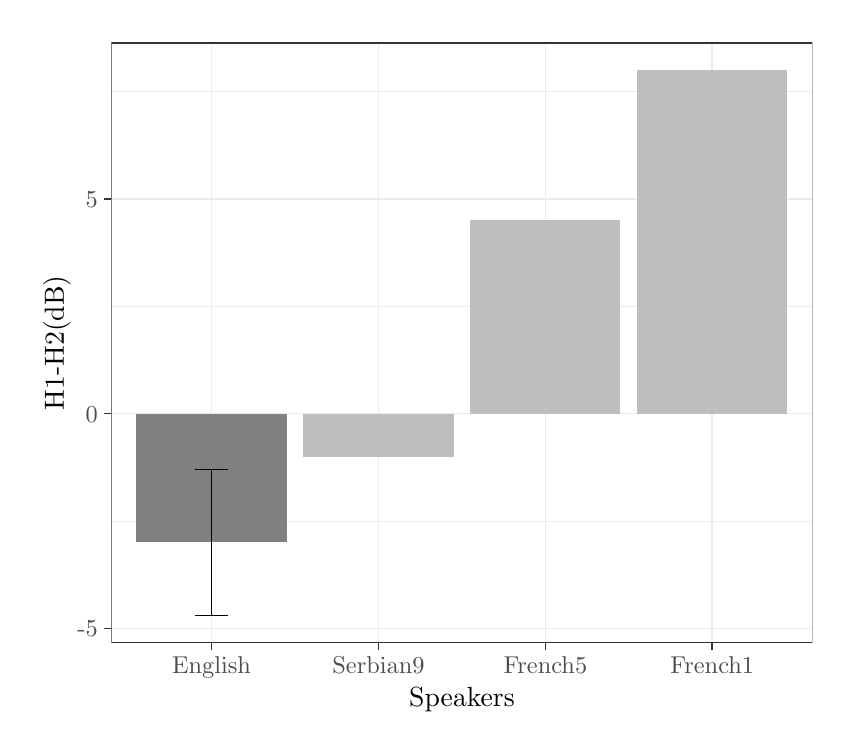
\begin{tikzpicture}[x=1pt,y=1pt]
\definecolor{fillColor}{RGB}{255,255,255}
\path[use as bounding box,fill=fillColor,fill opacity=0.00] (0,0) rectangle (289.08,252.94);
\begin{scope}
\path[clip] (  0.00,  0.00) rectangle (289.08,252.94);
\definecolor{drawColor}{RGB}{255,255,255}
\definecolor{fillColor}{RGB}{255,255,255}

\path[draw=drawColor,line width= 0.6pt,line join=round,line cap=round,fill=fillColor] (  0.00,  0.00) rectangle (289.08,252.94);
\end{scope}
\begin{scope}
\path[clip] ( 30.25, 30.69) rectangle (283.58,247.45);
\definecolor{fillColor}{RGB}{255,255,255}

\path[fill=fillColor] ( 30.25, 30.69) rectangle (283.58,247.45);
\definecolor{drawColor}{gray}{0.92}

\path[draw=drawColor,line width= 0.3pt,line join=round] ( 30.25, 74.67) --
	(283.58, 74.67);

\path[draw=drawColor,line width= 0.3pt,line join=round] ( 30.25,152.25) --
	(283.58,152.25);

\path[draw=drawColor,line width= 0.3pt,line join=round] ( 30.25,229.83) --
	(283.58,229.83);

\path[draw=drawColor,line width= 0.6pt,line join=round] ( 30.25, 35.88) --
	(283.58, 35.88);

\path[draw=drawColor,line width= 0.6pt,line join=round] ( 30.25,113.46) --
	(283.58,113.46);

\path[draw=drawColor,line width= 0.6pt,line join=round] ( 30.25,191.04) --
	(283.58,191.04);

\path[draw=drawColor,line width= 0.6pt,line join=round] ( 66.44, 30.69) --
	( 66.44,247.45);

\path[draw=drawColor,line width= 0.6pt,line join=round] (126.75, 30.69) --
	(126.75,247.45);

\path[draw=drawColor,line width= 0.6pt,line join=round] (187.07, 30.69) --
	(187.07,247.45);

\path[draw=drawColor,line width= 0.6pt,line join=round] (247.39, 30.69) --
	(247.39,247.45);
\definecolor{fillColor}{gray}{0.50}

\path[fill=fillColor] ( 39.29, 66.92) rectangle ( 93.58,113.46);
\definecolor{fillColor}{RGB}{190,190,190}

\path[fill=fillColor] ( 99.61, 97.95) rectangle (153.90,113.46);

\path[fill=fillColor] (159.93,113.46) rectangle (214.21,183.29);

\path[fill=fillColor] (220.25,113.46) rectangle (274.53,237.59);
\definecolor{drawColor}{RGB}{0,0,0}

\path[draw=drawColor,line width= 0.6pt,line join=round] ( 60.40, 93.29) --
	( 72.47, 93.29);

\path[draw=drawColor,line width= 0.6pt,line join=round] ( 66.44, 93.29) --
	( 66.44, 40.54);

\path[draw=drawColor,line width= 0.6pt,line join=round] ( 60.40, 40.54) --
	( 72.47, 40.54);

\definecolor{drawColor}{gray}{0.20}

\path[draw=drawColor,line width= 0.6pt,line join=round,line cap=round] ( 30.25, 30.69) rectangle (283.58,247.45);
\end{scope}
\begin{scope}
\path[clip] (  0.00,  0.00) rectangle (289.08,252.94);
\definecolor{drawColor}{gray}{0.30}

\node[text=drawColor,anchor=base east,inner sep=0pt, outer sep=0pt, scale=  0.88] at ( 25.30, 32.85) {-5};

\node[text=drawColor,anchor=base east,inner sep=0pt, outer sep=0pt, scale=  0.88] at ( 25.30,110.43) {0};

\node[text=drawColor,anchor=base east,inner sep=0pt, outer sep=0pt, scale=  0.88] at ( 25.30,188.01) {5};
\end{scope}
\begin{scope}
\path[clip] (  0.00,  0.00) rectangle (289.08,252.94);
\definecolor{drawColor}{gray}{0.20}

\path[draw=drawColor,line width= 0.6pt,line join=round] ( 27.50, 35.88) --
	( 30.25, 35.88);

\path[draw=drawColor,line width= 0.6pt,line join=round] ( 27.50,113.46) --
	( 30.25,113.46);

\path[draw=drawColor,line width= 0.6pt,line join=round] ( 27.50,191.04) --
	( 30.25,191.04);
\end{scope}
\begin{scope}
\path[clip] (  0.00,  0.00) rectangle (289.08,252.94);
\definecolor{drawColor}{gray}{0.20}

\path[draw=drawColor,line width= 0.6pt,line join=round] ( 66.44, 27.94) --
	( 66.44, 30.69);

\path[draw=drawColor,line width= 0.6pt,line join=round] (126.75, 27.94) --
	(126.75, 30.69);

\path[draw=drawColor,line width= 0.6pt,line join=round] (187.07, 27.94) --
	(187.07, 30.69);

\path[draw=drawColor,line width= 0.6pt,line join=round] (247.39, 27.94) --
	(247.39, 30.69);
\end{scope}
\begin{scope}
\path[clip] (  0.00,  0.00) rectangle (289.08,252.94);
\definecolor{drawColor}{gray}{0.30}

\node[text=drawColor,anchor=base,inner sep=0pt, outer sep=0pt, scale=  0.88] at ( 66.44, 19.68) {English};

\node[text=drawColor,anchor=base,inner sep=0pt, outer sep=0pt, scale=  0.88] at (126.75, 19.68) {Serbian9};

\node[text=drawColor,anchor=base,inner sep=0pt, outer sep=0pt, scale=  0.88] at (187.07, 19.68) {French5};

\node[text=drawColor,anchor=base,inner sep=0pt, outer sep=0pt, scale=  0.88] at (247.39, 19.68) {French1};
\end{scope}
\begin{scope}
\path[clip] (  0.00,  0.00) rectangle (289.08,252.94);
\definecolor{drawColor}{RGB}{0,0,0}

\node[text=drawColor,anchor=base,inner sep=0pt, outer sep=0pt, scale=  1.00] at (156.91,  7.64) {Speakers};
\end{scope}
\begin{scope}
\path[clip] (  0.00,  0.00) rectangle (289.08,252.94);
\definecolor{drawColor}{RGB}{0,0,0}

\node[text=drawColor,rotate= 90.00,anchor=base,inner sep=0pt, outer sep=0pt, scale=  1.00] at ( 13.08,139.07) {H1-H2(dB)};
\end{scope}
\end{tikzpicture}

  %\includegraphics[width=0.75\textwidth]{figures/phonation.png}
    \caption{Voice Quality Comparisons between L1 and L2 Productions of /ɪ/}
    \label{fig:h1h2}
  \figSpace
\end{figure}

Figure \ref{fig:h1h2} shows the average H1-H2 values of L1 and L2 segments. The three L2 speech samples involving the raising of [ɪ] in “\textit{six}” were all produced by females. Therefore, the comparison below illustrates only the difference between the three female L2 productions and all female L1 productions. As the figure shows, all three L2 speakers’ pronunciation had a relatively higher degree of breathiness (i.e., higher H1-H2 values) than the L1 speaker norm. The Serbian speaker’s production is less breathy than the other two L2 speakers; it is nevertheless breathier than the native mean. The fact that the SAA transcribers perceived high vowels with breathy quality as [i] is consistent with previous findings on the effect of voice quality on vowel height perception \citep{Lotto_1997}. The IPA transcriptions for these L2 speech samples were therefore accepted by the current study to represent vowel tensing. 



\subsection{Summary of Segmental Analysis}

The current study selected four types of L2 speech samples. Stimuli selection was based on IPA transcriptions available in the SAA. The most common L1 productions in the SAA were considered the L1 target productions. L2 speech samples that were transcribed the same as their L1 target productions were termed as the match stimuli. L2 speech samples whose IPA transcriptions differ from transcriptions of their L1 target productions were termed as the mismatch stimuli. The sections above described two types of mismatch stimuli. The first type consists of 25 L2 speech samples that were termed consonant mismatch. IPA transcriptions for these L2 speech samples differ from their L1 target productions by only one consonant. The second type consists of 25 L2 speech samples that were termed vowel mismatch. IPA transcriptions for these L2 speech samples differ from their L1 target productions by only one vowel. 

Acoustic analysis was conducted to examine the reliability of the IPA transcriptions. As shown in the analysis above, acoustic differences between the L2 speech samples and their corresponding L1 speech samples could be captured by IPA transcriptions of the L2 speech samples. The current study, therefore, considered these IPA transcriptions reliable. Audio files of these L2 speech samples were thus used by the current study as stimuli in two perception studies (Chapters 4 and 5). 

The third type of mismatch was termed syllable mismatch, because it concerns syllable structure differences between an L2 speech sample and its L1 target production. While consonant or vowel changes preserve the original syllable structure, segment deletion or segment epenthesis changes the original structure. The next section describes the selection of the 25 speech samples with syllable mismatches.

\subsection{Syllable Structures}

Structural variations investigated by the current study involve vowel epenthesis and consonant deletion. Co-articulatory properties and/or L1 phonotactics could, to some degree, generate a perceptual illusion of segment insertion, often termed as the “ghost segments” or “illusory segments” \citep{Dupoux_1999}. To select stimuli with potential structural problems, L2 audio samples were inspected in PRAAT to rule out possible cases of illusory perception. The following section uses two examples to illustrate how the inspections were carried out. As mentioned previously, the most common L1 productions in the SAA were considered representatives of L1 target productions. For example, the majority of the 100 surveyed L1 speakers of American English pronounced the word “\textit{ask}” in phrase “\textit{ask her}” as [æsk], while only one of the 100 L1 speakers pronounced the “\textit{ask}” as [æs]. [æsk] was therefore considered the L1 target production. [æs] was considered as a production with syllable mismatch. In other words, productions with mismatches are uncommon in L1 speech, but they are not necessarily unique to L2 speakers. 

To select L2 speech samples whose syllable structure differ from L1 target productions, the current study selected 25 L2 speech samples from the SAA based on their respective IPA transcriptions. To further inspect the reliability of the IPA transcriptions, acoustic information of the L2 speech samples were examined in PRAAT. If spectral information of a segment was missing from an L2 speech sample but existed in L1 target productions, then the L2 speech sample was considered as a stimulus with syllable mismatch. More specifically, it was considered a stimulus with segment deletion. Alternatively, if spectral information of a segment existed in an L2 speech sample but was missing from L1 target productions, then the L2 speech sample was considered as a stimulus with segment insertion.

\subsubsection{Segment Deletion}

Figure \ref{fig:del} shows the spectrogram of an L1 production and an L2 production of “\textit{ask her}”, where the dotted lines represent pitch contours and the solid lines represent intensity contours. The graph on the left illustrates an L1 production, which shows visible stop closure and burst after /s/. These characteristics are absent from the L2 production on the right, indicating that coda /k/ was dropped by the L2 speaker.

\begin{figure}[h!]
  \figSpace
    \centering
	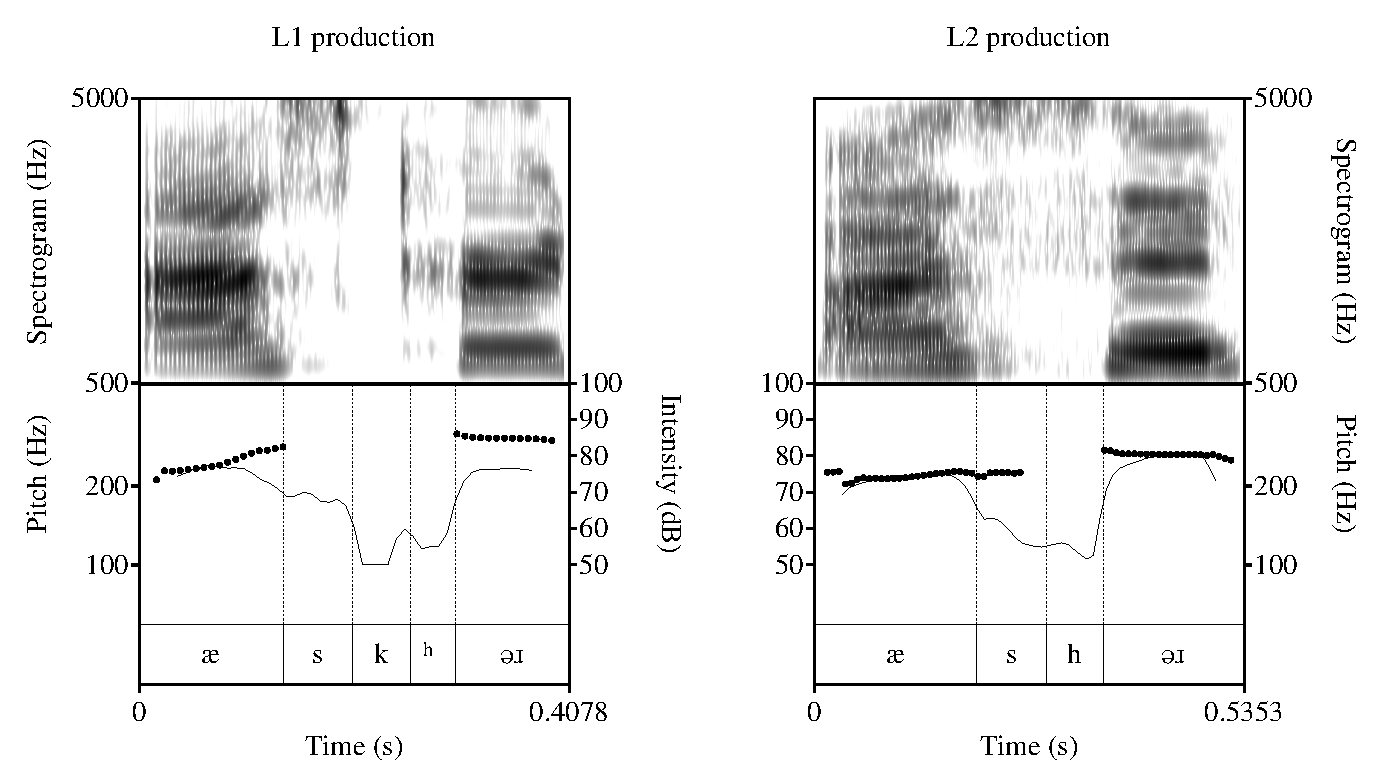
\includegraphics[width=1\textwidth]{figures/chp3/kdel.eps}
    \caption{/k/-Deletion in “\textit{ask her}”}
    \label{fig:del}
  \figSpace
\end{figure}

\subsubsection{Segment Insertion}

Eight stimuli were included in the current study to represent three types of segment insertions. Two stimuli involved prothesis of s-clusters (i.e., [sp]$\rightarrow$[əsp] in “\textit{six spoons}”); three stimuli involved anaptyxis of /pl/-clusters (i.e., /pl/ to /pəl/ in “\textit{please call}”); two stimuli represent paragoge at the end of “\textit{ask}” (i.e., [æsk]$\rightarrow$[æskə]), and one stimulus represents paragoge at the end of “five” (i.e. [faɪv] to [faɪvə]). The SAA transcribers marked discourse fillers and epenthetic vowels differently. A space was added between discourse fillers and their adjacent segments (e.g., [æsk ə həɹ]). No space was added between epenthetic vowels and the segment they epenthesize to (e.g., [æskə həɹ]). Speech samples with discourse fillers were not selected. The eight stimuli all contain epenthetic vowels as indicated by their respective IPA transcriptions. 

Figure \ref{fig:epen} illustrates a case of paragoge. The speech sample was produced by a Korean speaker who inserted a /ə/-like vocoid at the end of the word “\textit{ask}.” The epenthesized vocoid was transcribed by the SAA transcribers as a [ə]. 

\begin{figure}[h!]
  \figSpace
    \centering
	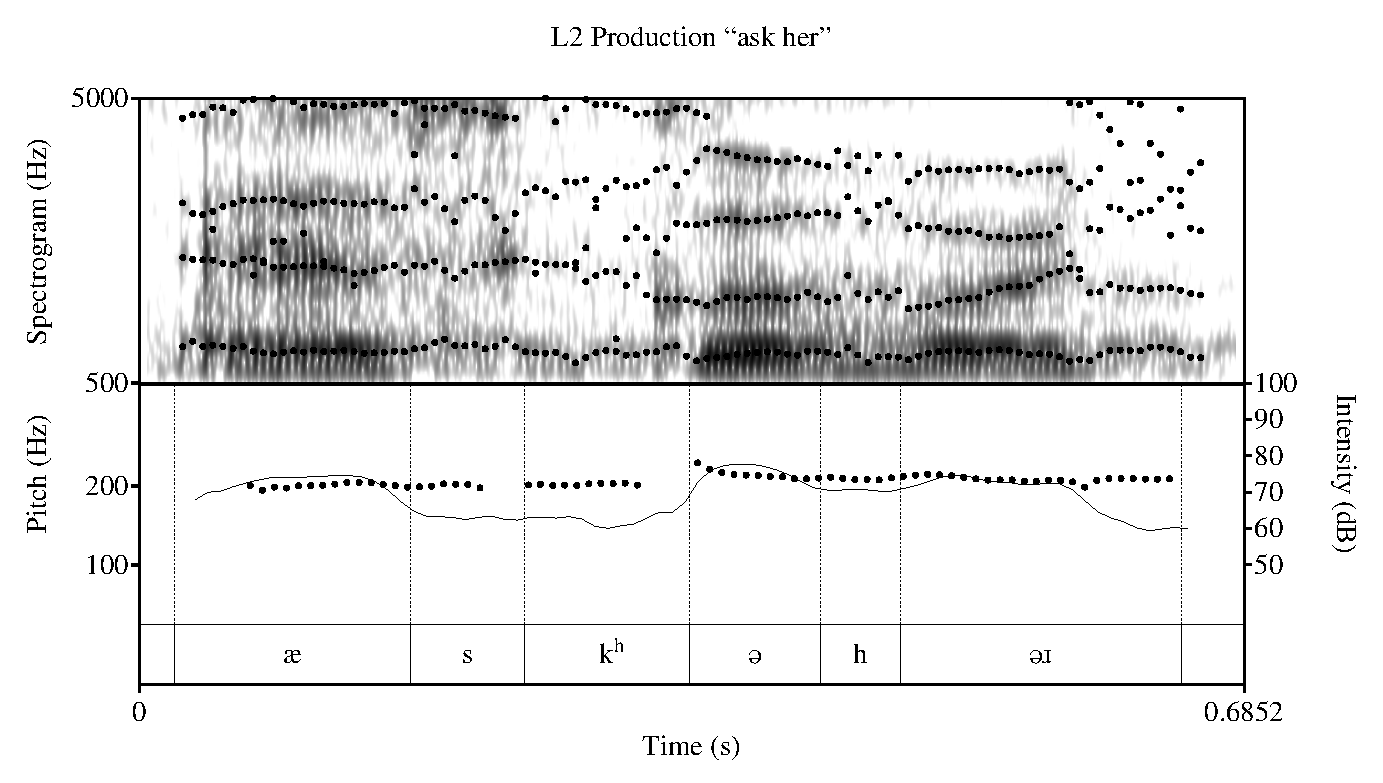
\includegraphics[width=0.8\textwidth]{figures/chp3/insert.eps}
    \caption{Paragoge after “\textit{ask}”}
    \label{fig:epen}
  \figSpace
\end{figure}

Spectral inspection carried out by the current study has successfully identified the epenthesized vocoid because it shows clear formant structures, carries pitch, and contains an intensity peak. These characteristics were utilized in the inspection of all other cases of segment insertion. Of the eight cases inspected, seven of them satisfy the aforementioned criteria. The prothetic vocoid of /sp/ does not carry pitch, yet it contains clear formant structures and an intensity peak. One could argue against defining such vocoid, and indeed all the other seven vocoids, as epenthetic vowels. As previous research often shows, epenthetic vowels, transitional vowels and extended sonorants are sometimes difficult to distinguish, and definitions of epenthetic vowels vary from language to language \citep{Gouskova_2009, Hall_2011, Hall_2003}. 

The current study took an impressionistic approach with regard to vowel epenthesis. As long as the epenthesized segment has clear formant structure and was transcribed with a [ə] or [ɪ], it is considered an epenthetic vocoid.  In summary, IPA transcriptions of the 25 L2 speech samples were verified via the process discussed above. The 25 L2 speech samples were selected as stimuli with syllable mismatches. 

\section{Summary}

The current study selected 100 L2 speech samples as stimuli in two perception studies. The L2 speech samples were chosen based primarily on their IPA transcriptions in the SAA. To observe the potential effects of phonological context on accentedness perception, five phonological contexts from the so-called “Stella” passage were chosen. Each context was represented by 20 L2 speech samples, yielding 100 L2 speech samples in total. To determine the L1 target productions for the five contexts, IPA transcriptions of 100 L1 speakers of American English from the SAA were surveyed to find the most common productions (e.g., [pʰliz kʰɑl] for “\textit{please call}”). L2 speech samples that were transcribed the same as their L1 target productions were termed as the match stimuli. L2 speech samples that were not transcribed as the same as their L1 target productions were termed as the mismatch stimuli. 

Among the 20 L2 speech samples for each of the five contexts, five speech samples were the match stimuli (e.g., [pʰliz kʰɑl] for “\textit{please call}”). The rest 15 L2 speech samples were the mismatch stimuli. Among the 15 mismatch stimuli, five differed from their L1 target production by only one consonant (e.g., [pʰlis kʰɑl] for “\textit{please call}”), five differed from their L1target production by only one vowel (e.g., [pʰliz kʰol] for “\textit{please call}”). Another five L2 speech samples, did not differ from their L1 target production segmentally, but contained either one more or one less segment than their L1 target productions (e.g., [pʰəliz kʰɑl] or [pʰliz kʰɑ] for “\textit{please call}”). These three types of stimuli were termed consonant mismatch, vowel mismatch, and syllable mismatch respectively. 

To verify the reliability of the IPA transcriptions for the 100 L2 stimuli, acoustic analysis was performed to compare L2 speech samples with their L1 counterparts. Speech samples from 50 L1 speakers of American English were extracted from the SAA for the analysis of native speaker pronunciation norms, which were approximated by the mean L1 values of relevant benchmark acoustic measurements (e.g., mean L1 VOT duration, mean L1 COG, mean L1 F1/F2/F3 values etc.). Results showed that acoustic differences between the L2 stimuli and native speaker norms were successfully captured by the IPA transcriptions. The current study therefore concluded that these IPA transcriptions for the 100 L2 stimuli are reliable. These stimuli were then used in two perception studies to elicit accentedness judgment from L1 listeners of American English. 
































